\documentclass[12pt, twoside, a4paper, openright]{report}

%packages-----------------------------------------------------------------------

\usepackage[utf8]{inputenc}
\usepackage[english]{babel}
\usepackage[T1]{fontenc}
\usepackage{lmodern}
\usepackage{array}
%\usepackage{times}
%\usepackage{charter}
\usepackage{graphicx}
\usepackage{color}
\usepackage{amsmath}
\usepackage{amssymb}
\usepackage{amsthm}
\usepackage{verbatim}
\usepackage{pdfpages}
\usepackage[unicode]{hyperref}
\usepackage[small, bf]{caption}
\usepackage{enumerate}
\usepackage{epstopdf}
\usepackage{epsfig}
\usepackage{setspace}
\usepackage{esdiff}
\usepackage{enumitem}
\usepackage[inner=2.5cm, outer=2cm]{geometry}
\usepackage{emptypage}
\usepackage{caption}
%\usepackage{subcaption}
\usepackage{listings}
\usepackage{color}
\usepackage{multicol}
\usepackage{lipsum}
\usepackage{mathabx}
\usepackage{floatrow}
\usepackage{courier}
\usepackage[position=top]{subfig}

%fancystyles--------------------------------------------------------------------

\usepackage{fancyhdr}

\fancypagestyle{myfancy}{

\fancyhead[LE]{\nouppercase{\leftmark}}
\fancyhead[LO]{}
\fancyhead[CO]{}
\fancyhead[CE]{}
\fancyhead[RE]{}
\fancyhead[RO]{\nouppercase{\rightmark}}

\fancyfoot[LE]{\thepage}
\fancyfoot[LO]{}
\fancyfoot[CO]{}
\fancyfoot[CE]{}
\fancyfoot[RE]{}
\fancyfoot[RO]{\thepage}

\renewcommand{\headrulewidth}{0.4pt}
\renewcommand{\footrulewidth}{0.0pt}
}

\fancypagestyle{plain}{

\fancyhead[LE]{}
\fancyhead[LO]{}
\fancyhead[CO]{}
\fancyhead[CE]{}
\fancyhead[RE]{}
\fancyhead[RO]{}

\fancyfoot[LE]{\thepage}
\fancyfoot[LO]{}
\fancyfoot[CO]{}
\fancyfoot[CE]{}
\fancyfoot[RE]{}
\fancyfoot[RO]{\thepage}

\renewcommand{\headrulewidth}{0.0pt}
\renewcommand{\footrulewidth}{0.0pt}
}

%tikz---------------------------------------------------------------------------

\usepackage{tikz}
\usetikzlibrary{shapes, arrows}

%url----------------------------------------------------------------------------

\usepackage{url}
\DeclareUrlCommand\url{\def\UrlLeft{<}\def\UrlRight{>} \urlstyle{tt}}

%color--------------------------------------------------------------------------

\definecolor{darkred}{rgb}{0.6,0,0}
\definecolor{darkgreen}{rgb}{0,0.6,0}
\definecolor{darkblue}{rgb}{0,0,0.6}
\definecolor{darkgrey}{rgb}{0.3,0.3,0.3}
\definecolor{grey}{rgb}{0.6,0.6,0.6}
\definecolor{lightgrey}{rgb}{0.95,0.95,0.95}
\definecolor{lightred}{rgb}{0.99,0.85,0.85}
\definecolor{violet}{rgb}{0.65,0.45,0.75}

%listings-----------------------------------------------------------------------

\definecolor{mygreen}{rgb}{0,0.6,0}
\definecolor{mygray}{rgb}{0.5,0.5,0.5}
\definecolor{light}{rgb}{0.96, 0.96, 0.96}
\definecolor{mymauve}{rgb}{0.58,0,0.82}

\lstdefinestyle{CXX} {
	language=C++,
	backgroundcolor=\color{light},
	basicstyle=\scriptsize\ttfamily,
	breakatwhitespace=false,
	breaklines=true,
	captionpos=t,
	commentstyle=\color{mygreen},
	deletekeywords={},
	escapeinside={\%*}{*)},
	extendedchars=true,
	frame=single,
	keepspaces=true,
	keywordstyle=\color{blue},
	otherkeywords={},
	numbers=left,
	numbersep=5pt,
	numberstyle=\tiny\color{mygray},
	rulecolor=\color{black},
	showspaces=false,
	showstringspaces=false, 
	showtabs=false,
	stepnumber=1,
	stringstyle=\color{mymauve},
	tabsize=3,
	title=\lstname   
}

\lstdefinestyle{FORTRAN} {
	language=[90]Fortran,
	backgroundcolor=\color{light},
	basicstyle=\scriptsize\ttfamily,
	keywordstyle=\color{blue},
	commentstyle=\color{mygreen},
	breakatwhitespace=false,
	breaklines=true,
	captionpos=t,
	deletekeywords={},
	escapeinside={\%*}{*)},
	extendedchars=true,
	frame=single,
	keepspaces=true,
	otherkeywords={},
	numbers=left,
	numbersep=5pt,
	numberstyle=\tiny\color{mygray},
	rulecolor=\color{black},
	showspaces=false,
	showstringspaces=false, 
	showtabs=false,
	stepnumber=1,
	stringstyle=\color{mymauve},
	tabsize=3,
	title=\lstname 
}

%settings-----------------------------------------------------------------------

\setlength{\parindent}{20pt}
\setlength{\parskip}{0pt plus 0.05pt minus 0.05pt}
\pagenumbering{arabic}
\frenchspacing

\DeclareFontFamily{U}{mathx}{\hyphenchar\font45}
\DeclareFontShape{U}{mathx}{m}{n}{<-> mathx10}{}
\DeclareSymbolFont{mathx}{U}{mathx}{m}{n}
\DeclareMathAccent{\widebar}{0}{mathx}{"73}

%commands-----------------------------------------------------------------------

\renewcommand{\baselinestretch}{1.0}

\newcommand{\ctu}{Czech Technical University in Prague }
\newcommand{\fnspe}{Faculty of Nuclear Sciences and Physical Engineering }
\newcommand{\dpe}{Department of Physical Electronics }
\newcommand{\branch}{Computational Physics }

\newcommand{\projecttitle}{Tight-focusing of short intense laser pulses in~PIC~simulations of laser-plasma~interaction }
\newcommand{\projecttitlecz}{Zaostření krátkého intenzivního laserového impulsu do velmi malého ohniska v PIC simulacích interakce s plazmatem }

\newcommand{\valenta}{Bc. Petr Valenta }
\newcommand{\klimo}{doc. Ing. Ondřej Klimo, Ph.D. }
\newcommand{\weber}{Dr. Stefan Andreas Weber }
\newcommand{\academicyear}{2016/2017 }

\newcommand{\keywords}{}
\newcommand{\projectabstract}{}

%macros-------------------------------------------------------------------------

\newcommand{\nucl}[3]{
\ensuremath{
\phantom{
\ensuremath{^{#1}_{#2}}}
\llap{\ensuremath{^{\rule{0pt}{0pt}#1}}}
\llap{\ensuremath{_{\rule{0pt}{7pt}#2}}}
\mbox{#3}}}

\newcommand{\norm}[1]{\lVert#1\rVert}
\newcommand{\abs}[1]{\lvert#1\rvert}

\renewcommand{\vec}[1]{\mathbf{#1}}

\newcommand{\rot}[1]{\nabla \times #1}
\newcommand{\grad}[1]{\nabla #1}
\renewcommand{\div}[1]{\nabla \cdot #1}
\newcommand{\laplace}[1]{\Delta #1}
\newcommand{\dalembert}[1]{\Box #1}

\newcommand{\e}[0]{\mathrm{e}}
\renewcommand{\i}[0]{\mathrm{i}}
\renewcommand{\d}[0]{\mathrm{d}}

%changecountering---------------------------------------------------------------

\usepackage{chngcntr}
%\counterwithout{equation}{chapter}
\counterwithout{figure}{chapter}
\counterwithout{table}{chapter}

%document-----------------------------------------------------------------------

\begin{document}

\pagestyle{empty}

%1------------------------------------------------------------------------------

%\mbox{}
%\newpage

\begin{titlepage}

\begin{center}
{\Large \bf \ctu}\\[4mm]
{\Large \bf \fnspe}\\[4mm]
{\Large \bf \dpe}\\[16mm]
\epsfysize=45mm \epsffile{img/logo/ctu.eps}\\[12mm]
\begin{spacing}{2.0}
{\LARGE \bf \projecttitle}\\[2mm]
\end{spacing}
{\Large (Master thesis)} \\
\vfill
\end{center}

\begin{flushleft}
\begin{tabular}{rl}
Author: & \valenta \\[1mm]
Supervisor: & \klimo \\[1mm]
Consultant: & \weber \\[1mm]
Academic year: & \academicyear \\[1mm]
\end{tabular}
\end{flushleft}

\end{titlepage}

%2------------------------------------------------------------------------------

\newpage
\mbox{}

%3------------------------------------------------------------------------------

\newpage
\includepdf[pages=1]{dat/zadani.pdf}

%4------------------------------------------------------------------------------

\newpage
\includepdf[pages=2]{dat/zadani.pdf}

%5------------------------------------------------------------------------------

\newpage
\null
\vfill
{\bf \noindent Prohlášení/Declaration} \\[5mm]
Prohlašuji, že jsem předloženou práci vypracoval samostatně a že jsem uvedl veškerou
použitou literaturu.\\[2mm]
I declare that I carried out this work independently, and only with the cited sources, literature and other professional sources.\\
\vspace{5mm}V Praze dne/In Prague on .............................\hfill
\begin{tabular}{c}
........................................\\
\valenta
\end{tabular}

%6------------------------------------------------------------------------------

\newpage
\thispagestyle{empty}
\mbox{}

%7------------------------------------------------------------------------------

\newpage
\begin{flushleft}
	\renewcommand{\arraystretch}{1.3}
	\begin{tabular}{r p{12cm}}
		Název práce:
		~ & \bf \projecttitlecz \\
		Autor:
		~ & \valenta \\
		Druh práce:
		~ & Diplomová práce \\
		Studijní program:
		~ & (N3913) Aplikace přírodních věd\\
		Vedoucí práce:
		Obor:
		~ & (3901T065) Informatická fyzika\\
		Vedoucí práce:
		~ & \klimo \newline Katedra fyzikální elektroniky, Fakulta jaderná a fyzikálně inženýrská, České vysoké učení technické v Praze \\
		Konzultant:
		~ & \weber \newline Projekt ELI-Beamlines, Fyzikální ústav Akademie věd České republiky, v. v. i. \\
	\end{tabular}
\end{flushleft}

\begin{center}
\textbf{Abstrakt}\\
\end{center}

Content...\\

Klíčová slova:


%8------------------------------------------------------------------------------

\newpage
\begin{flushleft}
	\renewcommand{\arraystretch}{1.3}
	\begin{tabular}{r p{12cm}}
		Title:
		~ & \bf \projecttitle \\
		Author:
		~ & \valenta \\
		Type of work:
		~ & Master thesis \\
		Study programme:
		~ & (N3913) Aplications of Natural Sciences	 \\
		Branch of study:
		~ & (3901T065) Computational Physics \\
		Supervisor:
		~ & \klimo \newline Department of Physical Electronics, Faculty of Nuclear Sciences and Physical Engineering, Czech Technical University in Prague \\
		Consultant:
		~ & \weber \newline Project ELI-Beamlines, Institute of Physics, The Czech Academy of Sciences, v. v. i. \\
	\end{tabular}
\end{flushleft}

\begin{center}
	\textbf{Abstract}\\
\end{center}

Content...\\

Keywords: plasma-based amplification, PIC simulations, parametric instabilities

%9------------------------------------------------------------------------------

\tableofcontents
\addtocontents{toc}{\protect\thispagestyle{empty}}
\thispagestyle{empty}

%-------------------------------------------------------------------------------

\pagestyle{myfancy}

\chapter*{Introduction\markboth{Introduction}{Introduction}}
\addcontentsline{toc}{chapter}{Introduction}
Since the first demonstration of pulsed laser in 1960 \cite{Maiman1960}, the intensive research and development in the field of laser technology have seen a tremendous progress. Pulse compression and amplification techniques, such as CPA \cite{StricklandMourou1985}, OPCPA \cite{Dubietis1992} and lately RBA \cite{Malkin1999}, have enabled a generation of ultra-short laser pulses with intensities exceeding $ 10^{22} \ \mathrm{W/cm^{2}} $. Pulses in this regime provide an unprecedented capability for basic research (e.g. high-energy density physics, warm dense matter, plasma optics, laboratory astrophysics) as well as a broad range of groundbreaking applications in diverse fields (e.g. coherent diffractive imaging, X-ray diffraction and spectroscopy, production of compact sources for radiotherapy, inertial confinement fusion).

The peak laser intensities are typically increased by enhancing the produced laser properties, either by lowering the pulse duration or increasing the pulse energy. This approach comes at great cost since it requires a higher level of complexity for the laser chain \cite{Fuchs2014}. More effective way to increase the laser intensity is to reduce the focal spot size. However, the conventional solid state optics are inappropriate in the case of tight-focusing (expensive, susceptible to damage from solid target debris, sensitive to small misalignments). Nevertheless, it seems that many drawbacks might be in future overcome by using a plasma-based focusing optics. Therefore, the interaction of tightly focused laser beams with matter is currently attracting much attention \cite{Popov2008, Popov2009, Lifschitz2016, Yan2005}. 

This work is structured as follows: the first chapter provides a brief introduction to the classical electromagnetic field theory, including the mathematical derivation of the paraxial Gaussian beam formula. The second chapter summarizes the elementary knowledge of plasma physics and physics of laser-plasma interaction. In the third chapter, one of the most popular numerical methods in plasma physics, particle-in-cell (PIC), is thoroughly discussed. The characteristics and features of the code EPOCH \cite{bennett}, which has been used for the simulations within this work, can be found in the last section of this chapter. The fourth chapter is devoted to the tight-focusing of laser pulses, including a description of algorithm for rigorous calculation of electromagnetic fields at boundaries of simulation domain \cite{Thiele2016}. This chapter also contains the details about the implementation of the algorithm as well as thorough evaluation of its correctness and the correctness of the implementation. At the end, one may find the overview of currently used experimental methods for tight-focusing. The last chapter demonstrates the results of several large-scale two-dimensional simulations employing tightly focused laser beams interacting with solid targets.

Although the most convenient unit system for most plasma applications is the Gaussian cgs system, throughout this work the SI (System Internationale) units are used, unless explicitly stated. Symbols in bold represent vector quantities, and symbols in italics represent scalar quantities, unless otherwise indicated.


%-------------------------------------------------------------------------------

\chapter{Electromagnetic field}
Since the laser beam is nothing but the electromagnetic wave, the opening chapter has to be logically devoted to the principles of the classical electromagnetic field theory based on the elegant Maxwell's equations. The reader can find brief description of the microscopic as well as macroscopic variant of the Maxwell's equations with corresponding constitutive relations and their general solutions exploiting electrodynamic potentials and Hertz vectors. A short part is devoted also to energy and momentum of the electromagnetic waves. In the last part, one can find the simplest mathematical description of the focused laser beam.

\section{Maxwell's equations}
In order to achieve fusion, the reacting nuclei have to get very close to each other to activate the strong nuclear force. However, there is a large electrostatic repulsion between them as they come together because the protons in nuclei are positively charged. There are several possibilities of overcoming this barrier. One can for example utilize the initial kinetic energy of the chaotic thermal motion of the particles. In thermal equilibrium, the Coulomb collisions redistribute the kinetic energy among the plasma particles, and fusion reactions will eventually occur after a sequence of collisions. This approach is called thermonuclear fusion.

Reactions which could be usable in the case of the energy production on Earth must have high cross-section values at relatively low required incident energies. Furthermore, the economic viability and competitiveness is crucial for commercial use of fusion power. In other words, the reaction must be able to cover obviously no less than the energetic costs incurred for its ignition. The word ignition refers to the moment when a controlled fusion reaction generates as much or more energy than is needed to spark the reaction. In regards to each of these attributes, the best reaction candidate appears to be the reaction of two hydrogen isotopes - deuterium and tritium,
\begin{equation}
\nucl{2}{1}{H} + \nucl{3}{1}{H} \rightarrow \nucl{4}{2}{He} \ \mathrm{(3{,}5 \ MeV)} + \nucl{1}{0}{n} \ \mathrm{(14{,}1 \ MeV)}.
\end{equation}

Deuterium has quite rich natural abundance in Earth's oceans, thus it is commonly available in sufficient quantity. The efficient extraction from seawater is supposed to be technically ready \cite{bradshaw}. On the contrary, naturally occurring tritium is extremely rare due to its short half-life, therefore the fuel cycle requires the breeding of tritium. The production is possible with irradiation of lithium by fusion neutrons using the following reaction,
\begin{equation}
\nucl{6}{3}{Li} + \nucl{1}{0}{n} \rightarrow \nucl{4}{2}{He} \ \mathrm{(2{,}1 \ MeV)} + \nucl{3}{1}{H} \ \mathrm{(2{,}7 \ MeV)}.
\end{equation}

Lithium is widely distributed in the Earth's crust and seawater. Consequently, both fusion fuel resources are relatively easily accessible, uniformly geographically distributed and have near unlimited availability. The product of their reaction is a neutron and a helium nucleus, of which the latter product is not radioactive. These attributes and the potential to produce large amounts of carbon-free energy with almost no environmental impact predetermine nuclear fusion to become a global energy source.

\section{Electrodynamic potentials}
The first-order partial differential Maxwell's equations can be effectively converted to a smaller number of second-order equations by introducing electrodynamic potentials. Hence, one can express the electric and magnetic field as follows \cite{Thide2011},
\begin{equation}
\label{1.12}
\vec{E} = -\grad{\Phi} - \diffp{\vec{A}}{t},
\end{equation}
\begin{equation}
\label{1.13}
\vec{B} = \rot{\vec{A}},
\end{equation}
where $ \Phi\left(\vec{r}, t \right) $ is the scalar potential and $ \vec{A}\left(\vec{r}, t \right) $ is the vector potential of the corresponding fields. One can clearly see that using the definitions \ref{1.12}, \ref{1.13}, six vector components are replaced by only four potential functions and two Maxwell's homogeneous equations (\ref{1.8}, \ref{1.9}) are fulfilled identically. 

However, by definitions \ref{1.12}, \ref{1.13}, $ \Phi\left(\vec{r}, t \right) $ and $ \vec{A}\left(\vec{r}, t \right) $ are not defined uniquely, thus an infinite number of potentials which lead to the same fields may be constructed. To avoid that, one has to impose a supplementary condition, for example
\begin{equation}
\label{1.14}
\div{\vec{A}} + \mu \varepsilon \diffp{\Phi}{t} = 0.
\end{equation}
The condition \ref{1.14} is called the Lorenz gauge \cite{Thide2011}. Lorenz gauge is commonly used in electromagnetism because of its independence of the coordinate system. Furthermore, it leads to the following uncoupled equations,
\begin{equation}
\label{1.15}
\laplace{\Phi} - \mu \varepsilon \diffp[2]{\Phi}{t} = -\frac{\rho}{\varepsilon},
\end{equation}
\begin{equation}
\label{1.16}
\laplace{\vec{A}} - \mu \varepsilon \diffp[2]{\vec{A}}{t} = -\mu \vec{J},
\end{equation}
that are in all respects equivalent to the Maxwell's equations and in many situations much simpler to solve.

Equations \ref{1.15}, \ref{1.16} correspond to the inhomogeneous wave equations for scalar potential $ \Phi\left(\vec{r}, t \right) $ and vector potential $ \vec{A}\left(\vec{r}, t \right) $. Their general solutions are given by the following expressions \cite{Thide2011},
\begin{equation}
\label{1.17}
\Phi\left(\vec{r}, t \right) = \frac{1}{4 \pi \varepsilon} \int \frac{\rho\left(\vec{r^{\: \prime}}, t^{\: \prime} \right)}{\norm{\vec{r} - \vec{r^{\: \prime}}}} \mathrm{d} V,
\end{equation}
\begin{equation}
\label{1.18}
\vec{A}\left(\vec{r}, t \right) = \frac{\mu}{4 \pi} \int \frac{\vec{J}\left(\vec{r^{\: \prime}}, t^{\: \prime} \right)}{\norm{\vec{r} - \vec{r^{\: \prime}}}} \mathrm{d} V,
\end{equation}
where $ \mathrm{d} V $ is a volume element and $ \norm{.} $ stands for the standard Euclidean norm. Note that the solutions \ref{1.17}, \ref{1.18} are dependent only on charge and current densities at position $ \vec{r^{\: \prime}} $ at so-called retarded time $ t^{\: \prime} = t - \sqrt{\mu \epsilon} \norm{\vec{r} - \vec{r^{\: \prime}}} $ which takes into account the finite velocity of the wave \cite{Feynman1963}. In other words, the fields at the observation point $ \vec{r} $ at the time $ t $ are proportional to the sum of all the electromagnetic waves that leave the source elements at point $ \vec{r^{\: \prime}} $ at the retarded time $ t^{\: \prime} $.

\section{Hertz vectors}
There exists also other possibilities how to express the electromagnetic field. Under ordinary conditions, an arbitrary electromagnetic field may be defined in terms of a single vector function \cite{Essex1977}. This may be helpful for solving of many problems of classical electromagnetic theory, particularly the wave propagation.

First, let us introduce the electric Hertz vector $ {\vec{\Pi_e}}\left(\vec{r}, t \right) $ in terms of the scalar and vector potentials \cite{Stratton2007},
\begin{equation}
\label{1.19}
\Phi = - \div{\vec{\Pi_e}},
\end{equation}
\begin{equation}
\label{1.20}
\vec{A} = \mu \varepsilon \diffp{\vec{\Pi_e}}{t}.
\end{equation}

Note that the definitions \ref{1.19}, \ref{1.20} are consistent with the Lorenz gauge condition \ref{1.14}. In the absence of magnetization, it might be easily shown that $ \vec{J} = \partial{\vec{P}}/\partial{t} $ and the electric Hertz vector $ {\vec{\Pi_e}}\left(\vec{r}, t \right) $ is governed by an inhomogeneous wave equation
\begin{equation}
\label{1.21}
\laplace{\vec{\Pi_e}} - \mu \varepsilon \diffp[2]{\vec{\Pi_e}}{t} = -\frac{\vec{P}}{\varepsilon}.
\end{equation}

The equation \ref{1.21} is of the same type as the equations \ref{1.15}, \ref{1.16} and has therefore the familiar general solution 
\begin{equation}
\label{1.22}
\vec{\Pi_e}\left(\vec{r}, t \right) = \frac{1}{4 \pi \varepsilon} \int \frac{\vec{P}\left(\vec{r^{\: \prime}}, t^{\: \prime} \right)}{\norm{\vec{r} - \vec{r^{\: \prime}}}} \mathrm{d} V.
\end{equation}

As might be seen form \ref{1.22}, the fields derived from the electric Hertz vector $ {\vec{\Pi_e}}\left(\vec{r}, t \right) $ can be interpreted as being due to a density distribution of electric dipoles \cite{Essex1977}. Every solution of \ref{1.22} then uniquely determines the electromagnetic field through
\begin{equation}
\label{1.23}
\vec{E} = \grad{\left(\div{\vec{\Pi_e}}\right)} - \mu \epsilon \diffp[2]{\vec{\Pi_e}}{t},
\end{equation}
\begin{equation}
\label{1.24}
\vec{B} = \mu \varepsilon \left(\rot{\diffp{\vec{\Pi_e}}{t}}\right).
\end{equation}

Second, one may introduce the magnetic Hertz vector $ {\vec{\Pi_m}}\left(\vec{r}, t \right) $ in terms of the scalar and vector potentials by the following expressions \cite{Stratton2007},
\begin{equation}
\label{1.25}
\Phi = 0,
\end{equation}
\begin{equation}
\label{1.26}
\vec{A} = \rot{\vec{\Pi_m}}.
\end{equation}
In the absence of polarization, $ \vec{J} = \rot{\vec{M}} $ and the magnetic Hertz vector $ {\vec{\Pi_m}}\left(\vec{r}, t \right) $ defined by \ref{1.25} and \ref{1.26} fulfills an inhomogeneous wave equation
\begin{equation}
\label{1.27}
\laplace{\vec{\Pi_m}} - \mu \varepsilon \diffp[2]{\vec{\Pi_m}}{t} = -\mu \vec{M}.
\end{equation}
As for the previous cases, one may easily find the solution of \ref{1.27},
\begin{equation}
\label{1.28}
\vec{\Pi_m}\left(\vec{r}, t \right) = \frac{\mu}{4 \pi} \int \frac{\vec{M}\left(\vec{r^{\: \prime}}, t^{\: \prime} \right)}{\norm{\vec{r} - \vec{r^{\: \prime}}}} \mathrm{d} V,
\end{equation}
thus the fields derived from the magnetic Hertz vector $ {\vec{\Pi_m}}\left(\vec{r}, t \right) $ may be imagined to be due to a density distribution of magnetic dipoles \cite{Essex1977}. Again, every solution of \ref{1.28} uniquely determines the electromagnetic field via
\begin{equation}
\label{1.29}
\vec{E} = \rot{\diffp{\vec{\Pi_m}}{t}},
\end{equation}
\begin{equation}
\label{1.30}
\vec{B} = \rot{\left(\rot{\vec{\Pi_m}}\right)}.
\end{equation}

Note that the above derivations considered electric and magnetic Hertz vectors as a separate quantities. It is also possible, however, to introduce them together in the form of one six-vector \cite{Nisbet1955}.

\section{Energy and momentum}
To be able to describe the interaction of electromagnetic field with matter, one has to know the energy distribution throughout the field as well as the momentum balance.

By scalar multiplications of \ref{1.9} by $ \vec{H}\left( \vec{r}, t \right) $, of \ref{1.10} by $ \vec{E}\left( \vec{r}, t \right) $, following subtraction of both obtained equations and using standard vector identities, one gets the expression 
\begin{equation}
\label{1.31}
\vec{E} \cdot \diffp{\vec{D}}{t} + \vec{H} \cdot \diffp{\vec{B}}{t} + \div{\left(\vec{E} \times \vec{H} \right)} = -\vec{E} \cdot \vec{J}.
\end{equation}
The equation \ref{1.31} can be rewritten in the form of conservation law,
\begin{equation}
\label{1.32}
\diffp{u}{t} + \div{\vec{S}} = - \vec{E} \cdot \vec{J},
\end{equation}
where
\begin{equation}
\label{1.33}
u = \frac{1}{2} \left(\vec{E} \cdot \vec{D} + \vec{H} \cdot \vec{B} \right), \quad \vec{S} = \vec{E} \times \vec{H}.
\end{equation}
The quantity $ u\left( \vec{r}, t \right) $ in \ref{1.33} describes the total energy density in the field and $ \vec{S}\left( \vec{r}, t \right) $ is so-called Poynting vector which represents the energy flow of the field.

The important statement \ref{1.32}, also referred to as the Poynting theorem, expresses the conservation of energy for the electromagnetic field. In other words, the time rate of change of the field energy within a certain region and the energy flowing out of that region is balanced by the conversion of the electromagnetic energy into mechanical or heat energy and vice-versa.

+momentum...

\noindent
Lorentz force:
\begin{equation}
\vec{F} = q \left(E + v \times B \right) 
\end{equation}
Ohm's law:
\begin{equation}
\vec{J} = \sigma \vec{E}
\end{equation}

\section{Electromagnetic waves and Gaussian beam}
In this section, the simplest mathematical description of a focused laser beam based on approximations to the wave equation is deduced. Since in numerical codes it is a common practice to prescribe the laser beams by their propagation in free space, the set of the microscopic Maxwell's equations \ref{1.1} - \ref{1.4} will be exploited.

In the absence of external sources, it might be easily shown that the equations \ref{1.1} - \ref{1.4} may be alternatively formulated as an uncoupled homogeneous wave equations for electric field $ \vec{E}\left( \vec{r}, t \right) $ and magnetic field $ \vec{B}\left( \vec{r}, t \right) $ \cite{Feynman1963},
\begin{equation}
\label{1.34}
\laplace{\vec{E}} - \frac{1}{c^{2}} \diffp[2]{\vec{E}}{t} = 0,
\end{equation}
\begin{equation}
\label{1.35}
\laplace{\vec{B}} - \frac{1}{c^{2}} \diffp[2]{\vec{B}}{t} = 0,
\end{equation}
where the universal constant $ c = 1/\sqrt{\mu_0 \varepsilon_0} $ is the speed of light in vacuum, which leads to the essential fact, that the electromagnetic waves propagate in vacuum with the velocity of light $ c $. However, the wave equations \ref{1.34}, \ref{1.35} do not provide all the information about the electric and magnetic field of the wave. There are further constraints due to Maxwell's equations restricting the orientation and proportional magnitudes of the fields. From the set \ref{1.1} - \ref{1.4}, it might be clearly seen that $ \vec{E}\left( \vec{r}, t \right) $ and $ \vec{B}\left( \vec{r}, t \right) $ must be mutually perpendicular to each other as well as to the direction of the wave propagation \cite{Stratton2007}. 

Without any loss of generality, consider the laser beam as a monochromatic electromagnetic wave propagating toward the positive direction of the z-axis. In many standard references, the description of such a wave is given by the evolution of a single electric field component linearly polarized along the x-axis of the Cartesian coordinate system \cite{Siegman1986, Milonni1988, Yariv1989, Svelto2010, Galvez2006} (although the more proper way would be to use the vector potential \cite{Davis1979, Davis1981, Guenther1990, Salamin2006, Vaveliuk2007}), therefore one has to look for the solution of the equation \ref{1.34}. 

According to the previous assumptions, the solution is expected to be in the form of the following plane wave,
\begin{equation}
\label{1.36}
\vec{E}\left(\vec{r_\bot}, z, t \right)  = \Re \ E_0 \Psi \left(\vec{r_\bot}, z \right) \e^{\i \left(k_z z - \omega t \right)} \mathrm{\vec{\hat{e}_x}},
\end{equation}
where $ \vec{r_\bot} = (x, y)^{\mathrm{T}} $ is the vector of transverse Cartesian coordinates, symbol $ \Re $ stands for the real part of the complex quantity, $ E_0 $ is a constant amplitude, $ \Psi \left(\vec{r_\bot}, z \right) $ is the part of the wave function which is dependent only on the spatial coordinates, $ \omega $ denotes the angular frequency, $ k_z $ is the z-component of the wave vector $ \vec{k}\left(\omega \right) $, $ \mathrm{i} $ denotes the imaginary unit and $ \mathrm{\vec{\hat{e}_x}} $ is the unit vector pointing in the direction of the x-axis.

Direct substitution of expression \ref{1.36} into the equation \ref{1.34} yields the time-independent form of the scalar wave equation
\begin{equation}
\label{1.37}
\laplace{\Psi \left(\vec{r_\bot}, z \right)} + 2 \i k_z \diffp{\Psi \left(\vec{r_\bot}, z \right)}{z} = 0.
\end{equation}
The equation \ref{1.37} is called the Helmholtz equation \cite{Born2013}. Note that it is sufficient to seek solutions to the equation \ref{1.37} since the wave \ref{1.36} is monochromatic.

It turned out, that the geometry of the focused laser beam can be expressed in terms of the laser wavelength $ \lambda $ and the following three parameters,
\begin{equation}
\label{1.38}
w_0, \qquad z_{\mathrm{R}} = \frac{k_z w_0^2}{2} = \frac{\pi w_0^2}{\lambda}, \qquad \Theta = \frac{w_0}{z_\mathrm{R}} = \frac{\lambda}{\pi w_0}.
\end{equation}
The parameter $ w_0 $ in \ref{1.38} is the beam waist, defined as a radius at which the laser intensity fall to $ 1/\e^2 $ of its axial value at the focal spot. The second parameter, $ z_\mathrm{R} $, is so-called Rayleigh range which is a distance in the longitudinal direction from the focal spot to the point where the beam radius is $ \sqrt{2} $ larger than the beam waist $ w_0 $. And the last parameter, $ \Theta $, is the divergence angle of the beam that represents the ratio of transverse and longitudinal extent.

Because of the symmetry about the longitudinal axis of the equation \ref{1.37}, the following calculations may be made simpler by introducing a dimensionless cylindrical coordinates that use the parameters \ref{1.38},
\begin{equation}
\label{1.39}
\rho = \frac{\norm{\vec{r_\bot}}}{w_0}, \qquad \zeta = \frac{z}{z_{\mathrm{R}}}.
\end{equation}
After performing a transformation of coordinates, the Helmholtz equation \ref{1.37} becomes 
\begin{equation}
\label{1.40}
\frac{1}{\rho} \diffp{}{\rho}\left(\rho \diffp{\Psi \left(\rho, \zeta \right)}{\rho} \right) + 4 \i \diffp{\Psi \left(\rho, \zeta \right)}{\zeta}  = - \Theta^2 \diffp[2]{\Psi \left(\rho, \zeta \right)}{\zeta}.
\end{equation}
In the following calculations, the beam divergence angle $ \Theta $ is assumed to be small ($ \Theta \ll 1 $), thus it can be used as an expansion parameter for $ \Psi $ and the solution of \ref{1.40} will always be consistent,
\begin{equation}
\label{1.41}
\Psi = \sum_{n = 0}^{+\infty} \Theta^{2n} \Psi_{2n}.
\end{equation}
Next, one shall insert \ref{1.41} into \ref{1.40} and collect the terms with the same power of $ \Theta $. Then the zeroth-order function $ \Psi_0 $ obeys the following equation,
\begin{equation}
\label{1.42}
\frac{1}{\rho} \diffp{}{\rho}\left(\rho \diffp{\Psi_0 \left(\rho, \zeta \right)}{\rho} \right) + 4 \i \diffp{\Psi_0\left(\rho, \zeta \right)}{\zeta} = 0.
\end{equation}

The equation \ref{1.42}, which is called the paraxial Helmholtz equation, is the starting point of traditional Gaussian beam theory \cite{Davis1979}. One can expect the solution of \ref{1.42} in the form of a Gaussian function with a width varying along the longitudinal direction, thus 
\begin{equation}
\label{1.43}
\Psi_0 \left(\rho, \zeta \right) = h\left(\zeta \right)\e^{-f\left(\zeta \right) \rho^2},
\end{equation}
where $ f\left(\zeta \right) $ and $ h\left(\zeta \right) $ are unknown complex functions that have to satisfy a condition $ f\left(0 \right) = h\left(0 \right) = 1 $. After plugging \ref{1.43} into \ref{1.42}, one gets the following equation,
\begin{equation}
\label{1.44}
-f\left(\zeta \right) h\left(\zeta \right) + \i \diff{h\left(\zeta \right)}{\zeta} + \rho^2 h\left(\zeta \right) \left(f\left(\zeta \right)^2 - \i \diff{f\left(\zeta \right)}{\zeta} \right) = 0.
\end{equation}
Since the equation \ref{1.44} has to hold for arbitrary value of $ \rho $, one may find two independent equations that are equivalent to \ref{1.44}
\begin{equation}
\label{1.45}
\frac{1}{f\left(\zeta \right)^2} \diff{f\left(\zeta \right)}{\zeta} + \i = 0, \qquad \frac{1}{f\left(\zeta \right) h\left(\zeta \right)} \diff{h\left(\zeta \right)}{\zeta} + \i = 0.
\end{equation}
It might be easily shown, that under specified conditions the solutions of equations \ref{1.45} have to be
\begin{equation}
\label{1.46}
h\left(\zeta \right) = f\left(\zeta \right), \qquad f\left(\zeta \right) = \frac{1}{\sqrt{1 + \zeta^2}} \e^{-\i \arctan{\zeta}},
\end{equation}
and therefore the complete expression for the zeroth-order wave function $ \Psi_0 \left(\rho, \zeta \right) $ is
\begin{equation}
\label{1.47}
\Psi_0 \left(\rho, \zeta \right) = \frac{1}{\sqrt{1 + \zeta^2}} \exp{\left[- \frac{\rho^2}{1 + \zeta^2} + \i \left(\frac{\rho^2 \zeta}{1 + \zeta^2} - \arctan{\zeta} \right) \right]}.
\end{equation}
In many situations, it is also useful to evaluate the expression \ref{1.47} in terms of Cartesian coordinates, in which the zeroth-order wave function $ \Psi_0 \left(\vec{r_\bot}, z \right) $ is
\begin{equation}
\label{1.48}
\Psi_0 \left(\vec{r_\bot}, z \right) = \frac{w_0}{w\left(z\right)} \exp{\left[- \frac{\vec{r_\bot}^2}{w\left(z \right)^2} + \i \left( k_z \frac{\vec{r_\bot}^2}{2 R\left(z \right)} - \varphi_\mathrm{G} \left( z\right) \right) \right]},
\end{equation}
where the parameters used to simplify the expression \ref{1.48} are defined as
\begin{equation}
\label{1.49}
w\left(z\right) = w_0 \sqrt{1 + \left(\frac{z}{z_\mathrm{R}}\right)^2}, \quad R\left(z \right) = z \left[1 + \left(\frac{z_\mathrm{R}}{z} \right)^2\right], \quad \varphi_\mathrm{G}\left(z\right) = \arctan{\left(\frac{z}{z_\mathrm{R}}\right)}.
\end{equation}
One shall discuss the physical meaning of the three parameters \ref{1.49}. The function $ w\left(z\right) $ represents the spot size parameter of the beam, that is the radius at which the laser intensity fall to $ 1/\e^2 $ of its axial value at any position $ z $ along the beam propagation. Note that the minimum of the spot size $ w(0) = w_0 $, consequently the focal spot is stationary and located at the origin of a Cartesian coordinate system. The second parameter, $ R\left(z \right) $ is known to be the radius of curvature of the beam's wavefront at any position $ z $ along the beam propagation. Note that $ \lim_{z \to 0^{\pm}} R(z) = \pm \infty $, therefore the beam behaves like a plane wave at focus as required. The last parameter, $ \varphi_\mathrm{G}\left(z\right) $, is the so-called Gouy phase \cite{Pang2012} of the beam at any position $ z $ along the beam propagation, which describes a phase shift in the wave as it passes through the focal spot.

Finally, by substituting \ref{1.48} for $ \Psi \left(\vec{r_\bot}, z \right) $ in \ref{1.36} and taking the real part of that complex quantity, one obtains the electric field of the so-called paraxial Gaussian beam,
\begin{equation}
\label{1.50}
\vec{E}\left(\vec{r_\bot}, z, t \right) = E_0 \frac{w_0}{w(z)} \exp\left(-\frac{\vec{r_\bot}^2}{w(z)^2}\right) \cos\left(\omega t - k_z \left(z + \frac{\vec{r_\bot}^2}{2 R(z)} \right) + \varphi_\mathrm{G}\left(z\right) \right) \mathrm{\vec{\hat{e}_x}}.
\end{equation}
Although the electric field \ref{1.50} describes the main features of the focused laser beam, it might be clearly seen that it does not satisfy Gauss's law (\ref{1.1}). The correct electric field cannot vary with the direction of its polarization or has to have at least two non-zero vector components \cite{Davis1979}. To fix that, one would have to solve the wave equation for the vector potential \ref{1.16} and afterwards exploit the solution to deduce all components of the electric and magnetic fields.   

In addition, since one assumed $ \Theta \ll 1 $, the solution \ref{1.50} is not accurate for strongly diverging beams. Since the divergence angle is inversely proportional to the beam waist, the previous condition yields $ w_0 \gg \lambda $. In other words, it means that \ref{1.50} is not valid for tightly focused laser beams and the need may arise for higher-order corrections \cite{Thiele2016}. 

%-------------------------------------------------------------------------------

\chapter{Laser-plasma interaction}
When a high-power laser pulse is focused onto the surface of a solid target, a high density plasma layer is produced almost immediately due to the presence of strong electromagnetic fields. The whole plasma region, which expands at sonic velocities, is dominated by laser-plasma interactions. The laser-plasma interactions offer an environment full of non-linear processes that take place during the propagation of the laser light through the plasma. In this chapter, a brief introduction to this field of research, which is rich both in physics and in applications, is provided. 

%In the inertial fusion experiments, it is essential to deliver the laser energy into the capsule of fusion fuel as much as possible. However, the efficient transport of radiation within the target strongly depends on non-linear processes that take place during the propagation of the laser light in the coronal plasma. with many key questions provide a key gateway to the study of.

\section{Introduction to plasma physics}
A plasma, one of the four fundamental states of matter, is a quasi-neutral gas of charged and neutral particles which exhibits collective behavior. It is necessary to explain some terms used in this definition.

By collective behavior one means motions that depend not only on local conditions but on the state of the plasma in remote regions as well. As charged particles move around, they can generate local concentrations of positive or negative charge, which give rise to electric fields. Motion of charges also generates currents, and hence magnetic fields. These fields affect the motion of other charged particles far away. Thus, the plasma gets a wide range of possible motions.

Quasi-neutrality describes the apparent charge neutrality of a plasma over large volumes, while at smaller scales, there can be charge imbalance, which may give rise to electric fields. This fact can be expressed mathematically as
\begin{equation}
\label{2.1.1}
\sum_{s} q_s n_s \approx 0,
\end{equation}
where $ q_s $ and $ n_s $ is, respectively, the charge and density of particles of species $ s $. The index of summation is taken over all the particle species in plasma.

One of the most important parameters, which allows us to more accurately predict the behavior of plasmas, is the degree of its ionization. For a gas containing only single atomic species in thermodynamic equilibrium, the ionization can be clearly recognized from the Saha-Langmuir equation, which can be written in the following form,
\begin{equation}
\label{2.1.2}
\frac{n_{k+1}}{n_k} = \frac{2}{n_e h^3}\left(2\pi m_e k_B T\right)^{\frac{3}{2}} \frac{g_{k+1}}{g_k} \exp\left(-\frac{\varepsilon_{k+1} - \varepsilon_{k}}{k_{B} T} \right).
\end{equation}
Here $ n_k $ is the density of atoms in the k-th state of ionization, $ n_e $ is the electron density, $ m_e $ stands for the mass of electron, $ k_B $ is Boltzmann's constant, $ T $ is the gas temperature, $ h $ is Planck's constant, $ g_k $ is the degeneracy of the energy level for ions in the k-th state, $ \varepsilon_k $ is the ionization energy of the k-th level. It can be clearly seen from equation (\ref{2.1.2}) that the fully ionized plasmas exist only at high temperatures. That is the reason why plasmas do not occur naturally on Earth (with a few exceptions).

A fundamental characteristic of the behavior of a plasma is its ability to shield out electric potentials that are applied to it. Therefore, another important quantity $ \lambda_{Ds} $ which is called the Debye length of species $ s $ is established,
\begin{equation}
\label{2.1.3}
\lambda_{Ds} = \sqrt{\frac{\varepsilon_0 k_B T_s}{q_s^2 \, n_s}}.
\end{equation}
The physical constant $ \varepsilon_0 $ is commonly called the permittivity of free space and $ T_s $ denotes the temperature of particles of species $ s $. It often happens that the different species of particles in plasma have separate distributions with different temperatures, however each species can be in its own thermal equilibrium. The Debye length is a measure of the shielding distance or thickness of the sheath.

In plasma, each particle tries to gather its own shielding cloud. The previously mentioned concept of Debye shielding is valid only if there are enough particles in that cloud. Therefore, another important dimensionless number $ N_{Ds} $, which is called plasma parameter of species $ s $, is established. Definition of this parameter is given by the average number of particles of species $ s $ in a plasma contained within a sphere of radius of the Debye length, thus
\begin{equation}
\label{2.1.4}
N_{Ds} = \frac{4}{3} \pi n_s \lambda_{Ds}^3. 
\end{equation}

Consider an electrically neutral plasma in equilibrium. Suppose an amount of electrons is displaced with respect to the ions, for example by intense laser pulse, and then allowed to move freely. An electric field will be set up, causing the electrons to be pulled back toward ions. Thus, the net result is a harmonic oscillation. The frequency of the oscillation is called the electron plasma frequency $ \omega_{pe} $,
\begin{equation}
\label{2.1.5}
\omega_{pe} = \sqrt{\frac{e^{2}\,n_e}{\varepsilon_0 m_e}}.
\end{equation}

By analogy with the electron plasma frequency (\ref{2.1.5}) one could define the ion plasma frequency $ \omega_{pi} $ for a general ion species. However, the ions are much heavier than electrons, so they do not response to high frequency oscillation of electromagnetic field. It is often possible to treat the massive ions as an immobile, uniform, neutralizing background. However, if the frequency of external radiation source or the waves induced in plasmas is close to this frequency, the ion motion must also be included. An example may be stimulated Brillouin scattering, which derivation can be found at the end of this chapter.

A typical charged particle in a plasma simultaneously undergo Coulomb collisions with all of the other particles in the plasma. The importance of collisions is contained in an expression called the collision frequency $ \nu_c $, which is defined as the inverse of the mean time that it takes for a particle to suffer a collision. Relatively accurate calculation of electron-ion collision frequency $ \nu_{ei} $ can be obtained from the following relation,
\begin{equation}
\label{2.1.6}
\nu_{ei} = \frac{Z e^4 n_e}{4 \pi \varepsilon_0^2 m_e^2 v^3} \ln{\Lambda}, \qquad \Lambda = \frac{\lambda_D}{b_0}.
\end{equation}
The coefficient $ Z $ denotes the charge number, $ v $ is relative velocity of colliding particles and $ \ln \Lambda $ is the so-called Coulomb logarithm. It is ratio of the Debye to Landau length. Landau length $ b_0 $ is the impact parameter at which the scattering angle in the center of mass frame is $ 90^\circ $. For many plasmas of interest Coulomb logarithm takes on values between $ 5 - 15 $. In a plasma a Coulomb collision rarely results in a large deflection. The cumulative effect of the many random small angle collisions that it suffers, however, is often larger than the effect of the few large angle collisions.

In a constant and uniform magnetic field one can find that a charged particle spirals in a helix about the line of force. This helix, however, defines a fundamental time unit and distance scale,
\begin{equation}
\label{2.1.7}
\omega_{cs} = \frac{\abs{q_{s}} \norm{\vec{B}}}{m_{s}}, \qquad r_{Ls} = \frac{v_\perp}{\omega_{cs}}.
\end{equation}
These are called the cyclotron frequency $ \omega_{cs} $ and the Larmor radius $ r_{Ls} $ of species $ s $. Here $ \vec{B} $ is a magnetic field and $ v_\perp $ is a positive constant denoting the speed in the plane perpendicular to $ \vec{B} $. Symbol $ \norm{.} $ stands for the Euclidean norm.


\section{Description of plasma}
There are basically three different approaches to plasma physics: the hydrodynamic theory, the kinetic theory and the particle theory. Each approach has some advantages and limitations which stems from simplified assumptions appropriate only for certain phenomena and time scales.

The plasma kinetic theory takes into account the motion of all of the particles. This can be done in an exact way, using Klimontovich equation. However, one is not usually interested in the exact motion of the particles, but rather in certain average characteristics. Thus, this equation can be good starting point for the derivation of approximate equations.

The kinetic theory is based on a set of equations for the distribution functions $ f_s \left(\vec{x}, \vec{v}, t \right) $ of each plasma particle species $ s $, together with Maxwell equations. Here $ \vec{x} $ is the vector of coordinates for all the degrees of freedom, $ \vec{v} $ is the corresponding vector of velocities and $ t $ is time. The distribution function is a statistical description of a very large number of interacting particles. If collisions can be neglected (for example in hot plasmas), the evolution of such a system can be described by the collisionless Vlasov equation,
\begin{equation}
\label{2.2.1}
\diffp[]{f_{s}}{t} + \vec{v} \cdot \nabla f_s + \frac{q_{s}}{m_{s}}\left( \vec{E} + \vec{v} \times \vec{B} \right) \cdot \diffp[]{f_s}{\vec{v}} = 0.
\end{equation}
Here $ \vec{E} $ and $ \vec{B} $ are macroscopic electric and magnetic fields acting on the particles.

The equation (\ref{2.2.1}) is obtained only by making the assumption that the particle density is conserved, such that the rate of change in a phase-space volume is equal to the flux of particles into that volume. Because of its comparative simplicity, this equation is most commonly used in kinetic theory. However, the assumption to neglect collisions in a plasma is not generally valid. If it is necessary to take them into account, the collision term can be approximated under certain conditions.

The second approach is hydrodynamic theory. In this model, the conservation laws of mass, momentum and energy are coupled to Maxwell equations. The fluid theory is the simplest description of a plasma, however this approximation is sufficiently accurate to describe the majority of observed phenomena. The velocity distribution of each species is assumed to be Maxwellian everywhere, so the dependent variables are functions of only space coordinates and time. The fluid equations are simply the first three moments of the Vlasov equation. These yield the following fluid equations for the density, the momentum and the energy,
\begin{equation}
\label{2.2.2}
\diffp{n_s}{t} + \nabla \cdot \left(n_s \vec{u}_s \right) = 0,
\end{equation}
\begin{equation}
\label{2.2.3}
m_s n_s \left[ \diffp{\vec{u}_s}{t} + \left(\vec{u}_s \cdot \nabla \right) \vec{u}_s \right] + \nabla \cdot \mathbb{P}_s = q_s n_s \left(\vec{E} + \vec{u}_s \times \vec{B} \, \right),
\end{equation}
\begin{equation}
\label{2.2.4}
\diffp{}{t} \left(\frac{1}{2} n_s m_s u_s^2 + e_{s} \right) + \nabla \cdot \left(\frac{1}{2} n_s m_s u_s^2 \vec{u}_s + e_{s} \vec{u}_s + \mathbb{P}_s \vec{u}_s + \vec{Q}_s \right) = q_s n_s \vec{u}_s \cdot \vec{E}.
\end{equation}

The zeroth-order moment (\ref{2.2.2}) gives the continuity equation, where $ \vec{u}_s\left(\vec{x}, t \right) $ is the velocity of the fluid of species $ s $. This equation essentially states that the total number of particles is conserved. The first-order moment (\ref{2.2.3}) leads to a momentum equation. Here $ \mathbb{P}_s\left(\vec{x}, t \right) $ is the pressure tensor. This comes about by separating the particle velocity into the fluid and a thermal component of velocity. The thermal velocity then leads to the pressure term. Finally, the second-order moment (\ref{2.2.4}) corresponds to the energy equation, where $ e_{s} $ is the density of the internal energy and $ \vec{Q}_s $ describes the heat flux density.

The moment equations are an infinite set of equations and a truncation is required in order to solve these equations. For this equation system to be complete it has to be supplemented by an equation of state, which describes the relation between pressure and density in the plasma. However, the equations of state are well defined only in local thermodynamic equilibrium. Otherwise, the system cannot be described by fluid equations.

The last possible description is the particle theory approach. The plasma is described by electrons and ions moving under the influence of the external (e.g. laser) fields and electromagnetic fields due to their own charge. The basic equation of motion for a charged particle in an electromagnetic field is given by the Newton equations of motion with the Lorentz force,
\begin{equation}
\label{2.2.5}
\diff{\vec{x}}{t} = \vec{v}, \qquad \diff{\vec{v}}{t} = \frac{q_s}{m_s} \left(\vec{E} + \vec{v} \times \vec{B} \, \right).
\end{equation}
However, plasmas typically consist of an extremely large number of particles that interact in self-consistent fields, so the analysis can be applied only with the help of powerful computing infrastructure and particle simulation codes.

\section{Electromagnetic waves in plasmas}
In laser-plasma interaction, the knowledge how the laser beam propagates through plasma is essential. Therefore, a general properties of the electromagnetic wave propagation in plasmas are closer described in this section. One can find the characteristics of propagation in both, unmagnetized as well as magnetized plasma. Particularly, in the case of magnetized plasmas, the waves traveling parallel to and perpendicular to a constant magnetic field are discussed in greater detail.

\section{Laser absorption processes}
Absorption of laser energy in laser-plasma interactions is an important issue, which has been closely related to the applications including the inertial fusion research ever since the invention of laser. Intense laser pulse can be absorbed in plasma by different non-linear mechanisms. In the following, the three main mechanisms of absorption of laser radiation are briefly described.


\subsection{Collisional absorption}
One of the most important mechanism of laser light absorption in plasma is collisional absorption, also called inverse bremsstrahlung. It is a process in which an electron absorbs a photon while colliding with an ion or with another electron, and it leads to the heating of all particles in the interaction region. This way electromagnetic energy of the laser wave is transferred into the kinetic energy of plasma.

The change in laser intensity I, passing through plasma in the direction of x-axis, is given by
\begin{equation}
\label{2.4.1.1}
\diff{I}{x} = -\kappa I,
\end{equation}
where $ \kappa $ is the spatial damping rate of the laser energy caused by collisional absorption. For a slab of plasma of length $ L $, the absorption coefficient $ \alpha_{\mathrm{abs}} $ is given by
\begin{equation}
\label{2.4.1.2}
\alpha_{\mathrm{abs}} = 1 - \frac{I_{\mathrm{out}}}{I_{\mathrm{in}}} = 1 - \exp \left(-\int\limits_0^L \kappa \: \mathrm{d} x \right).
\end{equation}
Here $ I_{\mathrm{out}} $ and $I_{\mathrm{in}} $ are the outgoing and the incoming laser intensities, respectively. The absorption coefficient for a linear and exponential density profiles is given by solving the integral (\ref{2.4.1.2}) \cite{eliezer},
\begin{equation}
\label{2.4.1.3}
\alpha_{\mathrm{abs}} = 1 - \exp\left(-\frac{32}{15} \frac{\nu_{ei}(n_c) L}{c}\right) \qquad \mathrm{for} \qquad n_e = n_c \left(1 - \frac{x}{L} \right),
\end{equation}
\begin{equation}
\label{2.4.1.4}
\alpha_{\mathrm{abs}} = 1 - \exp\left(-\frac{8}{3} \frac{\nu_{ei}(n_c) L}{c}\right) \qquad \mathrm{for} \qquad n_e = n_c \exp\left(- \frac{x}{L} \right).
\end{equation}
where $ \nu_{ei}(n_c) $ is the collision frequency evaluated at the critical density $ n_c $, which is given by formula
\begin{equation}
n_{c} = \frac{\varepsilon_{0} m_{e} \omega}{e^{2}}.
\end{equation}
Notice that a significant fraction of the collisional absorption is from the region near the critical density. Collisional absorption is the preferred absorption mechanism for driving matter ablatively with laser beams. In the case of long laser pulse duration with relatively low intensity, collisional absorption can be very efficient.

\subsection{Resonance absorption}
Laser light in the plasma can be also absorbed by resonance absorption. It is a linear process in which an incident laser wave is partially absorbed by conversion into an electron wave at the critical density of plasma.

Resonance absorption takes place when a p-polarized laser pulse is obliquely incident on a plasma with an inhomogeneous density profile. A component of the laser wave electric field perpendicular to the target surface then resonantly excites an electron plasma wave also along the plasma density gradient, thus a part of the laser wave energy is transferred into the electrostatic energy of the electron plasma wave. This wave propagates into the underdense plasma and it is damped either by collision or collisionless damping mechanisms. Consequently, energy is further converted into thermal energy which heats the plasma.

In contrast to collisional absorption, resonance absorption is the main absorption process for high laser intensities and long wavelengths. The efficiency of resonance absorption can also be higher for hot plasma, low critical density, or short plasma scale-length.


\subsection{Landau damping}
Similarly as for the resonance absorption, Brunel's vaccum heating takes place when a linearly p-polarized laser pulse is obliquely incident on a plasma. In this case, however, the plasma density profile has to be steep, so the amplitude of the oscillating electrons driven by the electric laser field is larger than the density scale length. Consequently, the energy of laser pulse carried by electrons is transfered into mechanical or heat energy in the overdense plasma region.

The energy absorbed via Brunel's vacuum heating is carried by hot electrons in the bunches
ejected once per laser period. To give a physical picture, in the first half of laser cycle, the electrons are pushed inside the plasma gaining only a small amount of energies. 

\section{Non-linear processes and instabilities}
Plasma is strongly non-linear medium. This means that it may be accompanied by very strong electric fields and its non-linearities can be excited easily. When laser pulse with intensity above certain threshold irradiates the plasma, a number of collective non-linear processes may occur which can either enhance or reduce the energy absorption. As discussed before, the knowledge of the penetration depth and absorbed fraction of the incident energy is of vital importance for inertial confinement fusion research. 

The non-linear interaction is conveniently described in terms of light pressure and the ponderomotive force, which is introduced first. In the next section, the parametric instabilities are discussed as a consequence of non-linear coupling of electromagnetic laser waves to the plasma. The last section describes the laser beam filamentation and self-focusing.

\subsection{Ponderomotive force}
Since the electromagnetic wave is able to carry momentum (\ref{1.54}), there is ... It leads to a wide range of non-linear phenomena. The ponderomotive force is probably the most important quantity that describes the interaction of high intensity laser pulses with plasma.

The ponderomotive force represents the gradient of the laser electric field that pushes charged particles into the regions of a lower field amplitude. It may be interpreted as a result of the Lorentz force that works on a charged particles in the electromagnetic wave.

Since the mass of the ions is much higher than the electron mass, the ponderomotive force acting on ions is in most cases negligible. However, the ponderomotive force exerted on the electrons may be consequently transmitted to the ions by the electric field which is created due to the charge separation in plasma.

\subsection{Parametric instabilities}
A parametric instability is defined in general by the non-linear phenomenon where a periodic variation in the medium supports the excitation of waves at a different frequency. In the following section we describe these wave excitation processes in more detail.

The resonance conditions in the three-wave interactions, under which parametric instabilities may grow, can be written in the form of the energy and momentum conservation laws,
\begin{equation}
\label{2.5.2.1}
\omega_0 = \omega_1 + \omega_2, \qquad \vec{k}_0 = \vec{k}_1 + \vec{k}_2,
\end{equation}
where index $ 0 $ denotes parameters of the incident so-called pumping laser wave, which provides the driving force to excite other wave modes in the plasma. Indices $ 1, 2 $ stand for the parameters of the two daughter waves.

These conditions imply that parametric instabilities take place only if a certain relations between the incident pump wave and the plasma frequency are fulfilled. A pumping laser wave can induce the following parametric instabilities that directly correspond to a plasma domain, because the plasma frequency is determined by the density of the plasma. Depending on which types of waves are excited, either the reflectivity or the absorption can be enhanced:
\begin{enumerate}[nolistsep, topsep=5pt]
\item A laser pump with frequency $ \omega_0 \approx \omega_{pe} $ may decay into an electron wave and an ion wave, leading to laser absorption. This phenomena occurs near the critical density $ n_c $ of plasma and is known as parametric decay instability.
\item A laser pump with frequency $ \omega_0 > \omega_{pe} $ may decay into an ion wave and another electromagnetic wave, leading to laser scattering, including backscattering. This phenomena occurs in the whole domain of underdense plasma and is known as stimulated Brillouin scattering.
\item A laser pump with frequency $ \omega_0 = 2 \omega_{pe} $ may decay into two electron waves, leading to laser absorption. This phenomena occurs at $ n_c/4 $ and is known as two-plasmon decay instability.
\item A laser pump with frequency $ \omega_0 \geq 2 \omega_{pe} $ may decay into an electron wave and another electromagnetic wave, leading to laser scattering, including backscattering. This phenomena occurs in a plasma with density lower than $ n_c/4 $ and is known as stimulated Raman scattering.
\end{enumerate}

Even if these conditions are fulfilled, however, these instabilities do not need to be present in a plasma. The intensity of the incoming laser wave has to exceed a certain threshold in order for the parametric instability to occur, because all waves in plasma are damped either by collision and collisionless processes. If the laser intensity is higher than this limit, the amplitude of the parametric decay mode increases.

%\subsubsection{Stimulated Raman scattering}
%\input{dat/}

%\subsubsection{Stimulated Brillouin scattering}
%\input{dat/}

%\subsubsection{Two-plasmon decay}
%\input{dat/}

%\subsection{Filamentation and self-focusing}
%The non-relativistic case is based on neglecting the term $ \vec{v} \times \vec{B} $ in the Newton's equation of motion (\ref{2.2.5}). However, this approximation is not valid for particles moving with velocities close to the velocity of light $ c $. The following derivation of relativistic ponderomotive force follows [source].

A system containing a charged particle in an arbitrary electromagnetic field can be rigorously described using Lagrangian mechanics. The relativistic Lagrangian $ L \left( \vec{r}, \vec{v}, t \right)  $ for this case is given by the following expression,
\begin{equation}
\label{2.5.3.1}
L = -\frac{m_s c^2}{\gamma} - q_s \left(\Phi - \vec{v} \cdot \vec{A} \right), \quad \gamma = \left( 1 - \frac{\vec{v}^{2}}{c} \right)^{-\frac{1}{2}}.
\end{equation}
For the traveling monochromatic wave, the Lagrangian $ L \left( \vec{r}, \vec{v}, t \right)  $ in \ref{2.5.3.1} can be transformed to $ L \left( \varphi \right)  $ using the wave phase $ \varphi = \vec{k} \cdot \vec{r} - \omega t $. The reason of doing this is that the transformed Lagrangian can be used to obtain the average over the wave period of motion,
\begin{equation}
\label{2.5.3.2}
\mathcal{L}_0 \left( \varphi \right) = \frac{1}{2 \pi} \int \limits_{\varphi}^{\varphi + 2\pi} \mathcal{L} \left( \varphi^{\: \prime} \right) \mathrm{d} \varphi^{\: \prime}, \quad \mathcal{L} \left( \varphi \right) = L \left( \varphi \right) \left( \diff{\varphi}{t} \right)^{-1}.
\end{equation}
Note that the Langrangian \ref{2.5.3.2} depends only on the quantities at the center of oscillation $ \vec{r}_0 $ and $ \vec{v}_0 $ defined through $ \varphi $. Then the motion of the oscillation center is governed by the Lagrange equations,
\begin{equation}
\label{2.5.3.3}
\diff{}{t} \left( \diffp[]{L_0}{\vec{v}_0} \right) -  \diffp[]{L_0}{\vec{r}_0} = 0, \quad L_0 \left( \varphi \right) = \mathcal{L}_0 \left( \varphi \right) \left( \diff{\varphi}{t} \right).
\end{equation}
The complete proof of assertions above can be found in [source].

The relativistic ponderomotive force in the oscillation center system can be easily found from the Lagrange equations \ref{2.5.3.3},
\begin{equation}
\vec{F}_{\mathrm{p}} \equiv \diff{}{t} \left( \diffp[]{L_0}{\vec{v}_0} \right) = -c^2 \grad{m_{\mathrm{eff}}},
\end{equation}
where the so-called effective mass $ m_{\mathrm{eff}} $ is the space and time dependent quantity that has been introduced as follows,
\begin{equation}
\label{2.5.3.4}
m_{\mathrm{eff}} = - \mathcal{L}_0 \frac{\gamma_0}{c^2} \left( \diff{\varphi}{t} \right), \quad  \gamma_0 = \left(1 - \frac{\vec{v}_0^{2}}{c} \right)^{-\frac{1}{2}}.
\end{equation}
Note that the assertion \ref{2.5.3.4} holds for any electromagnetic field in vacuum in which it is possible to define the oscillation center. In an ordinary conditions, the effective mass $ m_{\mathrm{eff}} $ can be rewritten as
\begin{equation}
m_{\mathrm{eff}} = m_s \sqrt{1 + \frac{q_s \vec{A}^2}{\alpha m_s^2 c^2}}
\end{equation}
with $ \alpha = 1 $ for circular and $ \alpha = 2 $ for linear polarization of the electromagnetic wave. 

%-------------------------------------------------------------------------------

\chapter{Particle-in-cell method}
The collective behavior of particles and fields in laser-plasma interactions represent a complex and strongly non-linear problem. The investigation of such systems cannot be carried out only through the application of two traditional techniques, namely, theoretical and experimental work. Since there is a large number of a very complex simultaneous interactions with many degrees of freedom in plasma, analytical modeling seems to be impractical. On the other hand, many of the significant details of laser-plasma interaction are extremely difficult or even impossible to obtain experimentally. Therefore, for the further understanding in this field of research other tools and techniques are required \cite{jaroszynsky}.

Numerical simulation is now an integrated part of science and technology. With the advent of powerful computational systems, numerical simulations now play an important role in physics as an essential tool in developing theoretical models and understanding experimental results. Numerical simulation is now rightfully considered as a separate discipline from theory and experiment \cite{pang}.

Numerical simulations help researchers to develop models covering a wide range of physical scenarios and to investigate their properties. For example, numerical schemes for Newton's equation can be implemented in the study of the molecular dynamic, the techniques used to solve hydrodynamic equations are needed in weather prediction and algorithms for solving the diffusion equation can be applied to air pollution control problems. Only one numerical code can solve a variety of physical problems by modification of the initial and boundary conditions. These so-called computer experiments are often faster and much cheaper than a single real experiment in laboratory \cite{gould}.
 
Nowadays, it is clear that a detailed understanding of the physical mechanisms in laser-plasma interaction can only be achieved through the combination of theory, experiment and simulation. Development of parallel algorithms that lead to a stable and sufficiently exact solution, however, belong to the most challenging fields of modern science.

The most part of this chapter is focused on the description of the particle-in-cell method, which is the very popular numerical algorithm used for plasma simulations. There can be found the mathematical background of this method, description of the steps of the simulation loop and stability conditions. The last section provides a brief overview of the particle-in-cell code EPOCH, which has been used for simulations within this work.

\section{Particle-in-cell method}
The particle-in-cell (PIC) method refers to a technique used to solve a certain class of partial differential equations. The method was proposed in the mid-fifties and it gained a great popularity in plasma physics applications early. It is based on the particle description approach, thus the evolution of the system is conducted in principle by following the trajectory of each particle.

However, the real systems are often extremely large in terms of the number of particles they contain. In order to make simulations efficient or at all possible, so-called macro-particles are used. A macro-particle is a finite-sized computational particle that represents a group of physical particles that are near each other in the phase space. It is allowed to rescale the number of particles, because the Lorentz force depends only on the charge to mass ratio, which is invariant to this transformation. Thus, a macro-particle will follow the same trajectory as the corresponding real particles would \cite{hockney}.

Although this approach significantly reduces the number of computational particles, the binary interactions for every pair of a system cannot be taken into account. The cost would scales quadratically, as the number of particles increases, which makes the computational effort unmanageable in the case of larger systems. Many of the phenomena occur in high-temperature plasmas where collisional effects are very weak, thus one can neglect them. Otherwise, one may use other techniques to include collisional effects \cite{lapenta}.

Here, the procedure for deriving the PIC method is considered. The phase space distribution function  $ f_{s} \left(\vec{x}, \vec{v}, t\right) $ for a given species $ s $ is governed by the Vlasov equation (\ref{2.2.1}) in the collisionless plasma. The PIC method can be regarded as a finite element approach but with finite elements that are themselves moving and overlapping. The mathematical formulation of the PIC method is obtained by assuming that the distribution function of each species is given by the sum of distribution functions for macro-particles,
\begin{equation}
\label{3.1.1}
f_{s} \left(\vec{x}, \vec{v}, t \right) =  \sum_{p} f_{p}\left(\vec{x}, \vec{v}, t \right).
\end{equation}
Index $ p $ denotes hereafter the quantities attributable to macro-particles. The distribution function for each macro-particle is further assumed to be
\begin{equation}
\label{3.1.2}
f_{p}\left(\vec{x}, \vec{v}, t \right) = N_{p} S_{x}\left(\vec{x} - \vec{x}_{p}\left(t\right) \right)  S_{v}\left(\vec{v} - \vec{v}_{p}\left( t\right) \right),
\end{equation}
where $ N_{p} $ is the number of physical particles that are represented by each macro-particle, and $ S_{x} $, $ S_{v} $ are the so-called shape functions.

The shape functions cannot be chosen arbitrarily. They have to fulfill a several special properties. Let $ S_{\xi} $ be the shape function of the phase space coordinate $ \vec{\xi} $. Then:
\begin{enumerate}[nolistsep, topsep=5pt]
\item The support of the shape function is compact, $ \exists R > 0, \: \mathrm{supp} \: S_{\xi} \subset \left(-R, R\right) $.
\item Integral of the shape function is unitary, $ \int\limits_{-\infty}^{+\infty} S_{\xi}\left(\vec{\xi}\right)  \mathrm{d} \xi = 1 $.
\item The shape function is symmetrical, $ S_{\xi}\left(\vec{\xi}\right) = S_{\xi}\left(-\vec{\xi}\right) $.
\end{enumerate}

While these restrictive conditions still offer a wide range of possibilities, the standard PIC method is essentially determined by the choice of the shape function in the velocity direction as a Dirac $ \delta $-function and in the spatial direction as a m-th order b-spline basis function $ b_{m} $,
\begin{equation}
\label{3.1.3}
S_{v}\left(\vec{v} - \vec{v}_{p}\left(t\right)\right) = \delta\left(\vec{v} - \vec{v}_{p}\left(t\right)\right), \qquad S_{x}\left(\vec{x} - \vec{x}_{p}\left(t\right)\right)  = b_{m}\left(\frac{\vec{x} - \vec{x}_{p}\left(t\right)}{\Delta p}\right),
\end{equation}
where $ \Delta p $ is the size of the support of the computational particles, typically the same as simulation grid cell. Stability and accuracy of the simulation strongly depend on the choice of the shape functions. The choice of higher-order basis functions results in less numerical noise interpolation of density and field quantities and reduces non-physical phenomena in simulations, obviously at the cost of increased computational time.

The computational cycle of the PIC method is shown in Figure \ref{3.1.4}. Individual steps are closer described in several following sections. The influence of the choice of the time and spatial step on the stability and accuracy of the PIC method is demonstrated in the last section.

\begin{figure}[h!]
\centering
\tikzstyle{empty} = [rectangle, fill=white, text width=12em, text badly centered, node distance=4em]
\tikzstyle{block} = [rectangle, draw, thick, fill=white, text width=12em, text centered, rounded corners, minimum height=4.5em]
\tikzstyle{line} = [draw, -triangle 45]
\begin{tikzpicture}[node distance = 2cm, auto]

\node [block] (nahore) {Particle mover\\[2mm] $ \vec{F}_p \rightarrow \left(\vec{x}, \vec{v}\,\right)_{p} $};
    
\node [empty, below of=nahore, node distance=2.5cm] (uprostred) {};
    
\node [block, right of=uprostred, node distance=4.5cm] (vpravo) {Particle weighting\\[2mm] $ \left(\vec{x}, \vec{v}\right)_{p} \rightarrow \left(\rho, \vec{J}\,\right) _{i, j, k} $ };
    
\node [block, left of=uprostred, node distance=4.5cm] (vlevo) {Field weighting \\[2mm] $ \left(\vec{E}, \vec{B}\,\right)_{i, j, k} \rightarrow \vec{F}_p $};
    
\node [block, below of=uprostred, node distance=2.5cm] (dole) {Field solver\\[2mm] $ \left(\rho, \vec{J}\,\right) _{i, j, k} \rightarrow \left(\vec{E}, \vec{B}\,\right)_{i, j, k} $};

\path [line] (dole) -| (vlevo);
\path [line] (vlevo) |- (nahore);
\path [line] (nahore) -| (vpravo);
\path [line] (vpravo) |- (dole);
\end{tikzpicture}
\caption{Computational cycle of the particle-in-cell method}
\label{3.1.4}
\end{figure}

\subsection{Field solver}
As already mentioned, the behavior of the time varying electromagnetic field in free space is governed by the microscopic variant of Maxwell equations (\ref{1.1} - \ref{1.4}). Typical method to solve Maxwell's equations is finite-difference time-domain (FDTD), because it is probably the simplest technique in terms of the implementation.

The vector components of the fields $ \vec{E}_{ijk}^{\,n} $ and $ \vec{B}_{ijk}^{\,n} $ are spatially staggered about rectangular cells of the computational grid,
\begin{equation}
\label{3.1.1.4}
\vec{E}_{ijk}^{\,n} \rightarrow \left[\left(E_{x}\right)^{n}_{i,\: j + 1/2,\: k + 1/2}, \left(E_{y}\right)^{n}_{i + 1/2,\: j,\: k + 1/2}, \left(E_{z}\right)^{n}_{i + 1/2,\: j + 1/2,\: k} \right],
\end{equation}
\begin{equation}
\label{3.1.1.5}
\vec{B}_{ijk}^{\,n} \rightarrow \left[\left(B_{x}\right)^{n}_{i + 1/2,\: j,\: k}, \left(B_{y}\right)^{n}_{i,\: j + 1/2,\: k}, \left(B_{z}\right)^{n}_{i,\: j,\: k + 1/2} \right].
\end{equation}
This scheme, which has proven to be very robust, is now known as a Yee lattice \cite{yee}. The illustration of a standard Cartesian Yee cell used for FDTD is shown in Figure \ref{3.1.1.14}. Components of the current density $ \vec{J}_{ijk}^{\:n} $ are defined in the same way as the components of $ \vec{E}_{ijk}^{\:n} $, charge density $ \rho_{ijk}^{\:n} $ is defined in the middle of the cell,
\begin{equation}
\vec{J}_{ijk}^{\,n} \rightarrow \left[\left(J_{x}\right)^{n}_{i,\: j + 1/2,\: k + 1/2}, \left(J_{y}\right)^{n}_{i + 1/2,\: j,\: k + 1/2}, \left(J_{z}\right)^{n}_{i + 1/2,\: j + 1/2,\: k} \right],
\end{equation}
\begin{equation}
\rho_{ijk}^{\,n} \rightarrow \rho_{i + 1/2,\: j + 1/2,\: k + 1/2}^{\,n}.
\end{equation}

For marching in time a leap-frog scheme is used, thus discretized Maxwell's equations \ref{1.1} - \ref{1.4} have the following form,
\begin{equation}
\label{3.1.1.6}
\nabla^{+} \cdot \vec{E}_{ijk}^{\,n} = \frac{\rho_{ijk}^{\,n}}{\varepsilon_0},
\end{equation}
\begin{equation}
\label{3.1.1.15}
\nabla^{-} \cdot \vec{B}_{ijk}^{\,n + 1/2} = 0,
\end{equation}
\begin{equation}
\label{3.1.1.16}
\frac{1}{c^{2}} \frac{\vec{E}_{ijk}^{\,n + 1} - \vec{E}_{ijk}^{\,n}}{\Delta t} = \nabla^{+} \times \vec{B}_{ijk}^{\,n + 1/2} - \mu_{0} \vec{J}_{ijk}^{\,n + 1/2},
\end{equation}
\begin{equation}
\label{3.1.1.7}
\frac{\vec{B}_{ijk}^{\,n + 1/2} - \vec{B}_{ijk}^{\,n - 1/2}}{\Delta t} = -\nabla^{-} \times \vec{E}_{ijk}^{\,n}.
\end{equation}
\begin{figure}[t]
	\centering
	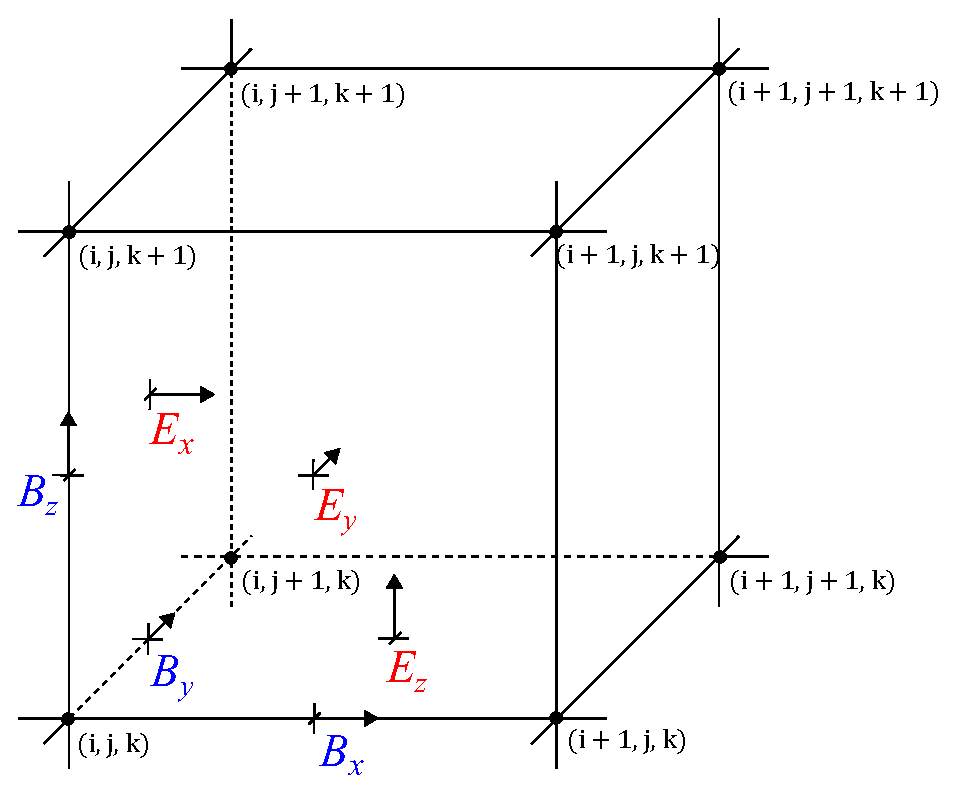
\includegraphics[width=0.355\paperwidth]{./img/YEE/yee.eps}
	\caption{Standard Cartesian Yee cell used for FDTD method}
	\label{3.1.1.14}
\end{figure}
Notice that this scheme achieves second-order accuracy in both, space and time. Discrete operators $ \left(\nabla^{+}\right) $ and $ \left(\nabla^{-}\right) $ used in \ref{3.1.1.6} - \ref{3.1.1.7} act on a scalar field $ f_{i j k} $ as follows,
\begin{equation}
\label{3.1.1.8}
\nabla^{+} f_{i j k} = \left(\frac{f_{i + 1,\: j,\: k} - f_{i,\: j,\: k}}{\Delta x}, \frac{f_{i,\: j + 1,\: k} - f_{i,\: j,\: k}}{\Delta y}, \frac{f_{i,\: j,\: k + 1} - f_{i,\: j,\: k}}{\Delta z} \right), 
\end{equation}
\begin{equation}
\label{3.1.1.9}
\nabla^{-} f_{i j k} = \left(\frac{f_{i,\: j,\: k} - f_{i - 1,\: j,\: k}}{\Delta x}, \frac{f_{i,\: j,\: k} - f_{i,\: j - 1,\: k}}{\Delta y}, \frac{f_{i,\: j,\: k} - f_{i,\: j,\: k - 1}}{\Delta z} \right).
\end{equation}
These operators have the following properties,
\begin{equation}
\label{3.1.1.10}
\nabla^{-} \cdot \nabla^{-} \times = \nabla^{+} \cdot \nabla^{+} \times = 0, \qquad \nabla^{-} \cdot \nabla^{+} = \nabla^{+} \cdot \nabla^{-} = \Delta^{\pm}.
\end{equation}
Symbol $ \Delta^{\pm} $ stands for the discrete Laplace operator in central differences,
\begin{equation}
\label{3.1.1.11}
\Delta^{\pm} f_{i, j, k} = \frac{f_{i - 1, j, k} + 2 f_{i, j, k} + f_{i + 1, j, k}}{\Delta x^{2}} + \frac{f_{i, j - 1, k} + 2 f_{i, j, k} + f_{i, j + 1, k}}{\Delta y^{2}} + \frac{f_{i, j, k - 1} + 2 f_{i, j, k} + f_{i, j, k + 1}}{\Delta z^{2}}.
\end{equation}

Before trying to find the solution of discretized Maxwell equations \ref{3.1.1.6} - \ref{3.1.1.7}, one must realize that this system of equations is not independent. In the three-dimensional case, there are eight first-order differential equations, but only six unknown vector components. Acting on the equations \ref{3.1.1.16} and \ref{3.1.1.7} by operators $ \left(\nabla^{-}\cdot\right) $ and $ \left(\nabla^{+}\cdot\right) $, respectively, one obtains
\begin{equation}
\label{3.1.1.12}
\frac{\nabla^{-} \cdot \vec{B}_{ijk}^{\,n + 1/2} - \nabla^{-} \cdot \vec{B}_{ijk}^{\,n - 1/2}}{\Delta t} = 0,
\end{equation}
\begin{equation}
\label{3.1.1.13}
\frac{\rho_{ijk}^{\,n + 1} - \rho_{ijk}^{\,n}}{\Delta t} + \nabla^{+} \cdot \vec{J}_{ijk}^{\,n + 1/2} = 0.
\end{equation}
It means that it is possible to solve only equations \ref{3.1.1.16} and \ref{3.1.1.7}, while the divergence equations \ref{3.1.1.6}, \ref{3.1.1.15} can be considered as the initial conditions. In this case, the continuity equation in finite differences (\ref{3.1.1.13}) have to be fulfilled.

\subsection{Particle and field weighting}
The particle weighting refers to the part of the code in which the charge and current densities are assigned to the discrete grid points from the continuous particle positions. After the fields are obtained, they are assigned back at the particles to calculate the Lorentz force. This step is called field weighting. It implies some form of interpolation.

First, have a look at the particle weighting. Charge density $ \rho\left(\vec{x}, t \right) $ and current density $ \vec{J}\left(\vec{x}, t \right) $ are given by the following integrals over the velocity space,
\begin{equation}
\label{3.1.2.1}
\rho\left(\vec{x}, t \right) = \sum_s q_s \int f_s \left(\vec{x}, \vec{v}, t \right) \mathrm{d} \vec{v}, \qquad \vec{J}\left(\vec{x}, t \right) = \sum_s q_s \int f_s \left(\vec{x}, \vec{v}, t \right) \vec{v} \, \mathrm{d} \vec{v}.
\end{equation}
The interpolation function is defined as
\begin{equation}
\label{3.1.2.2}
W_{i, j, k}\left(\vec{x}_{p}^{n}\right) =  \frac{1}{\Delta V}\int\limits_{\Omega} S_{x}\left(\vec{x} - \vec{x}_{p}^{n} \right) \mathrm{d} \vec{x}, \qquad \Delta V = \Delta x \Delta y \Delta z,
\end{equation}
where $ \Omega = \left\lbrace \vec{x} \in \mathbb{R}^{3} : \abs{x_{1} - x_{i, j, k}} \leq \Delta x/2 \wedge \abs{x_{2} - x_{i, j, k}} \leq \Delta y/2 \wedge \abs{x_{3} - x_{i, j, k}} \leq \Delta z/2 \right\rbrace $. Then the charge density $ \rho_{i, j, k}^{n} $ in the arbitrary grid point $ x_{i, j, k} $ and time level $ t^{n} $ is constructed as
\begin{equation}
\label{3.1.2.3}
\rho_{i, j, k}^{n} = \sum_{p} q_{p} W_{i, j, k}\left(\vec{x}_{p}^{n}\right), \qquad q_{p} = q_{s} N_{p},
\end{equation}
where the sum is taken over all computational particles.

By analogy, one could assign the current densities to the grid points using this interpolation function, but the discrete continuity equation for charge (\ref{3.1.1.13}) would not be satisfied exactly. In this case one have to solve Poisson's equation for correction of electric field or use one of the several numerical schemes for computing the current density satisfying the continuity equation, which are called charge conservation methods. In the next paragraph, the charge density decomposition method proposed by Esirkepov \cite{esirkepov} is described.

Due to linearity of the continuity equation (\ref{3.1.1.13}), it is sufficient to define the current density associated with the motion of a single computational particle,
\begin{equation}
\label{3.1.2.4}
\begin{split}
& \left(J_{x}\right)_{i+1,\: j,\: k}^{n} = \left(J_{x}\right)_{i,\: j,\: k}^{n} - q_{p} \left(v_{x}\right)_{p}^{n} \left(\Pi_{x}\right)_{i,\: j,\: k}^{n}, \\
& \left(J_{y}\right)_{i,\: j+1,\: k}^{n} = \left(J_{y}\right)_{i,\: j,\: k}^{n} - q_{p} \left(v_{y}\right)_{p}^{n} \left(\Pi_{y}\right)_{i,\: j,\: k}^{n}, \\
& \left(J_{z}\right)_{i,\: j,\: k+1}^{n} = \left(J_{z}\right)_{i,\: j,\: k}^{n} - q_{p} \left(v_{z}\right)_{p}^{n} \left(\Pi_{z}\right)_{i,\: j,\: k}^{n}.
\end{split}
\end{equation}
In accordance with continuity equation one can write
\begin{equation}
\label{3.1.2.7}
\left(\Pi_{x}\right)_{i,\: j,\: k}^{n} + \left(\Pi_{y}\right)_{i,\: j,\: k}^{n} + \left(\Pi_{z}\right)_{i,\: j,\: k}^{n} = W_{i, j, k}\left(\vec{x}_{p}^{n} + \vec{\tilde{x}}\right) - W_{i, j, k}\left(\vec{x}_{p}^{n}\right),
\end{equation}
where $ \vec{\tilde{x}} \in \mathbb{R}^{3} $ is the motion induced position shift of the computational particle in one simulation time step. Shift of the computational particle generates eight variants of interpolation functions,
\begin{equation}
\label{3.1.2.8}
\begin{split}
& W_{i, j, k}\left(\vec{x}_{p}^{n}\right), \quad W_{i, j, k}\left(\vec{x}_{p}^{n} + \tilde{x}_{1}\right), \quad W_{i, j, k}\left(\vec{x}_{p}^{n} + \tilde{x}_{2}\right), \quad W_{i, j, k}\left(\vec{x}_{p}^{n} + \tilde{x}_{3}\right), \\
& W_{i, j, k}\left(\vec{x}_{p}^{n} + \tilde{x}_{1} + \tilde{x}_{2}\right), \quad W_{i, j, k}\left(\vec{x}_{p}^{n} + \tilde{x}_{1} + \tilde{x}_{3}\right), \quad W_{i, j, k}\left(\vec{x}_{p}^{n} + \tilde{x}_{2} + \tilde{x}_{3}\right), \\
& W_{i, j, k}\left(\vec{x}_{p}^{n} + \tilde{x}_{1} + \tilde{x}_{2} + \tilde{x}_{3}\right).
\end{split}
\end{equation}
We assume that the vector $ \Pi_{i,\: j,\: k}^{\:n} $ is linearly dependent on the functions (\ref{3.1.2.8}). It turned out that only one linear combination exists.

Now, have a look at the field weighting. After calculating Maxwell equations at the grid points, it is necessary to assign electric and magnetic fields back at the particle positions. Recall the definition of interpolation function (\ref{3.1.2.2}). By analogy to the particle weighting, one can assign the components of electric field,
\begin{equation}
\begin{split}
& \left(E_{x}\right)_{p}^{n}  = \sum_{i, j, k} \left(E_{x}\right)^{n}_{i,\: j + 1/2,\: k + 1/2} W_{i,\: j + 1/2,\: k + 1/2} \left(\vec{x}_{p}^{n} \right), \\
& \left(E_{y}\right)_{p}^{n}  = \sum_{i, j, k} \left(E_{y}\right)^{n}_{i + 1/2,\: j,\: k + 1/2} W_{i + 1/2,\: j,\: k + 1/2} \left(\vec{x}_{p}^{n} \right), \\
& \left(E_{z}\right)_{p}^{n}  = \sum_{i, j, k} \left(E_{z}\right)^{n}_{i + 1/2,\: j + 1/2,\: k} W_{i + 1/2,\: j + 1/2,\: k} \left(\vec{x}_{p}^{n} \right),
\end{split}
\end{equation}
and the components of magnetic field,
\begin{equation}
\begin{split}
& \left(B_{x}\right)_{p}^{n}  = \sum_{i, j, k} \left(B_{x}\right)^{n}_{i + 1/2,\: j,\: k} W_{i + 1/2,\: j,\: k} \left(\vec{x}_{p}^{n} \right), \\
& \left(B_{y}\right)_{p}^{n}  = \sum_{i, j, k} \left(B_{y}\right)^{n}_{i,\: j + 1/2,\: k} W_{i,\: j + 1/2,\: k} \left(\vec{x}_{p}^{n} \right), \\
& \left(B_{z}\right)_{p}^{n}  = \sum_{i, j, k} \left(B_{z}\right)^{n}_{i,\: j,\: k + 1/2} W_{i,\: j,\: k + 1/2} \left(\vec{x}_{p}^{n} \right).
\end{split}
\end{equation} 
It is desirable to use the same interpolation function for both, density and force calculations, in order to eliminate a self-force and ensure conservation of momentum \cite{fehske}.


\subsection{Particle pusher}
The behavior of computational particles is controlled by the Newton-Lorentz equations. Since the particles can reach velocities near the velocity of light, it is necessary to perform relativistic generalization,
\begin{equation}
\label{3.2.4.1}
\vec{u}_{p} = \gamma \, \vec{v}_{p}, \qquad \gamma = \sqrt{1 + \left( \frac{\vec{u}_{p}}{c}\right)^{2}}.
\end{equation}
Assume that the electric and magnetic fields are interpolated from the grid points to the particles at the time level $ t^{n} $. Then the computational particle equations of motion to be integrated are
\begin{equation}
\label{3.2.4.2}
\diff[]{\vec{x}_{p}}{t} = \frac{\vec{u}_{p}}{\gamma}, \qquad \diff[]{\vec{u}_{p}}{t} = \frac{q_{s}}{m_{s}} \left(\vec{E}_{p} + \frac{\vec{u}_{p}}{\gamma} \times \vec{B}_{p} \right).
\end{equation}
To discretize equations of motion (\ref{3.2.4.2}) a time-centered leap-frog scheme is used. One obtains
\begin{equation}
\label{3.2.4.4}
\frac{\vec{x}_{p}^{\:n+1} - \vec{x}_{p}^{\:n}}{\Delta t} = \frac{\vec{u}_{p}^{\:n + 1/2}}{\gamma^{\:n+1/2}},
\end{equation}
\begin{equation}
\label{3.2.4.5}
\frac{\vec{u}_{p}^{\:n+1/2} - \vec{u}_{p}^{\:n-1/2}}{\Delta t} = \frac{q_{s}}{m_{s}} \left( \vec{E}_{p}^{\:n} + \frac{\vec{u}_{p}^{\:n+1/2} + \vec{u}_{p}^{\:n-1/2}}{2 \gamma^{\:n}} \times \vec{B}_{p}^{\:n} \right).
\end{equation}

Although these equations appear to be very simple, the solution is the most time-consuming part of the simulation, because they have to be solved for every single computational particle. Standard for particle pushing in plasma simulation PIC codes is elegant Boris method, which completely separates the effect of electric and magnetic fields \cite{birdsall}. Substitute
\begin{equation}
\label{3.2.4.6}
\vec{u}_{p}^{\:n-1/2} = \vec{u}_{p}^{\:-} - \frac{q_{s} \vec{E}_{p}^{\:n}}{m_{s}} \frac{\Delta t}{2}, \qquad \vec{u}_{p}^{\:n+1/2} = \vec{u}_{p}^{\:+} + \frac{q_{s} \vec{E}_{p}^{\:n}}{m_{s}} \frac{\Delta t}{2}
\end{equation}
into equation (\ref{3.2.4.5}), then the electric field cancels entirely,
\begin{equation}
\label{3.2.4.7}
\frac{\vec{u}_{p}^{\:+} - \vec{u}_{p}^{\:-}}{\Delta t} = \frac{q_{s}}{2 \gamma^{\:n} m_{s}} \left(\vec{u}_{p}^{\:+} + \vec{u}_{p}^{\:-}\right)\times \vec{B}_{p}^{\:n}. 
\end{equation}
Equation (\ref{3.2.4.7}) describes a rotation of vector $ \vec{u}_{p}^{\:-} $ to $ \vec{u}_{p}^{\:+} $ in one simulation time step $ \Delta t $. The angle $ \theta $ between vector $ \vec{u}_{p}^{\:-} $ and $ \vec{u}_{p}^{\:+} $ we expect to be $ \theta = \omega_{c} \Delta t $.

To implement the Boris method, first add half the electric impulse $ \vec{E}_{p}^{\:n} $ to $ \vec{u}_{p}^{\:n-1/2} $, then perform the full rotation by the angle $ \theta $, and finally, add another half the electric impulse $ \vec{E}_{p}^{n} $. From the basic geometry Boris derived following steps to obtain $ \vec{u}_{p}^{\:n + 1/2} $. From the first of equations (\ref{3.2.4.6}) express vector $ \vec{u}_{p}^{\:-} $,
\begin{equation}
\vec{u}_{p}^{\:-} = \vec{u}_{p}^{\:n-1/2} +  \frac{q_{s} \vec{E}_{p}^{\:n}}{m_{s}} \frac{\Delta t}{2}
\end{equation}
and construct an auxiliary vector $ \vec{u}_{p}\!' $, which is simultaneously perpendicular to $ \left(\vec{u}_{p}^{\:+} - \vec{u}_{p}^{\:-} \right) $ and to $ \vec{B}_{p}^{\:n} $,
\begin{equation}
\vec{u}_{p}\!' = \vec{u}_{p}^{\:-} + \vec{u}_{p}^{\:-} \times \vec{t}, \qquad \vec{t} = \frac{q_{s} \vec{B}_{p}^{\:n} \Delta t}{2 \gamma^{\:n} m_{s}}.
\end{equation}
Vector $ \vec{t} $ has to be logically parallel to $ \vec{B}_{p}^{n} $ with the length of $ \tan \left(\theta/2\right) \approx \theta/2 $ for small angles. Next, utilize the fact that the vector $ (\vec{u}_{p}\!' \times \vec{B}_{p}^{\:n}) $ is parallel to $ \left(\vec{u}_{p}^{\:+} - \vec{u}_{p}^{\:-} \right) $ and express $ \vec{u}_{p}^{\:+} $,
\begin{equation}
\vec{u}_{p}^{\:+} = \vec{u}_{p}^{\:-} + \vec{u}_{p}\!' \times \vec{s}, \qquad \vec{s} = \frac{2\vec{t}}{1 + t^2}.
\end{equation}
Here vector $ \vec{s} $ is parallel to $ \vec{B}_{p}^{n} $ and its length has to fulfill the condition $ \norm{\vec{u}_{p}^{\:+}} = \norm{\vec{u}_{p}^{\:-}} $. The transition from $ \vec{u}_{p}^{\:-} $ to $ \vec{u}_{p}^{\:+} $ can be written more clearly using the matrix,
\begingroup
\renewcommand*{\arraystretch}{1.8}
\begin{equation}
\vec{u}_{p}^{\:+} =  \begin{pmatrix}
  1 - s_{2}t_{2} - s_{3}t_{3} & s_{2}t_{1} + s_{3} & s_{3}t_{1} - s_{2} \\
  s_{1}t_{2} - s_{3} & 1 - s_{1}t_{1} - s_{3}t_{3} & s_{3}t_{2} + s_{1} \\
  s_{1}t_{3} + s_{2} & s_{2}t_{3} - s_{1} & 1 - s_{1}t_{1} - s_{2}t_{2}
 \end{pmatrix}
\vec{u}_{p}^{\:-}.
\end{equation}
\endgroup
Finally, substitute vector $ \vec{u}_{p}^{\:+} $ into the second from the equations (\ref{3.2.4.6}),
\begin{equation}
\vec{u}_{p}^{\:n+1/2} = \vec{u}_{p}^{\:+} + \frac{q_{s} \vec{E}_{p}^{\:n}}{m_{s}} \frac{\Delta t}{2}.
\end{equation}
The position of computational particle is advanced according to
\begin{equation}
\vec{x}_{p}^{\:n+1} = \vec{x}_{p}^{\:n} + \frac{\vec{u}_{p}^{\:n + 1/2}}{\gamma^{\:n + 1/2}} \Delta t, \qquad \gamma^{\:n + 1/2} = \sqrt{1 + \left(\frac{\vec{u}_{p}^{\:n + 1/2}}{c}\right)^{2}}.
\end{equation}




\subsection{Stability and accuracy}
\input{dat/3.1.4.tex}

\section{Code EPOCH}
The abbreviation EPOCH refers to an Extendable PIC Open Collaboration project \cite{bennett}. EPOCH is a multi-dimensional, relativistic, electromagnetic code designed for plasma physics simulations based on the PIC method. The code, which has been developed at University of Warwick, is written in FORTRAN and parallelized using MPI library. EPOCH is explicit and is able to achieve second-order accuracy. The entire core of the code uses SI units.

The main features include dynamic load balancing option for making optimal use of all processors when run in parallel, allowing restart on an arbitrary number of processors. The setup of EPOCH is controlled through a customizable input deck. An input deck is a text file which can be used to set simulation parameters for EPOCH without necessity to edit or recompile the source code. Most aspects of a simulation can be controlled, such as the number of grid points in the simulation domain, the initial distribution of particles and the initial electromagnetic field configuration. In addition, EPOCH has been written to add more modern features and to structure the code in such a way that the future expansion of the code may be made as easily as possible.

By default, EPOCH uses triangular particle shape functions with the peak located at the position of computational particle and a width of two cells, which provides relatively clean and fast solution. However, user can select higher order particle shape functions based on a spline interpolation by enabling compile-time option in the makefile.

The electromagnetic field solver uses a FDTD scheme with second order of accuracy. The field components are spatially staggered on a standard Cartesian Yee cell. The solver is directly based on the scheme derived by Hartmut Ruhl \cite{ruhl}. The particle pusher is relativistic, Birdsall and Landon type \cite{birdsall} and uses Villasenor and Buneman current weighting \cite{villasenor}.

EPOCH offers several types of boundary conditions for fields and particles, such as periodic, transmissive, reflecting and also Convolutional Perfectly Matched Layer (CPML) boundary conditions. Laser beams can be attached to arbitrary boundary via special boundary condition as well.

As a side project within this work, the code EPOCH has been instrumented to enable in situ diagnostics and visualization of the electromagnetic fields using ParaView Catalyst [source].
The increasing demands of the simulations need more data to be stored on a disk and analysed. However, the capabilities of computing environment which is responsible for transferring the data and communication have not grown up as rapid as the computational power. Dumping and processing of all the data calculated during the simulation would take too much time, so in practice this usually means that they are stored only at several time steps or at much coarser resolution than the original data. The rest is just discarded and the significant part of information may be potentially lost.

In situ visualization describes techniques where data can be visualized in real-time as it is generated during a simulation and without it being stored on a storage resource. By coupling the visualization and simulation, the data transfer bottleneck can be overcome. Furthermore, this approach allows scientists to monitor and interact with a running simulation, allowing for its parameters to be modified and allowing to immediately view the effects of these changes.

While a simulation is running, a user can see the size of the datasets that a simulation produces. But none of this data is physically stored on a storage system. The computationally expensive operations are carried out using ParaView’s graphical interface. So, the user can select data structures and analyze them in the same way as in post-processing, which requires the saving of datasets onto a file system. But there is one difference, the simulation is in progress so a user can observe the data as it is being generated. With Catalyst, it is also possible to pause the simulation or specify a break-point at a selected time step. This can be helpful if a user expects some interesting behavior of investigated phenomena or for identifying regions where numerical instability arises. For the implementation details, see Appendix - .

The main goal of this work has been to implement a solution that would enable to simulate tightly focused laser beams using simulation code EPOCH. This will be closer described in the following chapter.



%-------------------------------------------------------------------------------

\chapter{Tight-focusing of laser pulses}
The investigation of laser-matter interaction also involves exploring of specific themes of the ultra-relativistic regime, which requires extremely high intensities of the external field. These intensities, that are experimentally inaccessible at present, could be potentially achieved by tight-focusing and that would allow a broad spectrum of many multidisciplinary applications.

As mentioned in the previous chapter, various aspects of electromagnetic interaction are usually studied using sophisticated numerical simulation codes. Vast majority of these codes, however, use a paraxial approximation (closer described in chapter 1) to prescribe the laser fields at the boundaries, and afterwards, a field solver guides the beam across the simulation domain. As already mentioned, the paraxial approximation is valid only if the angular spectrum of laser pulse is sufficiently narrow, therefore it is not possible to simulate tightly focused laser beams using this approach. As might be seen later, paraxial approximation in this case leads to a distorted field profiles which have strong impact on the results of laser-matter interaction.

Several interesting solutions, how to simulate strongly focused beams, have been already proposed [source]. Within this work, a simple and efficient algorithm for a Maxwell consistent calculation of the electromagnetic fields at the boundaries of the computational domain [source] (also called laser boundary conditions) has been used and implemented into the PIC code EPOCH [source]. Note, that this algorithm is able to describe laser beams with arbitrary shape.

\section{Laser boundary conditions}
In this section, another mathematical description of a focused laser beam based on a rigorous solution of the wave equation \ref{1.34} is presented. The following calculations are reproduced from the work of Illia Thiele et al. \cite{Thiele2016}. Assume that the laser beam propagates in vacuum without external sources along the z-axis of the Cartesian coordinate system. The wave equation \ref{1.34} in temporal Fourier space has the following form,
\begin{equation}
\label{4.1}
\laplace{\hat{\vec{E}}} \left(\vec{r}, \omega \right) + \frac{\omega^2}{c^2} \hat{\vec{E}} \left(\vec{r}, \omega \right) = 0,
\end{equation}
where the hat symbol placed on the top of a variable denotes the Fourier transform with respect to time. Next, one shall perform a spatial Fourier transform of \ref{4.1} with respect to transverse coordinates $ \vec{r_\bot} $ only,
\begin{equation}
\label{4.2}
\left(- k^2_x - k^2_y + \diffp[2]{}{z} \right) \bar{\vec{E}} \left(k_x, k_y, z, \omega \right) + \frac{\omega^2}{c^2} \bar{\vec{E}} \left(k_x, k_y, z, \omega \right) = 0,
\end{equation}
where the bar symbol placed on the top of a variable denotes the Fourier transform with respect to time and spatial transverse coordinates. The equation \ref{4.2} can be simplified as follows,
\begin{equation}
\label{4.3}
k^2_z \left(\vec{k}_\bot, \omega \right) \bar{\vec{E}}(\vec{k}_\bot, z, \omega) + \diffp[2]{}{z} \bar{\vec{E}} \left(\vec{k}_\bot, z, \omega \right) = 0.
\end{equation}
where $ k_z \left(\vec{k}_\bot, \omega \right) = \sqrt{-\vec{k}_\bot^2 + \omega^2/c^2} $ and $ \vec{k}_\bot = (k_x, k_y)^{\mathrm{T}} $. The fundamental solution of the equation \ref{4.3} consists of the forward $ (+) $ and backward $ (-) $ propagating waves,
\begin{equation}
\label{4.4}
\bar{\vec{E}}^{\pm} \left(\vec{k}_\bot, z, \omega \right) = \bar{\vec{E}}_{0}^{\pm} \left(\vec{k}_\bot, \omega \right) \e^{\pm \i k_z \left(\vec{k}_\bot, \omega \right) \left(z - z_0 \right)}.
\end{equation}
Where $ \bar{\vec{E}}_{0}^{\pm}\left(\vec{k}_\bot, \omega \right) $ is the electric laser field at some plane $ z = z_0 $. It might be clearly seen, that only two out of six vector components of the electric and magnetic fields are independent, therefore one may prescribe for example the transverse components $ \bar{\vec{E}}_{0, \bot}^{\pm}\left(\vec{k}_\bot, \omega \right) $ at the plane $ z = z_0 $ and all other components can be derived from the Maxwell's equations \ref{1.1}, \ref{1.3},
\begin{equation}
\label{4.5}
\bar{\vec{E}}^{\pm}_{\bot} \left(\vec{k}_\bot, z, \omega \right) = \bar{\vec{E}}^{\pm}_{0, \bot} \left(\vec{k}_\bot, \omega \right) \e^{\pm \i k_z \left(\vec{k}_\bot, \omega \right) \left(z - z_0 \right)},
\end{equation}
\begin{equation}
\label{4.6}
\bar{E}^{\pm}_z \left(\vec{k}_\bot, z, \omega \right) = \mp \frac{\vec{k}_\bot \cdot \bar{\vec{E}}^{\pm}_{\bot}(\vec{k}_\bot, z, \omega)}{k_z \left(\vec{k}_\bot, \omega \right)},
\end{equation}
\begin{equation}
\label{4.7}
\bar{\vec{B}}^{\pm}_{\bot} \left(\vec{k}_\bot, z, \omega \right) = \frac{1}{\omega k_z \left(\vec{k}_\bot, \omega \right)} \mathbb{R}^{\pm} \left(\vec{k}_\bot, \omega \right) \bar{\vec{E}}^{\pm} \left(\vec{k}_\bot, z, \omega \right),
\end{equation}
where
\begingroup
\renewcommand*{\arraystretch}{1.7}
\begin{equation}
\label{4.8}
\mathbb{R}^{\pm} \left(\vec{k}_\bot, \omega \right) =  \begin{pmatrix}
\mp k_x k_y & \mp \left[ k_z^2 \left(\vec{k}_\bot, \omega \right) + k_y^2 \right] & 0 \\
\pm \left[ k_z^2 \left(\vec{k}_\bot, \omega \right) + k_x^2 \right] & \pm k_x k_y & 0 \\
- k_y k_z \left(\vec{k}_\bot, \omega \right) & - k_x k_z \left(\vec{k}_\bot, \omega \right) & 0
\end{pmatrix}.
\end{equation} 
\endgroup

Analogically, one could solve the wave equation for the magnetic field \ref{1.35}, prescribe two transverse components of $ \bar{\vec{B}}_{0, \bot}^{\pm}\left(\vec{k}_\bot, \omega \right) $ at the plane $ z = z_0 $ and afterwards calculate all other fields using Maxwell's equations \ref{1.2}, \ref{1.4}. The complete proof, that the fields \ref{4.5} - \ref{4.7} are consistent with the Maxwell's equations in vacuum \ref{1.1} - \ref{1.4} can be found in the original paper \cite{Thiele2016}.

Note that for $ k_\bot^2 > \omega^2/c^2 $, $ k_z \left(\vec{k}_\bot, \omega \right) $ becomes imaginary and equation \ref{4.4} describes evanescent waves that are unphysical in free space. Thus the Fourier spectrum of laser waves has to be filtered in the transverse Fourier space. On the other hand, if the spatial Fourier spectrum contains only components with $ k_\bot^2 \ll \omega^2/c^2 $, then $ k_z \left(\vec{k}_\bot, \omega \right) $ can be approximated using the first few terms of a Taylor series,
\begin{equation}
\label{4.9}
k_z \left(\vec{k}_\bot, \omega \right) \approx \frac{\abs{\omega}}{c} - \frac{c}{2 \abs{\omega}} k_\bot^2.
\end{equation}
Note that by plugging \ref{4.9} into equations \ref{4.5} - \ref{4.7} one gets the paraxial approximation.

In the last part of this section, the practical algorithm for implementation of the boundary conditions based on the previously derived solution of the Maxwell's equations is presented. Assume that the laser beam propagates in a forward direction along the z-axis. In the beginning, it is necessary to prescribe the electric laser field $ \vec{E}_{0, \bot} (\vec{r}_{\bot}, t) $ in the plane $ \mathcal{P} $ at $ z = z_0 $. Note, that it can be defined by arbitrary function of space and time. The goal is then to find the fields $ \vec{E}_{\mathrm{B}} (\vec{r}_{\bot}, t) $ and $ \vec{B}_{\mathrm{B}} (\vec{r}_{\bot}, t) $ at the corresponding boundary $ z = z_\mathrm{B} $.

Consider that the transverse part of simulation domain is made of equidistant rectangular grid described by $ x^{i} $, $ y^{j} $, where $ i, j \in \left\lbrace 1, \ldots, N_{x, y} \right\rbrace $, and the grid steps $ \delta x $, $\delta y $. The simulation time $ t^{n} $, where $ n \in \left\lbrace 1, \ldots, N_{t} \right\rbrace $, is also divided into equidistant time steps of size $ \delta t $.

The algorithm allows to calculate fields $ \vec{E}_{\mathrm{B}}^{ij} (t) $ and $ \vec{B}_{\mathrm{B}}^{ij} (t) $ for any given time $ t $ from the interval $ \left[ t^{1} - \frac{z_\mathrm{B} - z_0}{c}, t^{N_t} - \frac{z_\mathrm{B} - z_0}{c} \right] $. In order to preserve clarity, the algorithm below is given in the exact form as in the original paper \cite{Thiele2016}.

\begin{enumerate}
	\item Calculate $ \hat{\vec{E}}_{0, \bot}^{ijn} $ via discrete Fourier transforms in time:
	\begin{equation}
	\omega^n = \frac{2 \pi}{N_t \delta t} \left( -\frac{N_t}{2} + n \right),
	\end{equation}
	\begin{equation}
	\hat{\vec{E}}_{0, \bot}^{ijn} = \frac{\delta t}{2 \pi} \sum_{l=1}^{N_t} \vec{E}_{0, \bot}^{ijl} \e^{\i \omega^n t^l}, \quad n \in \left\lbrace 1, \dots, N_t \right\rbrace.
	\end{equation}
	\item Calculate $ \bar{\vec{E}}_{0, \bot}^{ijn} $ via two-dimensional discrete Fourier transforms in transverse space:
	\begin{equation}
	k_x^i = \frac{2 \pi}{N_x \delta x} \left( - \frac{N_x}{2} + i\right), \quad k_y^j = \frac{2 \pi}{N_y \delta y} \left( - \frac{N_y}{2} + j\right),
	\end{equation}
	\begin{equation}
	\bar{\vec{E}}_{0, \bot}^{ijn} = \frac{\delta x \delta y}{(2 \pi)^2} \sum_{l, m = 1}^{N_x, N_y} \hat{\vec{E}}_{0, \bot}^{lmn} \e^{- \i \: \left(k_x^i x^l + k_y^j y^m \right)}, \quad i, j \in \left\lbrace 1, \dots, N_{x, y} \right\rbrace.
	\end{equation}
	\item Calculate transverse electric field components at the boundary $ z = z_\mathrm{B} $:
	\begin{equation}
	k_z^{ijn} = \Re \sqrt{\frac{(\omega^n)^2}{c^2} - (k_x^i)^2 - (k_y^j)^2},
	\end{equation}
	\begin{equation}
	\bar{\vec{E}}_{\mathrm{B}, \bot}^{ijn} =
	\begin{cases} \bar{\vec{E}}_{0, \bot}^{ijn} \e^{\i k_z^{ijn}(z_\mathrm{B} - z_0)} & \text{for} \ k_z^{ijn} > 0 \\ 0 & \text{for} \ k_z^{ijn} = 0 \end{cases}.
	\end{equation}
	\item Calculate longitudinal electric field components at the boundary $ z = z_\mathrm{B} $:
	\begin{equation}
	\bar{E}_{\mathrm{B}, z}^{ijn} = \begin{cases} -\frac{k_x^i \bar{E}_{\mathrm{B}, x}^{ijn} + k_y^j \bar{E}_{\mathrm{B}, y}^{ijn}}{k_z^{ijn}} & \text{for} \ k_z^{ijn} > 0 \\ 0 & \text{for} \ k_z^{ijn} = 0 \end{cases}.
	\end{equation}
	\item Calculate the magnetic field at the boundary $ z = z_\mathrm{B} $:
	\begingroup
	\renewcommand*{\arraystretch}{1.7}
	\begin{equation}
	\mathbb{R}^{ijn} =  \begin{pmatrix}
	-k_x^i k_y^j & (k_x^i)^2 - (\omega^n)^2/c^2 \\
	(\omega^n)^2/c^2 - (k_y^j)^2 & k_x^i k_y^j \\
	-k_y^j k_z^{ijn} & k_x^i k_z^{ijn} 
	\end{pmatrix},
	\end{equation} 
	\endgroup
	\begin{equation}
	\bar{\vec{B}}_{\mathrm{B}}^{ijn} = \begin{cases} (\omega^n k_z^{ijn})^{-1} \mathbb{R}^{ijn} \bar{\vec{E}}_{\mathrm{B}, \bot}^{ijn} & \text{for} \ k_z^{ijn} > 0 \\ 0 & \text{for} \ k_z^{ijn} = 0 \end{cases}.
	\end{equation}
	\item Calculate $ \hat{\vec{E}}_{\mathrm{B}}^{ijn} $, $ \hat{\vec{B}}_{\mathrm{B}}^{ijn} $ via two-dimensional inverse discrete Fourier transforms:
	\begin{equation}
	\hat{\vec{E}}_{\mathrm{B}}^{ijn} = \frac{(2 \pi)^2}{N_x N_y \delta x \delta y} \sum_{l, m = 1}^{Nx, Ny} \bar{\vec{E}}_{\mathrm{B}}^{lmn} \e^{\i(k_x^l x^i + k_y^m y^j)},
	\end{equation}
	\begin{equation}
	\hat{\vec{B}}_{\mathrm{B}}^{ijn} = \frac{(2 \pi)^2}{N_x N_y \delta x \delta y}  \sum_{l, m = 1}^{Nx, Ny} \bar{\vec{B}}_{\mathrm{B}}^{lmn} \e^{\i(k_x^l x^i + k_y^m y^j)}.
	\end{equation}
	\item Calculate $ \vec{E}_{\mathrm{B}}^{ij}(t) $, $ \vec{B}_{\mathrm{B}}^{ij}(t) $ for any given time $ t \in [t^{1} - \frac{z_{\mathrm{B}} - z_{0}}{c}, t^{N_{t}}  - \frac{z_{\mathrm{B}} - z_{0}}{c}] $.
	\begin{equation}
	\vec{E}_{\mathrm{B}}^{ij} (t) = \frac{2 \pi}{N_t \delta t} \sum_{n = 1}^{N_t} \hat{\vec{E}}_{\mathrm{B}}^{ijn} \e^{-\i \omega^n t},
	\end{equation}
	\begin{equation}
	\vec{B}_{\mathrm{B}}^{ij} (t) = \frac{2 \pi}{N_t \delta t} \sum_{n = 1}^{N_t} \hat{\vec{B}}_{\mathrm{B}}^{ijn} \e^{-\i \omega^n t}.
	\end{equation}
\end{enumerate}

\section{Implementation}
One of the main goals of this work has been to implement the algorithm mentioned in the previous section, to evaluate its correctness in several test simulations and finally, to exploit resulting implementation for simulations of tightly focused Gaussian beams in laser-matter interaction. The main requirement on implementation was fast integration with the 2D version of particle-in-cell simulation code EPOCH \cite{bennett}. For this reason, several possible solutions have been taken into account.

The final decision was to create a static library, which will be able to compute desired quantities and will provide functions for communication with the main simulation code. The essential advantage is that it could be basically linked with any laser-plasma simulation code. Also, since it is necessary to call only two additional functions, the instrumentation will be fast, easy and the main simulation code will not be excessively disturbed. Furthermore, the implementation itself come with the CMake \cite{Cmake2012} support, which simplify the compilation process using platform and compiler independent configuration files.

The library has been written in C++ language in the object-oriented style, so the algorithm can be easily extended to the three dimensional geometry. In order to speedup the whole underlying computation, the algorithm has been parallelized using hybrid techniques. The time domain has been decomposed into the stripes corresponding to individual computational processes, the communication between these processes is ensured by MPI library \cite{MPI1994}. Furthermore, the computationally most expensive cycles are parallelized using OpenMP implementation of multi-threading \cite{OpenMP1998}. Later on, the speedup and parallel scaling performance will be briefly discussed.

Fourier transforms form the core of the computational process and their performance is crucial for the overall performance of the code. For this reason, many currently available libraries have been considered. Eventually, the Fourier transforms in the algorithm can be computed using FFTW \cite{Frigo1998} library, Intel$ ^{\scriptsize \textregistered} $ MKL \cite{MKL2009} library or it is also possible to directly evaluate the formulas without using any additional library. User specifies his option before the compilation of the code. Regarding both libraries, a threaded versions of 1D in-place complex fast Fourier transforms have been used throughout the code. According to several measures, there is no significant difference between the speed of both libraries. On Intel$ ^{\scriptsize \textregistered} $ architectures, the MKL library \cite{MKL2009} has slightly better performance though.

One potential bottleneck could happen during the computation of spatial Fourier transforms since the arrays with spatial data are decomposed into different processes. The cluster versions of functions performing the Fourier transforms have been tested, however they did not bring any significant speedup. The reason is as follows. They require to have the global array in memory and use its own distribution which involves overlapping. Since the size of global arrays is usually not so large and since it is necessary to perform a lot of different Fourier transforms, the majority of computational time is spent rather for communication, mainly if many of computational cores are used.

This issue has been solved by gathering the data on master process, performing the Fourier transforms in space by only one processor and scattering the data back to corresponding processes. This is the reason why the code does not scale well, however, the time to compute all desired quantities is in most cases negligible in comparison with the time required by the main simulation cycle. Nevertheless, this could be a suggestion for future improvement.

Since it is necessary to compute the whole time evolution of the laser field at boundary for each grid point before the simulation starts, the resulting amount of data can be significantly large and does not have to fit in a computer RAM. Thus, it is inevitable to dump the data into a file, which will be then accessed by the main simulation code. Due to the performance purposes, each computational process stores its data into a shared file with corresponding offset and in binary coding. Therefore, the output operations are as fast as possible and save the storage resources. Library then provide a function which allows to seek an arbitrary position in a file. This function is then called each time step of the main simulation loop to fill the laser source arrays with all the relevant data. This way of accessing data does not cause any significant slowdown or memory overhead.

The EPOCH \cite{bennett} code require only transverse components of the laser electric field, all other quantities are computed by the FDTD solver \cite{ruhl}. The implementation of the library allows full connection with EPOCH \cite{bennett}. In practice, if user wants to simulate tight-focusing, it is necessary to enable the corresponding flag as a compile-time option and then to specify all required parameters in the input file. The code then automatically computes all necessary data. It works generally regardless the number of lasers in the simulation or boundaries that they are attached to.

The current version of library does not work for obliquely incident laser pulses, because in this case one cannot exploit the advantage of an efficient computation with fast Fourier transforms. However, the code allows to compute the laser fields at boundary by evaluating Fourier integrals directly, so it could be easily extended. Second, it is at the moment possible to simulate only Gaussian laser pulses. However, user can prescribe its own shape and position of the beam in focal plane by modifying corresponding part of the code.

Several most important data structures, functions and methods that form the core of the library for tight-focusing can be seen in appendix B.

\section{Evaluation}
\floatsetup[figure]{style=plain, subcapbesideposition=top}
\begin{figure}[h!]
	\centering
	\sidesubfloat[]{{\includegraphics[width=0.44\linewidth]{./img/parax/Ey_focus.pdf}}}
	\hspace{2mm}
	\sidesubfloat[]{{\includegraphics[width=0.44\linewidth]{./img/parax/Ex_focus.pdf}}}\\
	\sidesubfloat[]{{\includegraphics[width=0.44\linewidth]{./img/lbcs/Ey_focus.pdf}}}
	\hspace{2mm}
	\sidesubfloat[]{{\includegraphics[width=0.44\linewidth]{./img/lbcs/Ex_focus.pdf}}}
	\caption{Transverse ($ E_{y} $) and longitudinal ($ E_{x} $) electric laser field components captured at the time step of their maximal intensity at the focal spot. The cases \textbf{(a)}, \textbf{(b)} correspond to the laser pulse initialized using the paraxial approximation, whilst \textbf{(c)}, \textbf{(d)} come from the simulation where the beam at the boundary is given by the Maxwell consistent approach. In the case of paraxial approximation, both components reveal strong distortions and asymmetry, their focal spot is located about $ \mathrm{1 \lambda} $ closer to the left boundary than specified and the corresponding amplitude is significantly lower. The laser has been attached to the left hand side boundary.}
	\label{fig:1}
\end{figure}

To evaluate the correctness of the algorithm presented in the previous section of this chapter as well as to demonstrate the drawbacks of the paraxial approximation, several test simulations in 2D geometry have been performed. In the following text, a two limit cases are presented. The first pair of simulations employs tightly focused Gaussian laser beam with the size at focus comparable with the center laser wavelength, whilst the second one shows the case of the Gaussian beam with the size at focus one order of magnitude larger than the center laser wavelength, where both approaches should return identical results. Note, that all the simulations have been computed using 2D version of PIC code EPOCH [source] instrumented with library for tight-focusing.

\floatsetup[figure]{style=plain, subcapbesideposition=top}
\begin{figure}[h!]
	\centering
	\sidesubfloat[]{{\includegraphics[width=0.4\linewidth]{./img/parax/Ey_focus_trans.pdf}}}
	\hspace{2mm}
	\sidesubfloat[]{{\includegraphics[width=0.4\linewidth]{./img/parax/Ey_focus_long.pdf}}}\\
	\sidesubfloat[]{{\includegraphics[width=0.4\linewidth]{./img/lbcs/Ey_focus_trans.pdf}}}
	\hspace{2mm}
	\sidesubfloat[]{{\includegraphics[width=0.4\linewidth]{./img/lbcs/Ey_focus_long.pdf}}}
	\caption{Transverse \textbf{(a)}, \textbf{(c)} and longitudinal \textbf{(b)}, \textbf{(d)} slices of the transverse electric laser field ($ E_{y} $) at the time step when it reaches maximal intensity at the focal spot. The cases \textbf{(a)}, \textbf{(b)} correspond to the laser pulse initialized using the paraxial approximation, whilst \textbf{(c)}, \textbf{(d)} come from the simulation where the beam at the boundary is given by the Maxwell consistent approach. In the case of paraxial approximation, one can clearly see strong side-wings in the spatial beam profile \textbf{(a)} as well as the asymmetry of the field in the longitudinal line-out \textbf{(b)}.}
	\label{fig:2}
\end{figure}

The simulation of a tightly focused Gaussian beam is considered first. The p-polarized laser pulse with center wavelength $ \lambda = 1 \ \mathrm{\mu m} $ propagates from left hand side boundary to the right. Its duration has been chosen to $ \tau = 20 \ \mathrm{fs} $ in FWHM and amplitude $ E_0 = 1 \cdot 10^{15} \ \mathrm{V/m} $. The beam waist $ w_0 = 0.7 \ \mathrm{\mu m} $ is shorter than the laser wavelength, which implies that non-negligible parts of $ \bar{\vec{E}}_{0, \bot}(k_x, \omega) $ are evanescent. The focus is located at a distance $ x = 8 \ \mathrm{\mu m} $ from the boundary that the laser is attached to.

The size of the simulation domain is $ 16 \lambda \times 48 \lambda $, with 100 cells per laser wavelength in both directions, thus $ \Delta x = \Delta y = \lambda/100 = 10 \ \mathrm{nm} $. The simulation time step is chosen to satisfy the CFL condition [source] $ \Delta t = 0.95 \sqrt{2} \lambda/ 100 c \approx 0.05 \ \mathrm{fs} $ and the whole simulation time is $ t = 150 \ \mathrm{fs} $. The pulse propagates in vacuum in order to get rid of all effects that could be potentially caused by plasma. All the simulation parameters can be found in the attached input files in the appendix A.

\floatsetup[figure]{style=plain, subcapbesideposition=top}
\begin{figure}[h!]
	\centering
	\sidesubfloat[]{{\includegraphics[width=0.44\linewidth]{./img/lbcs/Ey_boundary_time.pdf}}}
	\hspace{2mm}
	\sidesubfloat[]{{\includegraphics[width=0.44\linewidth]{./img/lbcs/Ex_boundary_time.pdf}}}
	\caption{The time evolution of transverse ($ E_{y} $) \textbf{(a)} and longitudinal ($ E_{x} $) \textbf{(b)} electric laser field components at the boundary that the laser is attached to. Both components has been calculated according to the Maxwell consistent approach.}
	\label{fig:3}
\end{figure}

\begin{figure}[h!]
	\centering
	\sidesubfloat[]{{\includegraphics[width=0.45\linewidth]{./img/lbcs/divergence.pdf}}}
	\hspace{2mm}
	\sidesubfloat[]{{\includegraphics[width=0.43\linewidth]{./img/parax/focus_shift.pdf}}}
	\caption{\textbf{(a)} Graph of the spot size parameter $ w(x) $ of the beams with $ w_0 = 1 \: \lambda $ and $ 0.5 \: \lambda $ calculated using Maxwell consistent approach. From the plotted lines, one can roughly estimate the beam divergence angle $ \Theta $. The divergence angles for both beams are surprisingly in a good accordance with the formula for divergence angles of corresponding Gaussian beams. \textbf{(b)} Dependency of the absolute focal point shift on the beam waist $ w_0 $ for the laser beam initialized using the paraxial approximation. One can see sharp increase of the error for $ w_0 < \lambda $. In both cases, values have been dumped at discrete time intervals and interpolated.}
	\label{fig:7}
\end{figure}

\floatsetup[figure]{style=plain, subcapbesideposition=top}
\begin{figure}[h!]
	\centering
	\sidesubfloat[]{{\includegraphics[width=0.44\linewidth]{./img/lbcs/Ey_boundary_trans.pdf}}}
	\hspace{1mm}
	\sidesubfloat[]{{\includegraphics[width=0.44\linewidth]{./img/lbcs/Ey_boundary_long.pdf}}}
	\caption{Transverse \textbf{(a)} and longitudinal \textbf{(b)} slice of the transverse electric laser field ($ E_{y} $) when it reaches its maximal intensity at the front (blue) and rear (red) boundary. The results come from the simulation where the laser beam at the boundary has been calculated using the Maxwell consistent approach. For better comparison, the field at the rear boundary in \textbf{(b)} has been horizontally flipped. The exact match between the field shapes at a different time steps of simulation proves the correctness of the laser beam propagation.}
	\label{fig:4}
\end{figure}

In the following paragraph, the results of the first simulation are discussed in more details. Fig. \ref{fig:1} shows the transverse and longitudinal electric field components at their maximal intensity at focus for two cases. First, for the laser beam which has been initialized using the paraxial approximation (fig. \ref{fig:1} - a, b), i.e. the electric field at the boundary is given by the equation \ref{1.50}, and second, according to the approach consistent with the Maxwell's equations (fig. \ref{fig:1} - c, d). In the case of paraxial approximation, one can clearly see strong distortions and asymmetry in the shape of both electric field components. In addition, the focus location is shifted about $ 1 \ \mathrm{\mu m} $ closer to the left boundary and the corresponding amplitude at focus is less than half the required value. In contrast, the fields produced by the simulation using Maxwell consistent calculation of laser fields at boundary are symmetric with respect to the focal spot and without any distortions. Furthermore, the focus location as well as the amplitude fulfills the initial requirements precisely.

Fig. \ref{fig:2} shows transverse and longitudinal slices of transverse electric field component at focus for the case of the laser beam initialized using the paraxial approximation (fig. \ref{fig:2} - a, b) as well as for the case where the beam at the boundary is given by the Maxwell consistent approach (fig. \ref{fig:2} - c, d). For the case of paraxial approximation, one can clearly see the asymmetry of the field shape in the longitudinal slice (fig. \ref{fig:2} - b), which consequently leads to a decrease of the amplitude at focus and to the strong side-wings in the spatial beam profile, as might be better seen from the transverse slice (fig. \ref{fig:2} - a). On the other hand, Maxwell consistent approach calculates fields of perfect symmetry with respect to the focal spot (fig. \ref{fig:2} - c) and no side-wings or distortions are present (fig. \ref{fig:2} - d).

\begin{figure}[h!]
	\centering
	\sidesubfloat[]{{\includegraphics[width=0.445\linewidth]{./img/lbcs/amplitude.pdf}}}
	\hspace{2mm}
	\sidesubfloat[]{{\includegraphics[width=0.435\linewidth]{./img/lbcs/intensity.pdf}}}
	\caption{\textbf{(a)} Graph of the transverse ($ E_{y} $) electric laser field amplitude with respect to the distance from the focal spot. The values on vertical axis are given in a percentage of the amplitude at focus $ E_{y, 0} $. \textbf{(b)} Graph of the maximal instantaneous laser intensity with respect to the distance from focal spot. The values on vertical axis are given in a percentage of the laser intensity at focus $ I_{0} $. In both cases, values have been computed using the Maxwell consistent approach, dumped at discrete time intervals and interpolated.}
	\label{fig:8}
\end{figure}

\floatsetup[figure]{style=plain, subcapbesideposition=top}
\begin{figure}[h!]
	\centering
	\sidesubfloat[]{{\includegraphics[width=0.45\linewidth]{./img/parax/Ey_focus_5mic.pdf}}}
	\hspace{2mm}
	\sidesubfloat[]{{\includegraphics[width=0.44\linewidth]{./img/parax/Ex_focus_5mic.pdf}}}\\
	\sidesubfloat[]{{\includegraphics[width=0.44\linewidth]{./img/lbcs/Ey_focus_5mic.pdf}}}
	\hspace{2mm}
	\sidesubfloat[]{{\includegraphics[width=0.43\linewidth]{./img/lbcs/Ex_focus_5mic.pdf}}}
	\caption{Transverse ($ E_{y} $) and longitudinal ($ E_{x} $) electric laser field components captured at the time step of their maximal intensity at the focal spot. The cases \textbf{(a)}, \textbf{(b)} correspond to the laser pulse initialized using the paraxial approximation, whilst \textbf{(c)}, \textbf{(d)} come from the simulation where the beam at the boundary is given by the Maxwell consistent approach. The size of the focus has been chosen to be one order of the magnitude larger than the center laser wavelength. One can clearly see, that there is no significant difference between the shapes of the electric field components.}
	\label{fig:5}
\end{figure}

\floatsetup[figure]{style=plain, subcapbesideposition=top}
\begin{figure}[h!]
	\centering
	\sidesubfloat[]{{\includegraphics[width=0.44\linewidth]{./img/parax/Ey_focus_trans_comparison.pdf}}}
	\hspace{2mm}
	\sidesubfloat[]{{\includegraphics[width=0.44\linewidth]{./img/parax/Ey_focus_long_comparison.pdf}}}
	\caption{Transverse \textbf{(a)} and longitudinal \textbf{(b)} slices of the transverse electric laser field ($ E_{y} $) at the time step when it reaches maximal intensity at focus. Red lines correspond to the laser pulse initialized using the paraxial approximation, whilst blue lines come from the simulation where the beam at the boundary is calculated by the Maxwell consistent approach (LBCS). The size of the focus has been chosen to be one order of magnitude larger than the center laser wavelength. In the case of paraxial approximation, the focus is slightly shifted closer to the left boundary \textbf{(b)}, otherwise the size of the focus as well as the amplitude is correct for both cases \textbf{(a)}.}
	\label{fig:6}
\end{figure}

In fig. \ref{fig:3} one can look through the time evolution of transverse (fig. \ref{fig:3} - a) and longitudinal (fig. \ref{fig:3} - b) electric field components at the boundary as computed using the Maxwell consistent approach. Note that one must chose carefully the transverse size of the domain, since the beam width at boundary may be much larger than at focus because of a diffraction. To estimate the beam width at the boundary, one has to know the beam divergence angle $ \Theta $. In fig. \ref{fig:7} - a, one can find a graph of the spot size parameter $ w $ as calculated using the Maxwell consistent approach for the beams focused to $ w_0 = 1 \ \lambda $ and $ 0.5 \ \lambda $. From the plotted lines, one can roughly estimate the beam divergence angle $ \Theta $. For the beam focused to $ w_0 = 1 \ \lambda $, the beam divergence angle has been around $ \Theta = 18.2 ^{\circ} $ which is almost identical value as for the Gaussian beam of the same parameters. For the beam with $ w_0 = 0.5 \ \lambda $ the divergence has been estimated to $ \Theta = 32.9 ^{\circ} $, while the Gaussian beam with the same size at focus has divergence $ \Theta = 36.5 ^{\circ} $. Consequently, in spite of the fact that the divergence of the tightly focused beams calculated using the Maxwell consistent approach is a little bit lower, both approaches are in quite a good accordance regarding this parameter and one can use the angle $ \Theta $ given by the equation \ref{1.38} as a rough estimate even for tight-focusing.

To evaluate a correctness of the propagation of the beam prescribed using the Maxwell consistent approach, several criteria has been defined. The correctness of the amplitude and beam waist as well as the right focus location has already been verified. Additional criteria has been set on a beam symmetry. In fig. \ref{fig:4}, one can find a comparison of the transverse electric laser field component when it achieves its maximal intensity at front and rear boundary. One can clearly see the exact match between the field shapes at different time steps of the simulation in transverse (fig. \ref{fig:4} - a) and longitudinal (fig. \ref{fig:4} - b) slices. Moreover, all the aforementioned criteria has been fulfilled also in other simulations with different input parameters that are not presented here. Consequently, these observations prove the correctness of the simulation at least for the tightly focused Gaussian laser beams.

In fig. \ref{fig:7} - b, one may find the estimate of the absolute focal point shift with respect to the prescribed position of the beam waist. The interpolated values come from the simulations where the laser beam has been initialized using paraxial approximation. One can clearly see the sharp increase of the error for $ w_0 < \lambda $. On the other hand, for $ w_0 = 5 \ \lambda $ the shift is around $ 0.2 \ \lambda $ which is negligible in comparison with the Rayleigh range.

In fig. \ref{fig:8} - a, one can see the amplitude of the transverse electric laser field with respect to the distance from the focal spot calculated using Maxwell consistent approach. This could be particularly useful for experiments since it is not always easy to focus the beam onto the target surface perfectly. Sometimes, one might be more interested in the laser intensity rather than the amplitude of the electric field. For this reason, fig. \ref{fig:8} - b shows the instantaneous maximal laser intensity in the narrower spatial interval calculated from the values of the electric field amplitude.

Up to now, we have demonstrated the results of simulations with tight-focusing. In the following, comparison of the two numerical methods for the beam focused to a larger spot size characterized by $ w_0 = 5 \ \lambda $ is presented. Except for the beam waist, all the input parameters remained the same. The parameter $ w_0 = 5 \ \lambda $ is about the limit case for the beam initialized using the paraxial approximation. Thus, one expects that the simulation results of both methods should be almost identical.

Similarly as in fig. \ref{fig:1}, fig. \ref{fig:5} shows again transverse and longitudinal electric field components at their maximal intensity at focus for both cases, laser beam initialized using the paraxial approximation (fig. \ref{fig:5} - a, b) and according to the approach consistent with the Maxwell's equations (fig. \ref{fig:5} - c, d). Here, one cannot register any difference between the results corresponding to both approaches. Also, the transverse slice of the transverse electric laser field component at focus (fig. \ref{fig:6} - a) shows the correct shape and amplitude for both cases. The longitudinal slice (fig. \ref{fig:6} - b), however, points out the fact that the location of the focal spot is still a little bit shifted closer to the left hand side boundary. Nevertheless, this difference could be neglected in practice. At the end of the day, the beam diameter at focus should be at least one order of magnitude larger than the center laser wavelength for the Gaussian beams propagating in the paraxial approximation.

In conclusion, one should be aware that the propagation of tightly focused laser pulses cannot be described by paraxial approximation. It has been shown above that for the beams focused to a spot with the size comparable to a center laser wavelength, paraxial approximation leads to a shifted location of the focus, asymmetric laser field profiles with distortions and lower amplitude. These deviations are far from negligible and have without doubt a strong impact on the laser-matter or laser-plasma interaction results. On the other hand, the propagation of tightly focused Gaussian laser beams prescribed at boundaries according to the Maxwell consistent approach has been proven to be correct.

It has been also verified that the paraxial approximation can be safely used when the beam size at focus is about one order of magnitude larger than the center laser wavelength, such that $ w_0 \geq 5 \ \lambda $. In this case, the laser fields are symmetric with respect to the focal point, the laser intensity fulfills specified requirements precisely, only the location of the focus is shifted about $ 0.2 \ \lambda $ closer to the boundary at which the laser is attached to. However, in this case, the simulations generally produce physically relevant results, therefore the effect of the focal point shift can be neglected in practice.

Regarding the validity and trustworthiness of simulation results, no exact threshold for the size of the focal spot for laser beams initialized using the paraxial approximation has been determined. The rate of unphysical effects also depends on investigated phenomena and other laser pulse properties, such as intensity or duration. Thus the frequently used simulation set-up for beams with the waist $ w_0 = 3 \ \lambda $ can be in many situations justified.


%-------------------------------------------------------------------------------

\chapter{Results}
\section{Algorithm}

\begin{enumerate}
	\item Calculate $ \hat{\vec{E}}_{0, \bot}^{ijn} $ via discrete Fourier transforms in time:
	\begin{equation}
	\omega^n = \frac{2 \pi}{N_t \delta t} \left( -\frac{N_t}{2} + n \right),
	\end{equation}
	\begin{equation}
	\hat{\vec{E}}_{0, \bot}^{ijn} = \frac{\delta t}{2 \pi} \sum_{l=1}^{N_t} \vec{E}_{0, \bot}^{ijl} \e^{\i \omega^n t^l}, \quad n \in \left\lbrace 1, \dots, N_t \right\rbrace.
	\end{equation}
	\item Calculate $ \bar{\vec{E}}_{0, \bot}^{ijn} $ via two-dimensional discrete Fourier transforms in transverse space:
	\begin{equation}
	k_x^i = \frac{2 \pi}{N_x \delta x} \left( - \frac{N_x}{2} + i\right), \quad k_y^j = \frac{2 \pi}{N_y \delta y} \left( - \frac{N_y}{2} + j\right),
	\end{equation}
	\begin{equation}
	\bar{\vec{E}}_{0, \bot}^{ijn} = \frac{\delta x \delta y}{(2 \pi)^2} \sum_{l, m = 1}^{N_x, N_y} \hat{\vec{E}}_{0, \bot}^{lmn} \e^{- \i \: \left(k_x^i x^l + k_y^j y^m \right)}, \quad i, j \in \left\lbrace 1, \dots, N_{x, y} \right\rbrace.
	\end{equation}
	\item Calculate transverse electric field components at the boundary $ z = z_\mathrm{B} $:
	\begin{equation}
	k_z^{ijn} = \Re \sqrt{\frac{(\omega^n)^2}{c^2} - (k_x^i)^2 - (k_y^j)^2},
	\end{equation}
	\begin{equation}
	\bar{\vec{E}}_{\mathrm{B}, \bot}^{ijn} =
	\begin{cases} \bar{\vec{E}}_{0, \bot}^{ijn} \e^{\i k_z^{ijn}(z_\mathrm{B} - z_0)} & \text{for} \ k_z^{ijn} > 0 \\ 0 & \text{for} \ k_z^{ijn} = 0 \end{cases}.
	\end{equation}
	\item Calculate longitudinal electric field components at the boundary $ z = z_\mathrm{B} $:
	\begin{equation}
	\bar{E}_{\mathrm{B}, z}^{ijn} = \begin{cases} -\frac{k_x^i \bar{E}_{\mathrm{B}, x}^{ijn} + k_y^j \bar{E}_{\mathrm{B}, y}^{ijn}}{k_z^{ijn}} & \text{for} \ k_z^{ijn} > 0 \\ 0 & \text{for} \ k_z^{ijn} = 0 \end{cases}.
	\end{equation}
	\item Calculate the magnetic field at the boundary $ z = z_\mathrm{B} $:
	\begingroup
	\renewcommand*{\arraystretch}{1.7}
	\begin{equation}
	\mathbb{R}^{ijn} =  \begin{pmatrix}
	-k_x^i k_y^j & (k_x^i)^2 - (\omega^n)^2/c^2 \\
	(\omega^n)^2/c^2 - (k_y^j)^2 & k_x^i k_y^j \\
	-k_y^j k_z^{ijn} & k_x^i k_z^{ijn} 
	\end{pmatrix},
	\end{equation} 
	\endgroup
	\begin{equation}
	\bar{\vec{B}}_{\mathrm{B}}^{ijn} = \begin{cases} (\omega^n k_z^{ijn})^{-1} \mathbb{R}^{ijn} \bar{\vec{E}}_{\mathrm{B}, \bot}^{ijn} & \text{for} \ k_z^{ijn} > 0 \\ 0 & \text{for} \ k_z^{ijn} = 0 \end{cases}.
	\end{equation}
	\item Calculate $ \hat{\vec{E}}_{\mathrm{B}}^{ijn} $, $ \hat{\vec{B}}_{\mathrm{B}}^{ijn} $ via two-dimensional inverse discrete Fourier transforms:
	\begin{equation}
	\hat{\vec{E}}_{\mathrm{B}}^{ijn} = \frac{(2 \pi)^2}{N_x N_y \delta x \delta y} \sum_{l, m = 1}^{Nx, Ny} \bar{\vec{E}}_{\mathrm{B}}^{lmn} \e^{\i(k_x^l x^i + k_y^m y^j)},
	\end{equation}
	\begin{equation}
	\hat{\vec{B}}_{\mathrm{B}}^{ijn} = \frac{(2 \pi)^2}{N_x N_y \delta x \delta y}  \sum_{l, m = 1}^{Nx, Ny} \bar{\vec{B}}_{\mathrm{B}}^{lmn} \e^{\i(k_x^l x^i + k_y^m y^j)}.
	\end{equation}
	\item Calculate $ \vec{E}_{\mathrm{B}}^{ij}(t) $, $ \vec{B}_{\mathrm{B}}^{ij}(t) $ for any given time $ t \in [t^{1} - \frac{z_{\mathrm{B}} - z_{0}}{c}, t^{N_{t}}  - \frac{z_{\mathrm{B}} - z_{0}}{c}] $.
	\begin{equation}
	\vec{E}_{\mathrm{B}}^{ij} (t) = \frac{2 \pi}{N_t \delta t} \sum_{n = 1}^{N_t} \hat{\vec{E}}_{\mathrm{B}}^{ijn} \e^{-\i \omega^n t},
	\end{equation}
	\begin{equation}
	\vec{B}_{\mathrm{B}}^{ij} (t) = \frac{2 \pi}{N_t \delta t} \sum_{n = 1}^{N_t} \hat{\vec{B}}_{\mathrm{B}}^{ijn} \e^{-\i \omega^n t}.
	\end{equation}
\end{enumerate}

\section{Implementation}

One of the main goals of this work has been to implement the algorithm mentioned in the previous section, to evaluate its correctness in several test simulations and finally, to exploit resulting implementation for simulations of tightly focused Gaussian beams in laser-matter interaction. The main requirement on implementation has been easy to use with 2D version of particle-in-cell simulation code EPOCH. For this reason, several possible solutions has been taken into account.

The final decision has been to create a static library, which will be able to compute desired quantities and will provide functions for communication with the main simulation code. The essential advantage is that it could be basically linked with any laser-plasma simulation code. Also, since it is necessary to call only two additional functions, the instrumentation will be fast, easy and the main simulation code will not be excessively disturbed. Furthermore, the implementation itself come with the CMake support, which simplify the compilation process using platform and compiler independent configuration files.

The library has been written in C++ language and is object oriented so the algorithm can be easily extended to three dimensional geometry. In order to speedup the whole underlying computation, the algorithm has been parallelized using hybrid techniques. The time domain has been decomposed into the stripes corresponding to individual computational processes, the communication between these processes is ensured by MPI library. Furthermore, the computationally most expensive cycles are parallelized using OpenMP implementation of multi-threading. Later on, the speedup and parallel scaling performance will be briefly discussed.

Fourier transforms form the core of the computational process and their performance is crucial for the overall performance of the code. For this reason, many currently available libraries have been considered. Eventually, the Fourier transforms in the algorithm can be computed using FFTW library, Intel MKL library or it is also possible to directly evaluate the formulas without using any additional library. The user specifies his option at a compile time. Regarding both libraries, a threaded versions of 1D in-place complex fast Fourier transforms has been used throughout the code. According to several measures, there is no significant difference between the speed of both implementations.

One potential bottleneck could happen during the computation of spatial Fourier transforms since the arrays with spatial data are decomposed into different processes. The cluster versions of functions performing the Fourier transforms has been tried, however they did not bring any significant speedup. The reason is as follows. They require to have the global array in memory and use its own distribution which involves overlapping. Since the size of global arrays is usually not so large and since it is necessary to perform a lot of different Fourier transforms, the majority of computational time is spent rather for communication, mainly if many of computational cores are used.

This issue has been solved by gathering the data on master process, performing the Fourier transforms in space by only one processor and scattering the data back to corresponding processes. This is the reason why the code does not scale well, however, the time to compute all desired quantities is in most cases negligible in comparison with time required by main simulation cycle. Nevertheless, this issue could be improved in future.

Cely vypocet najednou, do pameti se nevejde -> nutnost ukladat data. The next critical part of the code is responsible for dumping the data.

\begin{itemize}
	\item 2D version of algorithm, Ey, Bx, Bz omitted (identically equal to 0) 
	\item Code written in C++, object oriented to be easily extended to 3D, compiled to static library
	\item Linked into EPOCH as a static library (in order not to disturb the code, for this reason also added support for CMake – machine independent)
	\item Parallelized using hybrid techniques (OpenMP + MPI – computation time in most cases negligible in comparison with the main simulation)
	\item Fourier transforms can be computed using Intel MKL library, FFTW library or without any library (compile time option)
	\item Computed fields dumped into shared files using binary coding (speed up output, save disk storage)
	\item Only transverse component of electric field (Ex) passed to the EPOCH at each time step (no significant slowdown or memory overhead), other fields computed by EPOCH
	\item All new parameters needed for tight-focusing (w0, focal length, etc.) may be specified via input file
	\item Implementation works generally regardless the number of lasers in the simulation or boundaries that they are attached to
\end{itemize}

\begin{lstlisting}[style=CXX, caption=Function performing forward fast Fourier transform using MKL library]
std::vector<std::complex<double>> fft::mkl_fft_forward(std::vector<std::complex<double>> in) {
	DFTI_DESCRIPTOR_HANDLE desc;
	MKL_LONG status;
	DftiCreateDescriptor(&desc, DFTI_DOUBLE, DFTI_COMPLEX, 1, static_cast<MKL_LONG>(in.size()));
	DftiCommitDescriptor(desc);
	status = DftiComputeForward(desc, in.data());
	if(status != 0) {
		std::cerr << DftiErrorMessage(status) << std::endl;
		abort();
	}
	DftiFreeDescriptor(&desc);
	return in;
}
\end{lstlisting}

\begin{lstlisting}[style=CXX, caption=Function performing backward fast Fourier transform using MKL library]
std::vector<std::complex<double>> fft::mkl_fft_backward(std::vector<std::complex<double>> in) {
	DFTI_DESCRIPTOR_HANDLE desc;
	MKL_LONG status;
	DftiCreateDescriptor(&desc, DFTI_DOUBLE, DFTI_COMPLEX, 1, static_cast<MKL_LONG>(in.size()));
	DftiCommitDescriptor(desc);
	status = DftiComputeBackward(desc, in.data());
	if(status != 0) {
		std::cerr << DftiErrorMessage(status) << std::endl;
		abort();
	}
	DftiFreeDescriptor(&desc);
	return in;
}
\end{lstlisting}

\begin{lstlisting}[style=CXX, caption=Function performing forward fast Fourier transform using FFTW library]
std::vector<std::complex<double>> fft::fftw_fft_forward(std::vector<std::complex<double>> in) {
	fftw_plan p = fftw_plan_dft_1d(in.size(), reinterpret_cast<fftw_complex*>(in.data()), reinterpret_cast<fftw_complex*>(in.data()), FFTW_FORWARD, FFTW_ESTIMATE);
	fftw_execute(p);
	fftw_destroy_plan(p);
	return in;
}
\end{lstlisting}

\begin{lstlisting}[style=CXX, caption=Function performing backward fast Fourier transform using FFTW library]
std::vector<std::complex<double>> fft::fftw_fft_backward(std::vector<std::complex<double>> in) {
	fftw_plan p = fftw_plan_dft_1d(in.size(), reinterpret_cast<fftw_complex*>(in.data()), reinterpret_cast<fftw_complex*>(in.data()), FFTW_BACKWARD, FFTW_ESTIMATE);
	fftw_execute(p);
	fftw_destroy_plan(p);
	return in;
}
\end{lstlisting}

\begin{lstlisting}[style=CXX, caption=Function performing forward discrete Fourier transform without using any library]
std::vector<std::complex<double>> fft::fft_forward(std::vector<std::complex<double>> in) {
	std::vector<std::complex<double>> out(in.size());
	for(auto j = 0; j < out.size(); j++) {
		for(auto l = 0; l < out.size(); l++) {
			out.at(j) += in.at(l) * exp(-2.0 * constants::pi * I * l * j / in.size());
		}
	}
	return out;
}
\end{lstlisting}

\begin{lstlisting}[style=CXX, caption=Function performing backward discrete Fourier transform without using any library]
std::vector<std::complex<double>> fft::fft_backward(std::vector<std::complex<double>> in) {
	std::vector<std::complex<double>> out(in.size());
	for(auto j = 0; j < out.size(); j++) {
		for(auto l = 0; l < out.size(); l++) {
			out.at(j) += in.at(l) * exp(+2.0 * constants::pi * I * l * j / in.size());
		}
	}
	return out;
}
\end{lstlisting}

\begin{lstlisting}[style=CXX, caption=Method for performing discrete Fourier transform in time]
void laser_bcs::dft_time(field_2d<std::complex<double>>& field) const {
#ifdef OPENMP
#pragma omp parallel for schedule(static)
#endif
	for(auto j = 0; j < this->domain->Nx; j++) {
#ifdef USE_MKL
		field.add_col(fft::mkl_fft_backward(field.get_col(j)), j);
#elif USE_FFTW
		field.add_col(fft::fftw_fft_backward(field.get_col(j)), j);
#else
		field.add_col(fft::fft_backward(field.get_col(j)), j);
#endif
	}
	field.multiply(this->domain->dt / (2.0 * constants::pi));
	return;
}
\end{lstlisting}

\begin{lstlisting}[style=CXX, caption=Method for performing inverse discrete Fourier transform in time]
void laser_bcs::idft_time(field_2d<std::complex<double>>& field) const {
#ifdef OPENMP
#pragma omp parallel for schedule(static)
#endif
	for(auto j = 0; j < this->domain->Nx; j++) {
#ifdef USE_MKL
		field.add_col(fft::mkl_fft_forward(field.get_col(j)), j);
#elif USE_FFTW
		field.add_col(fft::fftw_fft_forward(field.get_col(j)), j);
#else
		field.add_col(fft::fft_forward(field.get_col(j)), j);
#endif
	}
	field.multiply(2.0 * (2.0 * constants::pi) / (this->domain->Nt * this->domain->dt));
	return;
}
\end{lstlisting}

\begin{lstlisting}[style=CXX, caption=Method for performing discrete Fourier transform in space]
void laser_bcs::dft_space(field_2d<std::complex<double>>& field) const {
	std::vector<std::complex<double>> row_global(this->domain->Nx_global);
	std::vector<std::complex<double>> row_local;
	for(auto j = 0; j < this->domain->Nt; j++) {
		row_local = field.get_row(j);
		MPI_Gatherv(row_local.data(), this->domain->Nx, MPI_CXX_DOUBLE_COMPLEX, row_global.data(), this->domain->counts.data(), this->domain->displs.data(), MPI_CXX_DOUBLE_COMPLEX, 0, MPI_COMM_WORLD);
		if(this->domain->rank == 0) {
#ifdef USE_MKL
			row_global = fft::mkl_fft_forward(row_global);
#elif USE_FFTW
			row_global = fft::fftw_fft_forward(row_global);
#else
			row_global = fft::fft_forward(row_global);
#endif
		}
		MPI_Scatterv(row_global.data(), this->domain->counts.data(), this->domain->displs.data(), 	MPI_CXX_DOUBLE_COMPLEX, row_local.data(), this->domain->Nx, MPI_CXX_DOUBLE_COMPLEX, 0, MPI_COMM_WORLD);
		field.add_row(row_local, j);
	}
	field.multiply(this->domain->dx / (2.0 * constants::pi));
	return;
}
\end{lstlisting}

\begin{lstlisting}[style=CXX, caption=Method for performing inverse discrete Fourier transform in space]
void laser_bcs::idft_space(field_2d<std::complex<double>>& field) const {
	std::vector<std::complex<double>> row_global(this->domain->Nx_global);
	std::vector<std::complex<double>> row_local;
	for(auto j = 0; j < this->domain->Nt; j++) {
		row_local = field.get_row(j);
		MPI_Gatherv(row_local.data(), this->domain->Nx, MPI_CXX_DOUBLE_COMPLEX, row_global.data(), this->domain->counts.data(), this->domain->displs.data(), MPI_CXX_DOUBLE_COMPLEX, 0, MPI_COMM_WORLD);
		if(this->domain->rank == 0) {
#ifdef USE_MKL
			row_global = fft::mkl_fft_backward(row_global);
#elif USE_FFTW
			row_global = fft::fftw_fft_backward(row_global);
#else
			row_global = fft::fft_backward(row_global);
#endif
		}
		MPI_Scatterv(row_global.data(), this->domain->counts.data(), this->domain->displs.data(), MPI_CXX_DOUBLE_COMPLEX, row_local.data(), this->domain->Nx, MPI_CXX_DOUBLE_COMPLEX, 0, MPI_COMM_WORLD);
		field.add_row(row_local, j);
	}
	field.multiply((2.0 * constants::pi) / (this->domain->Nx_global * this->domain->dx));
	return;
}
\end{lstlisting}

\begin{lstlisting}[style=CXX, caption=Method for dumping data into shared file]
template <typename T>
void field_2d<T>::dump_to_shared_file(std::string name, int row_first, int row_last, int row_size_local, int row_size_global, int col_start) const {
	MPI_File file;
	MPI_Offset offset = 0;
	MPI_Status status;
	MPI_Datatype local_array;
	int col_size = row_last - row_first;
	const int ndims = 2;
	std::array<int, ndims> size_global = {col_size, row_size_global};
	std::array<int, ndims> size_local = {col_size, row_size_local};
	std::array<int, ndims> start_coords = {0, col_start};
	MPI_Type_create_subarray(2, size_global.data(), size_local.data(), start_coords.data(), MPI_ORDER_C, MPI_DOUBLE, &local_array);
	MPI_Type_commit(&local_array);
	std::vector<double> real_part(col_size * row_size_local);
	for(auto i = std::make_pair(row_first, 0); i.first < row_last; i.first++, i.second++) {
		for(auto j = 0; j < row_size_local; j++) {
			real_part[i.second * row_size_local + j] = std::real(this->data[i.first * row_size_local + j]);
		}
	}
	MPI_File_open(MPI_COMM_WORLD, name.data(), MPI_MODE_CREATE|MPI_MODE_WRONLY, MPI_INFO_NULL, &file);
	MPI_File_set_view(file, offset, MPI_DOUBLE, local_array, "native", MPI_INFO_NULL);
	MPI_File_write_all(file, real_part.data(), col_size * row_size_local, MPI_DOUBLE, &status);
	MPI_File_close(&file);
	MPI_Type_free(&local_array);
	return;
}
\end{lstlisting}

\begin{lstlisting}[style=CXX, caption=Extern C++ function to fill Fortran arrays with laser fields dumped in binary file]
void populate_laser_field_on_boundary(double* field, int* id, const char* data_dir, const char* name, int* timestep, int* size_global, int* first, int* last) {
	double num = 0.0;
	std::string laser_id = std::to_string(*id);
	std::string output_path(data_dir);
	std::string filename(name);
	std::ifstream in;
	in.open(output_path + "/" + filename + laser_id + ".dat", std::ios::binary);
	if(in.is_open()) {
		in.seekg(((*timestep) * (*size_global) + (*first) - 1) * sizeof(num));
		for(auto i = 0; i < *last - *first + 1; i++) {
			in.read(reinterpret_cast<char*>(&num), sizeof(num));
			field[i] = num;
		}
		in.close();
	} else {
		std::cout << "error: cannot read file " << output_path + "/" + filename + laser_id + ".dat" << std::endl;
	}
	return;
}
\end{lstlisting}

\begin{lstlisting}[style=FORTRAN, caption=Fortran interfaces for C++ library functions]
INTERFACE

SUBROUTINE compute_laser_fields_on_boundary(rank, nproc, laser_start, laser_end, fwhm_time, t_0, omega, pos, amp, w_0, id, L_min, L_max, L_focus, T_min, T_max, T_ncells, cpml_thickness, t_end, T_cell_size, L_cell_size, dt, output_path) bind(c)
	USE, INTRINSIC :: iso_c_binding
	IMPLICIT NONE
	INTEGER(c_int), INTENT(IN) :: rank, nproc, id, T_ncells, cpml_thickness
	CHARACTER(kind=c_char), DIMENSION(*), INTENT(IN) :: output_path
	REAL(c_double), INTENT(IN) :: laser_start, laser_end, fwhm_time, t_0, omega, pos,    &
	amp, w_0, L_min, L_max, L_focus, T_min, T_max, t_end, T_cell_size, L_cell_size, dt
END SUBROUTINE compute_laser_fields_on_boundary

SUBROUTINE populate_laser_field_on_boundary(field, laser_id, output_path, field_name, timestep, size_global, first, last) bind(c)
	USE, INTRINSIC :: iso_c_binding
	IMPLICIT NONE
	INTEGER(c_int), INTENT(IN) :: laser_id, timestep, size_global, first, last
	CHARACTER(kind=c_char), DIMENSION(*), INTENT(IN) :: output_path, field_name
	REAL(c_double), DIMENSION(*), INTENT(OUT) :: field
END SUBROUTINE populate_laser_field_on_boundary

END INTERFACE
\end{lstlisting}

\begin{lstlisting}[style=FORTRAN, caption=Fortran subroutines for Maxwell consistent computation of laser fields on boundaries]
SUBROUTINE Maxwell_consistent_computation_of_EM_fields
  
  TYPE(laser_block), POINTER :: current
  
  current => laser_x_min
  DO WHILE(ASSOCIATED(current))
	  CALL compute_laser_fields_on_boundary(rank, nproc, current%t_start, current%t_end, current%fwhm_time, current%t_0, current%omega, current%pos, current%amp, current%w_0, current%id, x_min, x_max, current%focus, y_min, y_max, ny_global, cpml_thickness, t_end, dy, dx, dt, TRIM(data_dir)//C_NULL_CHAR)
	  current => current%next
  ENDDO
  
  current => laser_x_max
  DO WHILE(ASSOCIATED(current))
	  CALL compute_laser_fields_on_boundary(rank, nproc, current%t_start, current%t_end, current%fwhm_time, current%t_0, current%omega, current%pos, current%amp, current%w_0, current%id, x_min, x_max, current%focus, y_min, y_max, ny_global, cpml_thickness, t_end, dy, dx, dt, TRIM(data_dir)//C_NULL_CHAR)
	  current => current%next
  ENDDO
  
  current => laser_y_min
  DO WHILE(ASSOCIATED(current))
	  CALL compute_laser_fields_on_boundary(rank, nproc, current%t_start, current%t_end, current%fwhm_time, current%t_0, current%omega, current%pos, current%amp, current%w_0, current%id, y_min, y_max, current%focus, x_min, x_max, nx_global, cpml_thickness, t_end, dx, dy, dt, TRIM(data_dir)//C_NULL_CHAR)
	  current => current%next
  ENDDO
  
  current => laser_y_max
  DO WHILE(ASSOCIATED(current))
	  CALL compute_laser_fields_on_boundary(rank, nproc, current%t_start, current%t_end, current%fwhm_time, current%t_0, current%omega, current%pos, current%amp, current%w_0, current%id, y_min, y_max, current%focus, x_min, x_max, nx_global, cpml_thickness, t_end, dx, dy, dt, TRIM(data_dir)//C_NULL_CHAR)
	  current => current%next
  ENDDO
  
END SUBROUTINE Maxwell_consistent_computation_of_EM_fields
\end{lstlisting}

\begin{lstlisting}[style=FORTRAN, caption=Fortran subroutines for populating laser sources on boundaries]
SUBROUTINE get_source_x_boundary(source1, source2, laser_id) 
  REAL(num), DIMENSION(:), INTENT(INOUT) :: source1, source2
  REAL(num), DIMENSION(ny) :: laser_ex, laser_ey
  INTEGER, INTENT(IN) :: laser_id
  INTEGER :: i
  CALL populate_laser_field_on_boundary(laser_ex, laser_id, TRIM(data_dir)//C_NULL_CHAR, "e_x"//C_NULL_CHAR, step, ny_global, ny_global_min, ny_global_max)
  laser_ey = 0.0_num
  DO i = 1, ny
	  source1(i) = source1(i) + laser_ex(i)
	  source2(i) = source2(i) + laser_ey(i)
  ENDDO
END SUBROUTINE get_source_x_boundary
  
SUBROUTINE get_source_y_boundary(source1, source2, laser_id)
  REAL(num), DIMENSION(:), INTENT(INOUT) :: source1, source2
  REAL(num), DIMENSION(nx) :: laser_ex, laser_ey
  INTEGER, INTENT(IN) :: laser_id
  INTEGER :: i
  CALL populate_laser_field_on_boundary(laser_ex, laser_id, TRIM(data_dir)//C_NULL_CHAR, "e_x"//C_NULL_CHAR, step, nx_global, nx_global_min, nx_global_max)
  laser_ey = 0.0_num
  DO i = 1, nx
	  source1(i) = source1(i) + laser_ey(i)
	  source2(i) = source2(i) + laser_ex(i)
  ENDDO
END SUBROUTINE get_source_y_boundary
\end{lstlisting}

\newpage
\section{Evaluation}

To evaluate the correctness of the algorithm presented in the previous section of this chapter as well as to demonstrate the drawbacks of the paraxial approximation, several test simulations in 2D geometry have been performed. In the following text, a two limit cases are presented. The first pair of simulations employs tightly focused Gaussian laser beam, with the size of the focus comparable with the center laser wavelength, whilst the second one shows the case of the Gaussian beam with the size of the focus one order of magnitude larger than the center laser wavelength, where both approaches should return identical results. Note, that all simulations have been computed using 2D version of particle-in-cell code EPOCH instrumented with library for tight focusing.

First, let us have a look at the simulation of a tightly focused Gaussian beam. The p-polarized laser pulse with center wavelength $ \lambda = 1 \: \mathrm{\mu m} $ propagates from left hand side boundary to the right. Its duration has been chosen to $ \tau = 20 \: \mathrm{fs} $ in FWHM and amplitude $ E_0 = 1 \cdot 10^{15} \: \mathrm{V/m} $. The beam width in focus $ w_0 = 0.7 \: \mathrm{\mu m} $ is shorter than the laser wavelength, which implies that non-negligible parts of $ \bar{\vec{E}}_{0, \bot}(k_x, \omega) $ are evanescent. The focus is located at a distance $ x = 8 \: \mathrm{\mu m} $ from the boundary that the laser is attached to.

The size of the simulation domain is $ 16 \lambda \times 16 \lambda $, with 100 cells per laser wavelength in both directions, thus $ \Delta x = \Delta y = \lambda/100 = 10 \: \mathrm{nm} $. The one simulation time step is according to CFL condition $ \Delta t = \sqrt{2} \lambda/ 100 c \approx 0.05 \: \mathrm{fs} $, the whole simulation time is then $ t = 150 \: \mathrm{fs} $. The pulse propagates in vacuum in order to get rid of all effects that could be potentially caused by plasma.

In the following paragraph, the results of the first simulation are discussed in a more detail. Fig. \ref{fig:1} shows transverse and longitudinal electric field components at their maximal intensity in the focus for both cases, laser beam propagating under the paraxial approximation (Fig. \ref{fig:1} - a, b) and according to the approach consistent with Maxwell equations (Fig. \ref{fig:1} - c, d). In the case of paraxial approximation, one can clearly see strong distortions and asymmetry in the shape of both electric field components. In addition, the focus location is shifted about $ 1 \: \mathrm{\mu m} $ closer to the left boundary and the corresponding amplitude in focus is less than half the required value. In contrast, the fields produced by the simulation using Maxwell consistent calculation of laser fields at boundary are symmetric with respect to the focus and without any distortions. Furthermore, the focus location as well as the amplitude fulfills the initial requirements precisely.

\floatsetup[figure]{style=plain, subcapbesideposition=top}
\begin{figure}[h!]
	\centering
	\sidesubfloat[]{{\includegraphics[width=0.44\linewidth]{./img/parax/Ey_focus.pdf}}}
	\hspace{2mm}
	\sidesubfloat[]{{\includegraphics[width=0.44\linewidth]{./img/parax/Ex_focus.pdf}}}\\
	\sidesubfloat[]{{\includegraphics[width=0.44\linewidth]{./img/lbcs/Ey_focus.pdf}}}
	\hspace{2mm}
	\sidesubfloat[]{{\includegraphics[width=0.44\linewidth]{./img/lbcs/Ex_focus.pdf}}}
	\caption{Transverse ($ E_{y} $) and longitudinal ($ E_{x} $) electric laser field components captured at the time step of their maximal intensity in the focal spot. The cases \textbf{(a)}, \textbf{(b)} correspond to the laser pulse propagating under the paraxial approximation, whilst \textbf{(c)}, \textbf{(d)} come from the simulation where the beam propagation has been resolved within the Maxwell consistent approach. In the case of paraxial approximation, both components reveal strong distortions and asymmetry, their focal spot is located about $ \mathrm{1 \mu m} $ closer to the left boundary than specified and the corresponding amplitude is significantly lower. The laser has been attached to the left hand side boundary.}
	\label{fig:1}
\end{figure}

Fig. \ref{fig:2} shows transverse and longitudinal slices of transverse electric field component in focus for the case of laser beam propagating under the paraxial approximation (Fig. \ref{fig:2} - a, b) as well as for the case where the beam propagation has been resolved within the Maxwell consistent approach (Fig. \ref{fig:2} - c, d). For the case of paraxial approximation, one can clearly see the asymmetry of the field shape in the longitudinal slice (Fig. \ref{fig:2} - b), which consequently leads to a decrease of the amplitude in focus and to the strong side-wings in the spatial beam profile, as might be seen from the transverse slice (Fig. \ref{fig:2} - a). On the other hand, Maxwell consistent approach calculates fields of perfect symmetry with respect to the focus (Fig. \ref{fig:2} - c) and no side-wings or distortions are present (Fig. \ref{fig:2} - d).

In Fig. \ref{fig:3} one can examine the time evolution of transverse (Fig. \ref{fig:3} - a) and longitudinal (Fig. \ref{fig:3} - b) electric field components at boundary as computed using Maxwell consistent approach. Note, that one have to chose carefully the transverse size of the domain, since the beam width at boundary may be much larger than in focus because of a diffraction.

\floatsetup[figure]{style=plain, subcapbesideposition=top}
\begin{figure}[h!]
	\centering
	\sidesubfloat[]{{\includegraphics[width=0.4\linewidth]{./img/parax/Ey_focus_trans.pdf}}}
	\hspace{2mm}
	\sidesubfloat[]{{\includegraphics[width=0.4\linewidth]{./img/parax/Ey_focus_long.pdf}}}\\
	\sidesubfloat[]{{\includegraphics[width=0.4\linewidth]{./img/lbcs/Ey_focus_trans.pdf}}}
	\hspace{2mm}
	\sidesubfloat[]{{\includegraphics[width=0.4\linewidth]{./img/lbcs/Ey_focus_long.pdf}}}
	\caption{Transverse \textbf{(a)}, \textbf{(c)} and longitudinal \textbf{(b)}, \textbf{(d)} slices of the transverse electric laser field ($ E_{y} $) at the time step when it reaches maximal intensity in the focal spot. The cases \textbf{(a)}, \textbf{(b)} correspond to the laser pulse propagating under the paraxial approximation, whilst \textbf{(c)}, \textbf{(d)} come from the simulation where the beam propagation has been resolved within the Maxwell consistent approach. In the case of paraxial approximation, one can clearly see strong side-wings in the spatial beam profile \textbf{(a)} as well as the asymmetry of the field in the longitudinal line-out \textbf{(b)}.}
	\label{fig:2}
\end{figure}

To evaluate a correctness of the beam propagation using Maxwell consistent approach, several criteria has been defined. The correctness of the amplitude and beam width at focus as well as the right focus location has already been verified. Additional criteria has been set on a beam symmetry. In Fig. \ref{fig:4}, one can find a comparison of the transverse electric laser field component when it achieves its maximal intensity at front and rear boundary. One can clearly see the exact match between the field shapes at different time steps of the simulation in transverse (Fig. \ref{fig:4} - a) and longitudinal (Fig. \ref{fig:4} - b) slices. Moreover, all the aforementioned criteria has been fulfilled also in other simulations with different input parameters that are not presented here. Consequently, these observations prove the correctness of the propagation at least of the tightly focused Gaussian laser beams.

For the second simulation, all the input parameters remained the same except the beam width in focus. Now, the parameter $ w_0 = 5 \: \mathrm{\mu m} $, which is about the limit case for the beam propagating under the paraxial approximation. Thus, one would expect that the simulation results will be almost identical.

\floatsetup[figure]{style=plain, subcapbesideposition=top}
\begin{figure}[h!]
	\centering
	\sidesubfloat[]{{\includegraphics[width=0.44\linewidth]{./img/lbcs/Ey_boundary_time.pdf}}}
	\hspace{2mm}
	\sidesubfloat[]{{\includegraphics[width=0.44\linewidth]{./img/lbcs/Ex_boundary_time.pdf}}}
	\caption{The time evolution of transverse ($ E_{y} $) \textbf{(a)} and longitudinal ($ E_{x} $) \textbf{(b)} electric laser field components at the boundary that the laser is attached to. Both components has been calculated according to the Maxwell consistent approach.}
	\label{fig:3}
\end{figure}

\floatsetup[figure]{style=plain, subcapbesideposition=top}
\begin{figure}[h!]
	\centering
	\sidesubfloat[]{{\includegraphics[width=0.44\linewidth]{./img/lbcs/Ey_boundary_trans.pdf}}}
	\hspace{1mm}
	\sidesubfloat[]{{\includegraphics[width=0.44\linewidth]{./img/lbcs/Ey_boundary_long.pdf}}}
	\caption{Transverse \textbf{(a)} and longitudinal \textbf{(b)} slice of the transverse electric laser field ($ E_{y} $) when it reaches its maximal intensity at the front (blue) and rear (red) boundary. The results come from the simulation where the Maxwell consistent approach for laser propagation has been used. For better comparison, the field at the rear boundary in \textbf{(b)} has been horizontally flipped. The exact match between the field shapes at a different time steps of simulation proves the correctness of the laser beam propagation.}
	\label{fig:4}
\end{figure}

Similarly as in Fig. \ref{fig:1}, Fig. \ref{fig:5} shows again transverse and longitudinal electric field components at their maximal intensity in the focus for both cases, laser beam propagating under the paraxial approximation (Fig. \ref{fig:5} - a, b) and according to the approach consistent with Maxwell equations (Fig. \ref{fig:5} - c, d). Here, one cannot register any difference between the results corresponding to both approaches.

\floatsetup[figure]{style=plain, subcapbesideposition=top}
\begin{figure}[h!]
	\centering
	\sidesubfloat[]{{\includegraphics[width=0.45\linewidth]{./img/parax/Ey_focus_5mic.pdf}}}
	\hspace{2mm}
	\sidesubfloat[]{{\includegraphics[width=0.44\linewidth]{./img/parax/Ex_focus_5mic.pdf}}}\\
	\sidesubfloat[]{{\includegraphics[width=0.44\linewidth]{./img/lbcs/Ey_focus_5mic.pdf}}}
	\hspace{2mm}
	\sidesubfloat[]{{\includegraphics[width=0.43\linewidth]{./img/lbcs/Ex_focus_5mic.pdf}}}
	\caption{Transverse ($ E_{y} $) and longitudinal ($ E_{x} $) electric laser field components captured at the time step of their maximal intensity in the focal spot. The cases \textbf{(a)}, \textbf{(b)} correspond to the laser pulse propagating under the paraxial approximation, whilst \textbf{(c)}, \textbf{(d)} come from the simulation where the beam propagation has been resolved within the Maxwell consistent approach. The size of the focus has been chosen to be one order of the magnitude larger than the center laser wavelength. One can clearly see, that there is no significant difference between the shapes of the electric field components.}
	\label{fig:5}
\end{figure}

Also, the transverse slice of the transverse electric laser field component in focus (Fig. \ref{fig:6} - a) shows the correct shape and amplitude for both cases. The longitudinal slice (Fig. \ref{fig:6} - b), however, points out the fact that the location of the focus is still little bit shifted closer to the left hand side boundary. Nevertheless, this difference could be in practice neglected. At the end of the day, for the Gaussian beams propagating under the paraxial approximation, the beam diameter at focus should be at least one order of magnitude larger than the center laser wavelength.

\floatsetup[figure]{style=plain, subcapbesideposition=top}
\begin{figure}[h!]
	\centering
	\sidesubfloat[]{{\includegraphics[width=0.44\linewidth]{./img/parax/Ey_focus_trans_comparison.pdf}}}
	\hspace{1mm}
	\sidesubfloat[]{{\includegraphics[width=0.45\linewidth]{./img/parax/Ey_focus_long_comparison.pdf}}}
	\caption{Transverse \textbf{(a)} and longitudinal \textbf{(b)} slices of the transverse electric laser field ($ E_{y} $) at the time step when it reaches maximal intensity in the focal spot. Red lines correspond to the laser pulse propagating under the paraxial approximation, whilst blue lines come from the simulation where the beam propagation has been resolved within the Maxwell consistent approach. The size of the focus has been chosen to be one order of magnitude larger than the center laser wavelength. In the case of paraxial approximation, the focus is slightly shifted closer to the left boundary \textbf{(b)}, otherwise the size of the focus as well as the amplitude is correct for both cases \textbf{(a)}.}
	\label{fig:6}
\end{figure}

In conclusion, one should be aware that propagation of tightly focused laser pulses cannot be described by paraxial approximation. Above, it has been shown that for the beams focused to a spot with the size comparable to a center laser wavelength, paraxial approximation leads to a shifted location of the focus, asymmetric laser field profiles with distortions and lower amplitude. These deviations are far from negligible and have without any doubt strong impact on the laser-matter interaction results. On the other hand, the propagation of tightly focused Gaussian laser beams prescribed at boundaries according to the Maxwell consistent approach has been proven to be correct.


%-------------------------------------------------------------------------------

%\input{dat/6.0.tex}
%intro...
\section{Maxwell's equations}
The electromagnetic field is in general theory represented by two vectors, the intensity of the electric field $ \vec{E}\left( \vec{r}, t \right) $ and the magnetic induction $ \vec{B}\left( \vec{r}, t \right) $. These vectors are considered to be finite and continuous functions of position $ \vec{r} $ and time $ t $. The description of electromagnetic phenomena in classical electrodynamics is provided by the set of well-known Maxwell's equations. The microscopic variant for external sources in vacuum is formulated as follows,
\begin{equation}
\label{1.1}
\div{\vec{E}} = \frac{\rho}{\varepsilon_0},
\end{equation}
\begin{equation}
\label{1.2}
\div{\vec{B}} = 0,
\end{equation}
\begin{equation}
\label{1.3}
\rot{\vec{E}} + \diffp{\vec{B}}{t} = 0,
\end{equation}
\begin{equation}
\label{1.4}
\rot{\vec{B}} - \mu_0 \varepsilon_0 \diffp{\vec{E}}{t}= \mu_0 \vec{J},
\end{equation}
where $ \rho\left( \vec{r}, t \right) $ is total electric charge density and $ \vec{J}\left( \vec{r}, t \right) $ is total electric current density, which is constituted by the motion of a charge. These distributions may be continuous as well as discrete. As might be seen from Maxwell's equations (\ref{1.1} - \ref{1.4}), the charge density is the source of the electric field, whilst the magnetic field is produced by the current density. The lack of symmetry in Maxwell's equations (\ref{1.2}, \ref{1.3} are homogeneous) is caused by the experimental absence of magnetic charges and currents. The universal constants appearing in the Maxwell's equations (\ref{1.1}, \ref{1.4}) are the electric permittivity of vacuum $ \varepsilon_0 $ and the magnetic permeability of vacuum $ \mu_0 $.

The first equation, \ref{1.1}, is Gauss's law for electric field in the differential form. It states that the flux of the electric field through any closed surface is proportional to the total charge inside. The second equation, \ref{1.2}, is Gauss's law for magnetic field. It expresses the fact that there are no magnetic monopoles, so the flux of magnetic field through any closed surface is always zero. The third equation, \ref{1.3}, is Faraday's law describing how the electric field is associated with a time varying magnetic field. And the last equation, \ref{1.4}, is Amp\`ere's law with Maxwell's displacement current, which means that the time varying electric field causes the magnetic field. As a consequence, it predicts the existence of electromagnetic waves that can carry energy and momentum even in a free space.

To describe the effects of an electromagnetic field in the presence of macroscopic substances, the complicated distribution of charges and currents in matter over the atomic scale is not relevant. Thus one shall define a second set of auxiliary vectors that represent fields in which the material properties are already included in an average sense, the electric displacement $ \vec{D}\left( \vec{r}, t \right) $ and the magnetic vector $ \vec{H}\left( \vec{r}, t \right) $,
\begin{equation}
\label{1.5}
\vec{D} = \varepsilon_0 \vec{E} + \vec{P} = \varepsilon \vec{E},
\end{equation}
\begin{equation}
\label{1.6}
\vec{H} = \frac{\vec{B}}{\mu_0} - \vec{M} = \frac{\vec{B}}{\mu},
\end{equation}
where $ \vec{P}\left( \vec{r}, t \right) $ and $ \vec{M}\left( \vec{r}, t \right) $ are the vectors of polarization and magnetization, respectively. Note that the vectors of polarization and magnetization can be interpreted as a density of electric or magnetic dipole moment of the medium, therefore they are definitely associated with the state of a matter and vanish in vacuum. Similarly as in the case of free space, the factors $ \varepsilon $ and $ \mu $ are called electric permittivity of medium and magnetic permeability of medium. In general case, $ \varepsilon $ and $ \mu $ are tensors. The constitutive relations above (\ref{1.5}, \ref{1.6}) hold only if the medium is homogeneous and isotropic. For the sake of simplicity, only such materials will be considered in the following text.

The macroscopic variant of Maxwell's equations is formulated as follows,
\begin{equation}
\label{1.7}
\div{\vec{D}} = \rho,
\end{equation}
\begin{equation}
\label{1.8}
\div{\vec{B}} = 0,
\end{equation}
\begin{equation}
\label{1.9}
\rot{\vec{E}} + \diffp{\vec{B}}{t} = 0,
\end{equation}
\begin{equation}
\label{1.10}
\rot{\vec{H}} - \diffp{\vec{D}}{t} = \vec{J},
\end{equation}
where $ \rho\left(\vec{r}, t \right) $ and $ \vec{J}\left(\vec{r}, t \right) $ now stand for only external electric charge and current density, respectively.

By combining the time derivative of the equation \ref{1.7} with the divergence of the equation \ref{1.10}, one obtains the following relation between the electromagnetic field sources,
\begin{equation}
\label{1.11}
\div{\vec{J}} + \diffp{\rho}{t} = 0.
\end{equation}
The important result \ref{1.11}, which is frequently referred to as the equation of continuity, expresses nothing but the conservation of total electric charge in an isolated system. In other words, the time rate of change of the electric charge in any closed surface is balanced by the electric current flowing through the surface.

\section{Electrodynamic potentials}
The first-order partial differential Maxwell's equations can be effectively converted to a smaller number of second-order equations by introducing electrodynamic potentials. Hence, one can express the electric and magnetic field as follows,
\begin{equation}
\label{1.12}
\vec{E} = -\grad{\Phi} - \diffp{\vec{A}}{t},
\end{equation}
\begin{equation}
\label{1.13}
\vec{B} = \rot{\vec{A}},
\end{equation}
where $ \Phi\left(\vec{r}, t \right) $ is the scalar potential and $ \vec{A}\left(\vec{r}, t \right) $ is the vector potential of the corresponding fields. One can clearly see that using the definitions \ref{1.12}, \ref{1.13}, six vector components are replaced by only four potential functions and two Maxwell's homogeneous equations (\ref{1.8}, \ref{1.9}) are fulfilled identically. 

However, by definitions \ref{1.12}, \ref{1.13}, $ \Phi\left(\vec{r}, t \right) $ and $ \vec{A}\left(\vec{r}, t \right) $ are not defined uniquely, thus an infinite number of potentials which lead to the same fields may be constructed. To avoid that, one has to impose a supplementary condition, for example
\begin{equation}
\label{1.14}
\div{\vec{A}} + \mu \varepsilon \diffp{\Phi}{t} = 0.
\end{equation}
The condition \ref{1.14} is called the Lorenz gauge. Lorenz gauge is commonly used in electromagnetism because its independence of the coordinate system. Furthermore, it leads to the following uncoupled equations,
\begin{equation}
\label{1.15}
\laplace{\Phi} - \mu \varepsilon \diffp[2]{\Phi}{t} = -\frac{\rho}{\varepsilon},
\end{equation}
\begin{equation}
\label{1.16}
\laplace{\vec{A}} - \mu \varepsilon \diffp[2]{\vec{A}}{t} = -\mu \vec{J},
\end{equation}
that are in all respects equivalent to the Maxwell's equations and in many situations much simpler to solve.

Equations \ref{1.15}, \ref{1.16} correspond to the inhomogeneous wave equations for scalar potential $ \Phi\left(\vec{r}, t \right) $ and vector potential $ \vec{A}\left(\vec{r}, t \right) $. Their general solutions are given by the following expressions,
\begin{equation}
\label{1.17}
\Phi\left(\vec{r}, t \right) = \frac{1}{4 \pi \varepsilon} \int \frac{\rho\left(\vec{r^{\: \prime}}, t^{\: \prime} \right)}{\norm{\vec{r} - \vec{r^{\: \prime}}}} \mathrm{d} V,
\end{equation}
\begin{equation}
\label{1.18}
\vec{A}\left(\vec{r}, t \right) = \frac{\mu}{4 \pi} \int \frac{\vec{J}\left(\vec{r^{\: \prime}}, t^{\: \prime} \right)}{\norm{\vec{r} - \vec{r^{\: \prime}}}} \mathrm{d} V,
\end{equation}
where $ \mathrm{d} V $ is a volume element and $ \norm{.} $ stands for the standard Euclidean norm. Note that the solutions \ref{1.17}, \ref{1.18} are dependent only on charge and current densities at position $ \vec{r^{\: \prime}} $ at so-called retarded time $ t^{\: \prime} = t - \sqrt{\mu \epsilon} \norm{\vec{r} - \vec{r^{\: \prime}}} $ which takes into account the finite velocity of the wave. In other words, the fields at the observation point $ \vec{r} $ at the time $ t $ are proportional to the sum of all the electromagnetic waves that leave the source elements at point $ \vec{r^{\: \prime}} $ at the retarded time $ t^{\: \prime} $.

\section{Hertz vectors}
There exists also other possibilities how to express the electromagnetic field. Under ordinary conditions, an arbitrary electromagnetic field may be defined in terms of a single vector function. This may be helpful for solving of many problems of classical electromagnetic theory, particularly the wave propagation.

First, let us introduce the electric Hertz vector $ {\vec{\Pi_e}}\left(\vec{r}, t \right) $ in terms of the scalar and vector potentials,
\begin{equation}
\label{1.19}
\Phi = - \div{\vec{\Pi_e}},
\end{equation}
\begin{equation}
\label{1.20}
\vec{A} = \mu \varepsilon \diffp{\vec{\Pi_e}}{t}.
\end{equation}

Note that the definitions \ref{1.19}, \ref{1.20} are consistent with the Lorenz gauge condition \ref{1.14}. In the absence of magnetization, it might be easily shown that $ \vec{J} = \partial{\vec{P}}/\partial{t} $ and the electric Hertz vector $ {\vec{\Pi_e}}\left(\vec{r}, t \right) $ is governed by an inhomogeneous wave equation
\begin{equation}
\label{1.21}
\laplace{\vec{\Pi_e}} - \mu \varepsilon \diffp[2]{\vec{\Pi_e}}{t} = -\frac{\vec{P}}{\varepsilon}.
\end{equation}

The equation \ref{1.21} is of the same type as the equations \ref{1.15}, \ref{1.16} and has therefore the familiar general solution 
\begin{equation}
\label{1.22}
\vec{\Pi_e}\left(\vec{r}, t \right) = \frac{1}{4 \pi \varepsilon} \int \frac{\vec{P}\left(\vec{r^{\: \prime}}, t^{\: \prime} \right)}{\norm{\vec{r} - \vec{r^{\: \prime}}}} \mathrm{d} V.
\end{equation}

As might be seen form \ref{1.22}, the fields derived from the electric Hertz vector $ {\vec{\Pi_e}}\left(\vec{r}, t \right) $ can be interpreted as being due to a density distribution of electric dipoles. Every solution of \ref{1.22} then uniquely determines the electromagnetic field through
\begin{equation}
\label{1.23}
\vec{E} = \grad{\left(\div{\vec{\Pi_e}}\right)} - \mu \epsilon \diffp[2]{\vec{\Pi_e}}{t},
\end{equation}
\begin{equation}
\label{1.24}
\vec{B} = \mu \varepsilon \left(\rot{\diffp{\vec{\Pi_e}}{t}}\right).
\end{equation}

Second, one may introduce the magnetic Hertz vector $ {\vec{\Pi_m}}\left(\vec{r}, t \right) $ in terms of the scalar and vector potentials by the following expressions,
\begin{equation}
\label{1.25}
\Phi = 0,
\end{equation}
\begin{equation}
\label{1.26}
\vec{A} = \rot{\vec{\Pi_m}}.
\end{equation}
In the absence of polarization, $ \vec{J} = \rot{\vec{M}} $ and the magnetic Hertz vector $ {\vec{\Pi_m}}\left(\vec{r}, t \right) $ defined by \ref{1.25} and \ref{1.26} fulfills an inhomogeneous wave equation
\begin{equation}
\label{1.27}
\laplace{\vec{\Pi_m}} - \mu \varepsilon \diffp[2]{\vec{\Pi_m}}{t} = -\mu \vec{M}.
\end{equation}
As for the previous cases, one may easily find the solution of \ref{1.27},
\begin{equation}
\label{1.28}
\vec{\Pi_m}\left(\vec{r}, t \right) = \frac{\mu}{4 \pi} \int \frac{\vec{M}\left(\vec{r^{\: \prime}}, t^{\: \prime} \right)}{\norm{\vec{r} - \vec{r^{\: \prime}}}} \mathrm{d} V,
\end{equation}
thus the fields derived from the magnetic Hertz vector $ {\vec{\Pi_m}}\left(\vec{r}, t \right) $ may be imagined to be due to a density distribution of magnetic dipoles. Again, every solution of \ref{1.28} uniquely determines the electromagnetic field via
\begin{equation}
\label{1.29}
\vec{E} = \rot{\diffp{\vec{\Pi_m}}{t}},
\end{equation}
\begin{equation}
\label{1.30}
\vec{B} = \rot{\left(\rot{\vec{\Pi_m}}\right)}.
\end{equation}

Note that the above derivations considered electric and magnetic Hertz vectors as a separate quantities. It is also possible, however, to introduce them together in the form of one six-vector [source].

\section{Energy and momentum}
To be able to describe the interaction of electromagnetic field with matter, one has to know the energy distribution throughout the field as well as the momentum balance.

By scalar multiplications of \ref{1.9} by $ \vec{H}\left( \vec{r}, t \right) $, of \ref{1.10} by $ \vec{E}\left( \vec{r}, t \right) $, following subtraction of both obtained equations and using standard vector identities, one gets the expression 
\begin{equation}
\label{1.31}
\vec{E} \cdot \diffp{\vec{D}}{t} + \vec{H} \cdot \diffp{\vec{B}}{t} + \div{\left(\vec{E} \times \vec{H} \right)} = -\vec{E} \cdot \vec{J}.
\end{equation}
The equation \ref{1.31} can be rewritten in the form of conservation law,
\begin{equation}
\label{1.32}
\diffp{u}{t} + \div{\vec{S}} = - \vec{E} \cdot \vec{J},
\end{equation}
where
\begin{equation}
\label{1.33}
u = \frac{1}{2} \left(\vec{E} \cdot \vec{D} + \vec{H} \cdot \vec{B} \right), \quad \vec{S} = \vec{E} \times \vec{H}.
\end{equation}
The quantity $ u\left( \vec{r}, t \right) $ in \ref{1.33} describes the total energy density in the field and $ \vec{S}\left( \vec{r}, t \right) $ is so-called Poynting vector which represents the energy flow of the field.

The important statement \ref{1.32}, also referred to as the Poynting theorem, expresses the conservation of energy for the electromagnetic field. In other words, the time rate of change of the field energy within a certain region and the energy flowing out of that region is balanced by the conversion of the electromagnetic energy into mechanical or heat energy and vice-versa.

+momentum...

\noindent
Lorentz force:
\begin{equation}
\vec{F} = q \left(E + v \times B \right) 
\end{equation}
Ohm's law:
\begin{equation}
\vec{J} = \sigma \vec{E}
\end{equation}

\section{Electromagnetic waves and Gaussian beam}
In this section, the simplest mathematical description of a focused laser beam based on approximations to the wave equation is deduced. Since in numerical codes it is a common practice to prescribe the laser beams by their propagation in free space, the set of the microscopic Maxwell's equations \ref{1.1} - \ref{1.4} will be exploited.

In the absence of external sources, it might be easily shown that the equations \ref{1.1} - \ref{1.4} may be alternatively formulated as an uncoupled homogeneous wave equations for electric field $ \vec{E}\left( \vec{r}, t \right) $ and magnetic field $ \vec{B}\left( \vec{r}, t \right) $,
\begin{equation}
\label{1.34}
\laplace{\vec{E}} - \frac{1}{c^{2}} \diffp[2]{\vec{E}}{t} = 0,
\end{equation}
\begin{equation}
\label{1.35}
\laplace{\vec{B}} - \frac{1}{c^{2}} \diffp[2]{\vec{B}}{t} = 0,
\end{equation}
where the universal constant $ c = 1/\sqrt{\mu_0 \varepsilon_0} $ is the speed of light in vacuum, which leads to the essential fact, that the electromagnetic waves propagate in vacuum with the velocity of light $ c $.

Without any loss of generality, consider the laser beam as an electromagnetic wave propagating toward the positive direction of the z-axis with the electric field linearly polarized along the x-axis of the Cartesian coordinate system. A common way is to describe such a wave by the evolution of a single electric field component (although the more proper way would be to use the vector potential), therefore one has to look for the solution of the equation \ref{1.34}. 

According to the previous assumptions, the solution is expected to be in the form of the following plane wave,
\begin{equation}
\label{1.36}
\vec{E}\left(\vec{r_\bot}, z, t \right)  = E_0 \Psi \left(\vec{r_\bot}, z \right) \e^{\i \left(k_z z - \omega t \right)} \mathrm{\vec{\hat{e}_x}},
\end{equation}
where $ \vec{r_\bot} = (x, y)^{\mathrm{T}} $ is the vector of transverse Cartesian coordinates, $ E_0 $ is a constant amplitude, $ \Psi \left(\vec{r_\bot}, z \right) $ is the part of the wave function which is dependent only on the spatial coordinates, $ \omega $ denotes the angular frequency, $ k_z $ is the z-component of the wave vector $ \vec{k}\left(\omega \right) $ and $ \mathrm{\vec{\hat{e}_x}} $ is the unit vector pointing in the direction of the x-axis.

Direct substitution of expression \ref{1.36} into the equation \ref{1.34} yields the time-independent form of the scalar wave equation
\begin{equation}
\label{1.37}
\laplace{\Psi \left(\vec{r_\bot}, z \right)} + 2 \i k_z \diffp{\Psi \left(\vec{r_\bot}, z \right)}{z} = 0.
\end{equation}
The equation \ref{1.37} is called the Helmholtz equation. Note that it is sufficient to seek solutions to the equation \ref{1.37} since the wave \ref{1.36} is monochromatic.

It turned out, that the geometry of the focused laser beam can be expressed in terms of the laser wavelength $ \lambda $ and the following three parameters,
\begin{equation}
\label{1.38}
w_0, \qquad z_{\mathrm{R}} = \frac{k_z w_0^2}{2} = \frac{\pi w_0^2}{\lambda}, \qquad \Theta = \frac{w_0}{z_\mathrm{R}} = \frac{\lambda}{\pi w_0}.
\end{equation}
The parameter $ w_0 $ in \ref{1.38} is the beam waist, defined as a radius at which the laser intensity fall to $ 1/\e^2 $ of its axial value at the focal spot. The second parameter, $ z_\mathrm{R} $, is so-called Rayleigh range which is a distance in the longitudinal direction from the focal spot to the point where the beam radius is $ \sqrt{2} $ larger than the beam waist $ w_0 $. And the last parameter, $ \Theta $, is the divergence angle of the beam that represents the ratio of transverse and longitudinal extent.

Because of the symmetry about the longitudinal axis of the equation \ref{1.37}, the following calculations may be made simpler by introducing a dimensionless cylindrical coordinates that use the parameters \ref{1.38},
\begin{equation}
\label{1.39}
\rho = \frac{\norm{\vec{r_\bot}}}{w_0}, \qquad \zeta = \frac{z}{z_{\mathrm{R}}}.
\end{equation}
After performing a transformation of coordinates, the Helmholtz equation \ref{1.37} becomes 
\begin{equation}
\label{1.40}
\frac{1}{\rho} \diffp{}{\rho}\left(\rho \diffp{\Psi \left(\rho, \zeta \right)}{\rho} \right) + 4 \i \diffp{\Psi \left(\rho, \zeta \right)}{\zeta}  = - \Theta^2 \diffp[2]{\Psi \left(\rho, \zeta \right)}{\zeta}.
\end{equation}

In the following calculations, the beam divergence angle $ \Theta $ is assumed to be small ($ \Theta \ll 1 $), thus it can be used as an expansion parameter for $ \Psi $ and the solution of \ref{1.40} will always be consistent,
\begin{equation}
\label{1.41}
\Psi = \sum_{n = 0}^{+\infty} \Theta^{2n} \Psi_{2n}.
\end{equation}
Next, one shall insert \ref{1.41} into \ref{1.40} and collect the terms with the same power of $ \Theta $. Then the zeroth-order function $ \Psi_0 $ obeys the following equation,
\begin{equation}
\label{1.42}
\frac{1}{\rho} \diffp{}{\rho}\left(\rho \diffp{\Psi_0 \left(\rho, \zeta \right)}{\rho} \right) + 4 \i \diffp{\Psi_0\left(\rho, \zeta \right)}{\zeta} = 0.
\end{equation}

The equation \ref{1.42}, which is called the paraxial Helmholtz equation, is the starting point of traditional Gaussian beam theory. One can expect the solution of \ref{1.42} in the form of a Gaussian function with a width varying along the longitudinal direction, thus 
\begin{equation}
\label{1.43}
\Psi_0 \left(\rho, \zeta \right) = h\left(\zeta \right)\e^{-f\left(\zeta \right) \rho^2},
\end{equation}
where $ f\left(\zeta \right) $ and $ h\left(\zeta \right) $ are unknown complex functions that have to satisfy a condition $ f\left(0 \right) = h\left(0 \right) = 1 $. After plugging \ref{1.43} into \ref{1.42}, one gets the following equation,
\begin{equation}
\label{1.44}
-f\left(\zeta \right) h\left(\zeta \right) + \i \diff{h\left(\zeta \right)}{\zeta} + \rho^2 h\left(\zeta \right) \left(f\left(\zeta \right)^2 - \i \diff{f\left(\zeta \right)}{\zeta} \right) = 0.
\end{equation}
Since the equation \ref{1.44} has to hold for arbitrary value of $ \rho $, one may find two independent equations that are equivalent to \ref{1.44}
\begin{equation}
\label{1.45}
\frac{1}{f\left(\zeta \right)^2} \diff{f\left(\zeta \right)}{\zeta} + \i = 0, \qquad \frac{1}{f\left(\zeta \right) h\left(\zeta \right)} \diff{h\left(\zeta \right)}{\zeta} + \i = 0.
\end{equation}
It might be easily shown, that under specified conditions the solutions of equations \ref{1.45} have to be
\begin{equation}
\label{1.46}
h\left(\zeta \right) = f\left(\zeta \right), \qquad f\left(\zeta \right) = \frac{1}{\sqrt{1 + \zeta^2}} \e^{-\i \arctan{\zeta}},
\end{equation}
and therefore the complete expression for the zeroth-order wave function $ \Psi_0 \left(\rho, \zeta \right) $ is
\begin{equation}
\label{1.47}
\Psi_0 \left(\rho, \zeta \right) = \frac{1}{\sqrt{1 + \zeta^2}} \exp{\left[- \frac{\rho^2}{1 + \zeta^2} + \i \left(\frac{\rho^2 \zeta}{1 + \zeta^2} - \arctan{\zeta} \right) \right]}.
\end{equation}

In many situations, it is also useful to evaluate the expression \ref{1.47} in terms of Cartesian coordinates, in which the zeroth-order wave function $ \Psi_0 \left(\vec{r_\bot}, z \right) $ is
\begin{equation}
\label{1.48}
\Psi_0 \left(\vec{r_\bot}, z \right) = \frac{w_0}{w\left(z\right)} \exp{\left[- \frac{\vec{r_\bot}^2}{w\left(z \right)^2} + \i \left( k_z \frac{\vec{r_\bot}^2}{2 R\left(z \right)} - \varphi_\mathrm{G} \left( z\right) \right) \right]},
\end{equation}
where the parameters used to simplify the expression \ref{1.48} are defined as
\begin{equation}
\label{1.49}
w\left(z\right) = w_0 \sqrt{1 + \left(\frac{z}{z_\mathrm{R}}\right)^2}, \quad R\left(z \right) = z \left[1 + \left(\frac{z_\mathrm{R}}{z} \right)^2\right], \quad \varphi_\mathrm{G}\left(z\right) = \arctan{\left(\frac{z}{z_\mathrm{R}}\right)}.
\end{equation}
One shall discuss the physical meaning of the three parameters \ref{1.49}. The function $ w\left(z\right) $ represents the spot size parameter of the beam, that is the radius at which the laser intensity fall to $ 1/\e^2 $ of its axial value at any position $ z $ along the beam propagation. Note that the minimum of the spot size $ w(0) = w_0 $, consequently the focal spot is stationary and located at the origin of a Cartesian coordinate system. The second parameter, $ R\left(z \right) $ is known to be the radius of curvature of the beam's wavefront at any position $ z $ along the beam propagation. Note that $ \lim_{z \to 0^{\pm}} R(z) = \pm \infty $, therefore the beam behaves like a plane wave at focus as required. The last parameter, $ \varphi_\mathrm{G}\left(z\right) $, is the so-called Guoy phase of the beam at any position $ z $ along the beam propagation, which describes a phase shift in the wave as it passes through the focal spot.

Finally, by substituting \ref{1.48} for $ \Psi \left(\vec{r_\bot}, z \right) $ in \ref{1.36} and taking the real part of that complex quantity, one obtains the electric field of the so-called paraxial Gaussian beam,
\begin{equation}
\label{1.50}
\vec{E}\left(\vec{r_\bot}, z, t \right) = E_0 \frac{w_0}{w(z)} \exp\left(-\frac{\vec{r_\bot}^2}{w(z)^2}\right) \cos\left(\omega t - k_z \left(z + \frac{\vec{r_\bot}^2}{2 R(z)} \right) + \varphi_\mathrm{G}\left(z\right) \right) \mathrm{\vec{\hat{e}_x}}.
\end{equation}
Although given electric field \ref{1.50} describes the main features of the focused laser beam, it might be clearly seen that it does not satisfies the Maxwell equation \ref{1.1}. The correct electric field has to have at least two non-zero vector components. To fix that, one would have to solve the wave equation for the vector potential \ref{1.16} and afterwards exploit the solution to deduce all components of the electric and magnetic fields.   

In addition, since one assumed $ \Theta \ll 1 $, the solution \ref{1.50} is not accurate for strongly diverging beams. Since the divergence angle is inversely proportional to the beam waist, the previous condition yields $ w_0 \gg \lambda $. In other words, it means that \ref{1.50} is not valid for tightly focused laser beams and the need may arise for higher-order corrections.
%wave propagation is limited to directions within a small angle of an axis.
Since the gaussian beam model uses the paraxial approximation, it fails when wavefronts are tilted by more than about 30 from the axis of the beam
Since this solution relies on the paraxial approximation, it is not accurate for very strongly diverging beams. In most practical cases the above form is valid
consequently $  w_0 \gg \lambda $
For many purposes the above form is a good enough approximation
Paraxial approximation seems to be sufficient as long as one is interested in the region close to the beam axis and the focusing is not too tight.

All components of the electric and magnetic fields can be deduced from a single scalar wave function.
In general, the forms of laser beams can be usefully deduced from a vector potential that has a single Cartesian coordinate.
In this section, the properties of a Gaussian beam will be presented.
Propagation along the z axis and a stationary focus at the origin of a Cartesian coordinate system will be assumed.
In this case E and B fields may be expressed by A alone. 
In general, the forms of laser beams can be usefully deduced from a vector potential that
has a single Cartesian coordinate.

Since the laser radiation is nothing but the electromagnetic wave...
Electromagnetic field because the time-varying magnetic field give rise to electric field and vice-versa. interconnection between e and b becomes clear in the framework of special relativity
The way in which charges and currents interact with the electromagnetic field is described by Lorentz force.
Electric and magnetic fields can be regarded as a forces produced by distribution of charge and currents
essential to electrodynamic is the speed of light in vacuum (universal constant), given by ...
Electromagnetic fields - forces produced by distribution of charge and currents - can exist in regions of space where there are no sources (they can carry energy, momentum , have existence totally independent of charge and currents) 

All components of the electric and magnetic fields of the laser beam that are consistent with Maxwell's equations are deduced. Afterwards, one may evaluate these fields at the boundary of simulation domain and prescribe the laser beam correctly. 

Taylor series:
\begin{equation}
k_z \left(\vec{k}_\bot, \omega \right) \approx \frac{\abs{\omega}}{c} - \frac{c}{2 \abs{\omega}} \left( k_x^2 + k_y^2 \right)  
\end{equation}
by subs. get back paraxial approximation:
\begin{equation}
\bar{\vec{E}}^{\pm}_{\bot} \left(\vec{k}_\bot, z, \omega \right) \approx \bar{\vec{E}}^{\pm}_{0, \bot} \left(\vec{k}_\bot, \omega \right) \e^{\pm \i \left[ \frac{\abs{\omega}}{c} - \frac{c}{2 \abs{\omega}} \left( k_x^2 + k_y^2 \right) \right] \left(z - z_0 \right)}
\end{equation}
\begin{equation}
\bar{E}^{\pm}_z \left(\vec{k}_\bot, z, \omega \right) \approx 0
\end{equation}
\begin{equation}
\bar{B}^{\pm}_x \left(\vec{k}_\bot, z, \omega \right) \approx \mp \frac{1}{c} \bar{E}^{\pm}_y \left(\vec{k}_\bot, z, \omega \right)
\end{equation}
\begin{equation}
\bar{B}^{\pm}_y \left(\vec{k}_\bot, z, \omega \right) \approx \pm \frac{1}{c} \bar{E}^{\pm}_x \left(\vec{k}_\bot, z, \omega \right)
\end{equation}
\begin{equation}
\bar{B}^{\pm}_z \left(\vec{k}_\bot, z, \omega \right) \approx 0
\end{equation}

where
\begingroup
\renewcommand*{\arraystretch}{2.0}
\begin{table}[h!]
	\begin{flushleft}
		\begin{tabular}{ l c r }
			$ w(z) = w_0 \sqrt{1 + \left(\frac{z}{z_R} \right)^2}  $ & \ldots & evolving beam width \\
			$ z_r = \frac{\pi w_0^2}{\lambda} $ & \ldots & Rayleigh range \\
			$ R(z) = z\left(1 + \left(\frac{z_R}{z} \right)^2 \right) $ & \ldots & radius of curvature \\
			$ \phi(z) = \tan^{-1}\left(\frac{z}{z_R} \right) $ & \ldots & Guoy phase 
		\end{tabular}
	\end{flushleft}
\end{table}
\endgroup

\begin{flalign*}
& w(z) = w_0 \sqrt{1 + \left(\frac{z}{z_R} \right)^2} \dots \mathrm{evolving \: beam \: width} & \\
& z_r = \frac{\pi w_0^2}{\lambda} \dots \mathrm{Rayleigh \: range} & \\
& R(z) = z\left(1 + \left(\frac{z_R}{z} \right)^2 \right) \dots \mathrm{evolving \: radius \: of \: curvature} & \\
& \phi(z) = \tan^{-1}\left(\frac{z}{z_R} \right) \dots \mathrm{Guoy \: phase} & \\
& \theta = \tan^{-1}\left(\frac{w(z)}{z} \right) \simeq \frac{\lambda}{\pi w_0} \dots \mathrm{beam \: divergence \: angle} &
\end{flalign*}

\noindent
Features:
\begin{itemize}
	\item 2D version of algorithm, Ey, Bx, Bz omitted (identically equal to 0) 
	\item Code written in C++, object oriented to be easily extended to 3D, compiled to static library
	\item Linked into EPOCH as a static library (in order not to disturb the code, for this reason also added support for CMake – machine independent)
	\item Parallelized using hybrid techniques (OpenMP + MPI – computation time in most cases negligible in comparison with the main simulation)
	\item Fourier transforms can be computed using Intel MKL library, FFTW library or without any library (compile time option)
	\item Computed fields dumped into shared files using binary coding (speed up output, save disk storage)
	\item Only transverse component of electric field (Ex) passed to the EPOCH at each time step (no significant slowdown or memory overhead), other fields computed by EPOCH
	\item All new parameters needed for tight-focusing (w0, focal length, etc.) may be specified via input file
	\item Implementation works generally regardless the number of lasers in the simulation or boundaries that they are attached to
\end{itemize}

\noindent
Laser:
\begin{itemize}
	\item wavelength: $ \lambda $ = 1.0 $ \mu m $
	\item amplitude: $ \vec{E}_0 $ = 1e15 V/m
	\item duration: t = 20 fs (in FWHM)
	\item beam waist in focus: $ w_0 $ = 0.7 $ \mu m $
	\item focus distance from boundary: $ x_\mathrm{B} - x_0 $ = 8 $ \mu m $
	\item polarization: P
	\item boundary: left 
\end{itemize}
Domain:
\begin{itemize}
	\item x min: -8 $ \mu m $
	\item x max: 8 $ \mu m $
	\item y min: -8 $ \mu m $
	\item y max: 8 $ \mu m $
	\item $ N_x $: 1600 cells ($ \delta x $ = $ \lambda/100 $ = 10 nm)
	\item $ N_y $: 1600 cells ($ \delta y $ = $ \lambda/100 $ = 10 nm)
	\item time step: $ \delta t $ = $ 1/(\sqrt{2} c) \lambda /100 \approx $ 0.05 fs 
	\item simulation time: $ \tau $ = 150 fs
\end{itemize}

\newpage
\noindent
The phase space distribution function  $ f_{s} \left(\vec{x}, \vec{v}, t\right) $ for a given species $ s $ is governed by the Vlasov equation:
\begin{equation*}
\diffp[]{f_{s}}{t} + \vec{v} \cdot \nabla f_s + \frac{q_{s}}{m_{s}}\left( \vec{E} + \vec{v} \times \vec{B} \right) \cdot \diffp[]{f_s}{\vec{v}} = 0.
\end{equation*}
The distribution function is approximated using finite-size quasi-particles with so-called shape functions $ S_{x} $ and $ S_{v} $, $ N_p $ is the number of physical particles: 
\begin{equation*}
f_{s} \left(\vec{x}, \vec{v}, t \right) =  \sum_{p} f_{p}\left(\vec{x}, \vec{v}, t \right), \quad f_{p}\left(\vec{x}, \vec{v}, t \right) = N_{p} S_{x}\left(\vec{x} - \vec{x}_{p}\left(t\right) \right)  S_{v}\left(\vec{v} - \vec{v}_{p}\left( t\right) \right).
\end{equation*}
Electromagnetic fields self-consistently evolved by Maxwell equations:
\begin{equation*}
\nabla \cdot \vec{E} = \frac{\rho}{\varepsilon_{0}}, \qquad \nabla \cdot \vec{B} = 0
\end{equation*}
\begin{equation*}
\nabla \times \vec{E} = - \diffp{\vec{B}}{t}, \qquad \nabla \times \vec{B} = \mu_{0} \vec{J} + \frac{1}{c^{2}} \diffp{\vec{E}}{t},
\end{equation*}
where charge density and current density are obtained from distribution functions:
\begin{equation*}
\rho\left(\vec{x}, t \right) = \sum_s q_s \int f_s \left(\vec{x}, \vec{v}, t \right) \mathrm{d} \vec{v}, \qquad \vec{J}\left(\vec{x}, t \right) = \sum_s q_s \int f_s \left(\vec{x}, \vec{v}, t \right) \vec{v} \, \mathrm{d} \vec{v}.
\end{equation*}



\begin{lstlisting}[style=CXX, caption=Function performing forward fast Fourier transform using MKL library]
std::vector<std::complex<double>> fft::mkl_fft_forward(std::vector<std::complex<double>> in) {
DFTI_DESCRIPTOR_HANDLE desc;
MKL_LONG status;
DftiCreateDescriptor(&desc, DFTI_DOUBLE, DFTI_COMPLEX, 1, static_cast<MKL_LONG>(in.size()));
DftiCommitDescriptor(desc);
status = DftiComputeForward(desc, in.data());
if(status != 0) {
std::cerr << DftiErrorMessage(status) << std::endl;
abort();
}
DftiFreeDescriptor(&desc);
return in;
}
\end{lstlisting}

\begin{lstlisting}[style=CXX, caption=Function performing backward fast Fourier transform using MKL library]
std::vector<std::complex<double>> fft::mkl_fft_backward(std::vector<std::complex<double>> in) {
DFTI_DESCRIPTOR_HANDLE desc;
MKL_LONG status;
DftiCreateDescriptor(&desc, DFTI_DOUBLE, DFTI_COMPLEX, 1, static_cast<MKL_LONG>(in.size()));
DftiCommitDescriptor(desc);
status = DftiComputeBackward(desc, in.data());
if(status != 0) {
std::cerr << DftiErrorMessage(status) << std::endl;
abort();
}
DftiFreeDescriptor(&desc);
return in;
}
\end{lstlisting}

\begin{lstlisting}[style=CXX, caption=Function performing forward fast Fourier transform using FFTW library]
std::vector<std::complex<double>> fft::fftw_fft_forward(std::vector<std::complex<double>> in) {
fftw_plan p = fftw_plan_dft_1d(in.size(), reinterpret_cast<fftw_complex*>(in.data()), reinterpret_cast<fftw_complex*>(in.data()), FFTW_FORWARD, FFTW_ESTIMATE);
fftw_execute(p);
fftw_destroy_plan(p);
return in;
}
\end{lstlisting}

\begin{lstlisting}[style=CXX, caption=Function performing backward fast Fourier transform using FFTW library]
std::vector<std::complex<double>> fft::fftw_fft_backward(std::vector<std::complex<double>> in) {
fftw_plan p = fftw_plan_dft_1d(in.size(), reinterpret_cast<fftw_complex*>(in.data()), reinterpret_cast<fftw_complex*>(in.data()), FFTW_BACKWARD, FFTW_ESTIMATE);
fftw_execute(p);
fftw_destroy_plan(p);
return in;
}
\end{lstlisting}

\begin{lstlisting}[style=CXX, caption=Function performing forward discrete Fourier transform without using any library]
std::vector<std::complex<double>> fft::fft_forward(std::vector<std::complex<double>> in) {
std::vector<std::complex<double>> out(in.size());
for(auto j = 0; j < out.size(); j++) {
for(auto l = 0; l < out.size(); l++) {
out.at(j) += in.at(l) * exp(-2.0 * constants::pi * I * l * j / in.size());
}
}
return out;
}
\end{lstlisting}

\begin{lstlisting}[style=CXX, caption=Function performing backward discrete Fourier transform without using any library]
std::vector<std::complex<double>> fft::fft_backward(std::vector<std::complex<double>> in) {
std::vector<std::complex<double>> out(in.size());
for(auto j = 0; j < out.size(); j++) {
for(auto l = 0; l < out.size(); l++) {
out.at(j) += in.at(l) * exp(+2.0 * constants::pi * I * l * j / in.size());
}
}
return out;
}
\end{lstlisting}

\begin{lstlisting}[style=CXX, caption=Method for performing discrete Fourier transform in time]
void laser_bcs::dft_time(field_2d<std::complex<double>>& field) const {
#ifdef OPENMP
#pragma omp parallel for schedule(static)
#endif
for(auto j = 0; j < this->domain->Nx; j++) {
#ifdef USE_MKL
field.add_col(fft::mkl_fft_backward(field.get_col(j)), j);
#elif USE_FFTW
field.add_col(fft::fftw_fft_backward(field.get_col(j)), j);
#else
field.add_col(fft::fft_backward(field.get_col(j)), j);
#endif
}
field.multiply(this->domain->dt / (2.0 * constants::pi));
return;
}
\end{lstlisting}

\begin{lstlisting}[style=CXX, caption=Method for performing inverse discrete Fourier transform in time]
void laser_bcs::idft_time(field_2d<std::complex<double>>& field) const {
#ifdef OPENMP
#pragma omp parallel for schedule(static)
#endif
for(auto j = 0; j < this->domain->Nx; j++) {
#ifdef USE_MKL
field.add_col(fft::mkl_fft_forward(field.get_col(j)), j);
#elif USE_FFTW
field.add_col(fft::fftw_fft_forward(field.get_col(j)), j);
#else
field.add_col(fft::fft_forward(field.get_col(j)), j);
#endif
}
field.multiply(2.0 * (2.0 * constants::pi) / (this->domain->Nt * this->domain->dt));
return;
}
\end{lstlisting}

\begin{lstlisting}[style=CXX, caption=Method for performing discrete Fourier transform in space]
void laser_bcs::dft_space(field_2d<std::complex<double>>& field) const {
std::vector<std::complex<double>> row_global(this->domain->Nx_global);
std::vector<std::complex<double>> row_local;
for(auto j = 0; j < this->domain->Nt; j++) {
row_local = field.get_row(j);
MPI_Gatherv(row_local.data(), this->domain->Nx, MPI_CXX_DOUBLE_COMPLEX, row_global.data(), this->domain->counts.data(), this->domain->displs.data(), MPI_CXX_DOUBLE_COMPLEX, 0, MPI_COMM_WORLD);
if(this->domain->rank == 0) {
#ifdef USE_MKL
row_global = fft::mkl_fft_forward(row_global);
#elif USE_FFTW
row_global = fft::fftw_fft_forward(row_global);
#else
row_global = fft::fft_forward(row_global);
#endif
}
MPI_Scatterv(row_global.data(), this->domain->counts.data(), this->domain->displs.data(), 	MPI_CXX_DOUBLE_COMPLEX, row_local.data(), this->domain->Nx, MPI_CXX_DOUBLE_COMPLEX, 0, MPI_COMM_WORLD);
field.add_row(row_local, j);
}
field.multiply(this->domain->dx / (2.0 * constants::pi));
return;
}
\end{lstlisting}

\begin{lstlisting}[style=CXX, caption=Method for performing inverse discrete Fourier transform in space]
void laser_bcs::idft_space(field_2d<std::complex<double>>& field) const {
std::vector<std::complex<double>> row_global(this->domain->Nx_global);
std::vector<std::complex<double>> row_local;
for(auto j = 0; j < this->domain->Nt; j++) {
row_local = field.get_row(j);
MPI_Gatherv(row_local.data(), this->domain->Nx, MPI_CXX_DOUBLE_COMPLEX, row_global.data(), this->domain->counts.data(), this->domain->displs.data(), MPI_CXX_DOUBLE_COMPLEX, 0, MPI_COMM_WORLD);
if(this->domain->rank == 0) {
#ifdef USE_MKL
row_global = fft::mkl_fft_backward(row_global);
#elif USE_FFTW
row_global = fft::fftw_fft_backward(row_global);
#else
row_global = fft::fft_backward(row_global);
#endif
}
MPI_Scatterv(row_global.data(), this->domain->counts.data(), this->domain->displs.data(), MPI_CXX_DOUBLE_COMPLEX, row_local.data(), this->domain->Nx, MPI_CXX_DOUBLE_COMPLEX, 0, MPI_COMM_WORLD);
field.add_row(row_local, j);
}
field.multiply((2.0 * constants::pi) / (this->domain->Nx_global * this->domain->dx));
return;
}
\end{lstlisting}

\begin{lstlisting}[style=CXX, caption=Method for dumping data into shared file]
template <typename T>
void field_2d<T>::dump_to_shared_file(std::string name, int row_first, int row_last, int row_size_local, int row_size_global, int col_start) const {
MPI_File file;
MPI_Offset offset = 0;
MPI_Status status;
MPI_Datatype local_array;
int col_size = row_last - row_first;
const int ndims = 2;
std::array<int, ndims> size_global = {col_size, row_size_global};
std::array<int, ndims> size_local = {col_size, row_size_local};
std::array<int, ndims> start_coords = {0, col_start};
MPI_Type_create_subarray(2, size_global.data(), size_local.data(), start_coords.data(), MPI_ORDER_C, MPI_DOUBLE, &local_array);
MPI_Type_commit(&local_array);
std::vector<double> real_part(col_size * row_size_local);
for(auto i = std::make_pair(row_first, 0); i.first < row_last; i.first++, i.second++) {
for(auto j = 0; j < row_size_local; j++) {
real_part[i.second * row_size_local + j] = std::real(this->data[i.first * row_size_local + j]);
}
}
MPI_File_open(MPI_COMM_WORLD, name.data(), MPI_MODE_CREATE|MPI_MODE_WRONLY, MPI_INFO_NULL, &file);
MPI_File_set_view(file, offset, MPI_DOUBLE, local_array, "native", MPI_INFO_NULL);
MPI_File_write_all(file, real_part.data(), col_size * row_size_local, MPI_DOUBLE, &status);
MPI_File_close(&file);
MPI_Type_free(&local_array);
return;
}
\end{lstlisting}

\begin{lstlisting}[style=CXX, caption=Extern C++ function to fill Fortran arrays with laser fields dumped in binary file]
void populate_laser_field_on_boundary(double* field, int* id, const char* data_dir, const char* name, int* timestep, int* size_global, int* first, int* last) {
double num = 0.0;
std::string laser_id = std::to_string(*id);
std::string output_path(data_dir);
std::string filename(name);
std::ifstream in;
in.open(output_path + "/" + filename + laser_id + ".dat", std::ios::binary);
if(in.is_open()) {
in.seekg(((*timestep) * (*size_global) + (*first) - 1) * sizeof(num));
for(auto i = 0; i < *last - *first + 1; i++) {
in.read(reinterpret_cast<char*>(&num), sizeof(num));
field[i] = num;
}
in.close();
} else {
std::cout << "error: cannot read file " << output_path + "/" + filename + laser_id + ".dat" << std::endl;
}
return;
}
\end{lstlisting}

\begin{lstlisting}[style=FORTRAN, caption=Fortran interfaces for C++ library functions]
INTERFACE

SUBROUTINE compute_laser_fields_on_boundary(rank, nproc, laser_start, laser_end, fwhm_time, t_0, omega, pos, amp, w_0, id, L_min, L_max, L_focus, T_min, T_max, T_ncells, cpml_thickness, t_end, T_cell_size, L_cell_size, dt, output_path) bind(c)
USE, INTRINSIC :: iso_c_binding
IMPLICIT NONE
INTEGER(c_int), INTENT(IN) :: rank, nproc, id, T_ncells, cpml_thickness
CHARACTER(kind=c_char), DIMENSION(*), INTENT(IN) :: output_path
REAL(c_double), INTENT(IN) :: laser_start, laser_end, fwhm_time, t_0, omega, pos,    &
amp, w_0, L_min, L_max, L_focus, T_min, T_max, t_end, T_cell_size, L_cell_size, dt
END SUBROUTINE compute_laser_fields_on_boundary

SUBROUTINE populate_laser_field_on_boundary(field, laser_id, output_path, field_name, timestep, size_global, first, last) bind(c)
USE, INTRINSIC :: iso_c_binding
IMPLICIT NONE
INTEGER(c_int), INTENT(IN) :: laser_id, timestep, size_global, first, last
CHARACTER(kind=c_char), DIMENSION(*), INTENT(IN) :: output_path, field_name
REAL(c_double), DIMENSION(*), INTENT(OUT) :: field
END SUBROUTINE populate_laser_field_on_boundary

END INTERFACE
\end{lstlisting}

\begin{lstlisting}[style=FORTRAN, caption=Fortran subroutines for Maxwell consistent computation of laser fields on boundaries]
SUBROUTINE Maxwell_consistent_computation_of_EM_fields

TYPE(laser_block), POINTER :: current

current => laser_x_min
DO WHILE(ASSOCIATED(current))
CALL compute_laser_fields_on_boundary(rank, nproc, current%t_start, current%t_end, current%fwhm_time, current%t_0, current%omega, current%pos, current%amp, current%w_0, current%id, x_min, x_max, current%focus, y_min, y_max, ny_global, cpml_thickness, t_end, dy, dx, dt, TRIM(data_dir)//C_NULL_CHAR)
current => current%next
ENDDO

current => laser_x_max
DO WHILE(ASSOCIATED(current))
CALL compute_laser_fields_on_boundary(rank, nproc, current%t_start, current%t_end, current%fwhm_time, current%t_0, current%omega, current%pos, current%amp, current%w_0, current%id, x_min, x_max, current%focus, y_min, y_max, ny_global, cpml_thickness, t_end, dy, dx, dt, TRIM(data_dir)//C_NULL_CHAR)
current => current%next
ENDDO

current => laser_y_min
DO WHILE(ASSOCIATED(current))
CALL compute_laser_fields_on_boundary(rank, nproc, current%t_start, current%t_end, current%fwhm_time, current%t_0, current%omega, current%pos, current%amp, current%w_0, current%id, y_min, y_max, current%focus, x_min, x_max, nx_global, cpml_thickness, t_end, dx, dy, dt, TRIM(data_dir)//C_NULL_CHAR)
current => current%next
ENDDO

current => laser_y_max
DO WHILE(ASSOCIATED(current))
CALL compute_laser_fields_on_boundary(rank, nproc, current%t_start, current%t_end, current%fwhm_time, current%t_0, current%omega, current%pos, current%amp, current%w_0, current%id, y_min, y_max, current%focus, x_min, x_max, nx_global, cpml_thickness, t_end, dx, dy, dt, TRIM(data_dir)//C_NULL_CHAR)
current => current%next
ENDDO

END SUBROUTINE Maxwell_consistent_computation_of_EM_fields
\end{lstlisting}

\begin{lstlisting}[style=FORTRAN, caption=Fortran subroutines for populating laser sources on boundaries]
SUBROUTINE get_source_x_boundary(source1, source2, laser_id) 
REAL(num), DIMENSION(:), INTENT(INOUT) :: source1, source2
REAL(num), DIMENSION(ny) :: laser_ex, laser_ey
INTEGER, INTENT(IN) :: laser_id
INTEGER :: i
CALL populate_laser_field_on_boundary(laser_ex, laser_id, TRIM(data_dir)//C_NULL_CHAR, "e_x"//C_NULL_CHAR, step, ny_global, ny_global_min, ny_global_max)
laser_ey = 0.0_num
DO i = 1, ny
source1(i) = source1(i) + laser_ex(i)
source2(i) = source2(i) + laser_ey(i)
ENDDO
END SUBROUTINE get_source_x_boundary

SUBROUTINE get_source_y_boundary(source1, source2, laser_id)
REAL(num), DIMENSION(:), INTENT(INOUT) :: source1, source2
REAL(num), DIMENSION(nx) :: laser_ex, laser_ey
INTEGER, INTENT(IN) :: laser_id
INTEGER :: i
CALL populate_laser_field_on_boundary(laser_ex, laser_id, TRIM(data_dir)//C_NULL_CHAR, "e_x"//C_NULL_CHAR, step, nx_global, nx_global_min, nx_global_max)
laser_ey = 0.0_num
DO i = 1, nx
source1(i) = source1(i) + laser_ey(i)
source2(i) = source2(i) + laser_ex(i)
ENDDO
END SUBROUTINE get_source_y_boundary
\end{lstlisting}

%-------------------------------------------------------------------------------

\chapter*{Conclusion\markboth{Conclusion}{Conclusion}}
\addcontentsline{toc}{chapter}{Conclusion}
The beginning of this work summarizes the knowledge required for the further understanding of the laser-plasma interaction. In the first chapter, the fundamental physical aspects of the classical electromagnetic field theory based on the Maxwell's equations as well as the description of Gaussian laser pulse using the paraxial approximation are provided. The second chapter is focused on basic physical processes which take place during the interaction of intense laser pulses with plasma. It includes approaches for plasma description, propagation of electromagnetic wave in plasma, laser absorption and plasma heating mechanisms or mechanisms of laser-driven ion acceleration. In the third chapter, one may find a mathematical derivation of the particle-in-cell method, description of individual steps of the algorithm as well as conditions of its stability. The last section of this chapter is dedicated to code EPOCH, which has been used for simulations within this work. 

Starting from the fourth chapter, the work is devoted mainly to tight-focusing. This chapter contains a description, implementation and evaluation of the algorithm for rigorous calculation of electromagnetic fields at boundaries of simulation domain as well as a brief overview of currently used experimental methods for tight-focusing. The fifth chapter then presents results of several large-scale simulations of tightly focused laser beams interacting with solid targets.

The main benefit of this work is a successful implementation of laser boundary conditions that allow simulate tightly focused laser beams using the two-dimensional version of the computational code EPOCH. The correctness of the algorithm as well as the proper implementation have been verified by plenty of simulations and numerical tests. It has been shown, that the laser beam initialized using the paraxial approximation can lead to unexpected field profiles in the case of tight-focusing - the focal spot is shifted, field profiles are distorted and asymmetric and the peak laser amplitude is lower. These deviations are far from negligible and have a strong impact on laser-matter or laser-plasma simulation results. On the other hand, the simulations of tight-focusing where the beam at the boundary has been prescribed using the Maxwell consistent approach fulfills specified requirement precisely.

The instrumented code has been further exploited for several two-dimensional large-scale simulations employing tightly focused laser beams interacting with solid targets. Obtained results have been processed and thoroughly analyzed while the emphasis has been placed mainly on identifying the effects of the laser beam focal spot size on the laser-matter interaction results. The results and observations may be summarized as follows:

\begin{itemize}
	\item[\tiny $\blacksquare$] in the case of tight-focusing, the laser energy absorption efficiency sharply increases
	\item[\tiny $\blacksquare$] in the case of tight-focusing, the plasma in the vicinity of the focal spot expands rapidly
	\item[\tiny $\blacksquare$] in the case of tight-focusing, there is a strong electric current along the target front surface
	\item[\tiny $\blacksquare$] as the focal spot size decreases, the transverse component of the ponderomotive force increases
	\item[\tiny $\blacksquare$] the direction of electrons moving forward is given by the ratio between the longitudinal and transverse component of ponderomotive force
	\item[\tiny $\blacksquare$] for the larger focal spot sizes, the electric field decays more slowly
	\item[\tiny $\blacksquare$] the number of non-relativistic hot electrons is higher for the larger focal spot size 
	\item[\tiny $\blacksquare$] there is a significant quantitative difference between the electron trajectories for different focal spot sizes
	\item[\tiny $\blacksquare$] in the case of tight-focusing, there is larger amount of hot electrons spreading in the transverse direction with respect to the direction of incoming laser pulse
	\item[\tiny $\blacksquare$] in the case of tight-focusing, one may observe a significant cloud of hot electrons in front of the target
	\item[\tiny $\blacksquare$] in the case of tight-focusing, the energy distribution of electrons is qualitatively different
	\item[\tiny $\blacksquare$] as the focal spot size increases, the laser energy transfer to ions is faster
	\item[\tiny $\blacksquare$] the maximum ion energies increase with the focal spot size
	\item[\tiny $\blacksquare$] ion acceleration efficiency is independent of the focal spot size
\end{itemize}



\newpage
\pagestyle{plain}
\null
\vfill
{\bf \noindent Acknowledgments} \\

I wish express my gratitude to both, my supervisor \klimo and consultant \weber for constant support and guidance, as well as for providing invaluable advice and direction.\\

Access to computing and storage facilities owned by parties and projects contributing to the National Grid Infrastructure MetaCentrum, provided under the programme "Projects of Large Infrastructure for Research, Development, and Innovations" (LM2010005), is greatly appreciated.\\

Access to the CERIT-SC computing and storage facilities provided under the programme Center CERIT Scientific Cloud, part of the Operational Program Research and Development for Innovations, reg. no. CZ. 1.05/3.2.00/08.0144, is greatly  appreciated.\\

The development of the EPOCH code was funded in part by the UK EPSRC grants EP/G054950/1, EP/G056803/1, EP/G055165/1 and EP/ M022463/1.\\
\begin{flushright}
\valenta
\end{flushright}

%-------------------------------------------------------------------------------

\newpage
\addcontentsline{toc}{chapter}{Bibliography}
\bibliographystyle{plain}
\bibliography{bib/ref}

%-------------------------------------------------------------------------------

\part*{Appendices}
\addcontentsline{toc}{chapter}{Appendices}

\appendix

\chapter{Code listings}
\begin{lstlisting}[style=CXX, caption=Function performing forward fast Fourier transform using MKL library]
std::vector<std::complex<double>> fft::mkl_fft_forward(std::vector<std::complex<double>> in) {
DFTI_DESCRIPTOR_HANDLE desc;
MKL_LONG status;
DftiCreateDescriptor(&desc, DFTI_DOUBLE, DFTI_COMPLEX, 1, static_cast<MKL_LONG>(in.size()));
DftiCommitDescriptor(desc);
status = DftiComputeForward(desc, in.data());
if(status != 0) {
std::cerr << DftiErrorMessage(status) << std::endl;
abort();
}
DftiFreeDescriptor(&desc);
return in;
}
\end{lstlisting}

\begin{lstlisting}[style=CXX, caption=Function performing backward fast Fourier transform using MKL library]
std::vector<std::complex<double>> fft::mkl_fft_backward(std::vector<std::complex<double>> in) {
DFTI_DESCRIPTOR_HANDLE desc;
MKL_LONG status;
DftiCreateDescriptor(&desc, DFTI_DOUBLE, DFTI_COMPLEX, 1, static_cast<MKL_LONG>(in.size()));
DftiCommitDescriptor(desc);
status = DftiComputeBackward(desc, in.data());
if(status != 0) {
std::cerr << DftiErrorMessage(status) << std::endl;
abort();
}
DftiFreeDescriptor(&desc);
return in;
}
\end{lstlisting}

\begin{lstlisting}[style=CXX, caption=Function performing forward fast Fourier transform using FFTW library]
std::vector<std::complex<double>> fft::fftw_fft_forward(std::vector<std::complex<double>> in) {
fftw_plan p = fftw_plan_dft_1d(in.size(), reinterpret_cast<fftw_complex*>(in.data()), reinterpret_cast<fftw_complex*>(in.data()), FFTW_FORWARD, FFTW_ESTIMATE);
fftw_execute(p);
fftw_destroy_plan(p);
return in;
}
\end{lstlisting}

\begin{lstlisting}[style=CXX, caption=Function performing backward fast Fourier transform using FFTW library]
std::vector<std::complex<double>> fft::fftw_fft_backward(std::vector<std::complex<double>> in) {
fftw_plan p = fftw_plan_dft_1d(in.size(), reinterpret_cast<fftw_complex*>(in.data()), reinterpret_cast<fftw_complex*>(in.data()), FFTW_BACKWARD, FFTW_ESTIMATE);
fftw_execute(p);
fftw_destroy_plan(p);
return in;
}
\end{lstlisting}

\begin{lstlisting}[style=CXX, caption=Function performing forward discrete Fourier transform without using any library]
std::vector<std::complex<double>> fft::fft_forward(std::vector<std::complex<double>> in) {
std::vector<std::complex<double>> out(in.size());
for(auto j = 0; j < out.size(); j++) {
for(auto l = 0; l < out.size(); l++) {
out.at(j) += in.at(l) * exp(-2.0 * constants::pi * I * l * j / in.size());
}
}
return out;
}
\end{lstlisting}

\begin{lstlisting}[style=CXX, caption=Function performing backward discrete Fourier transform without using any library]
std::vector<std::complex<double>> fft::fft_backward(std::vector<std::complex<double>> in) {
std::vector<std::complex<double>> out(in.size());
for(auto j = 0; j < out.size(); j++) {
for(auto l = 0; l < out.size(); l++) {
out.at(j) += in.at(l) * exp(+2.0 * constants::pi * I * l * j / in.size());
}
}
return out;
}
\end{lstlisting}

\begin{lstlisting}[style=CXX, caption=Method for performing discrete Fourier transform in time]
void laser_bcs::dft_time(field_2d<std::complex<double>>& field) const {
#ifdef OPENMP
#pragma omp parallel for schedule(static)
#endif
for(auto j = 0; j < this->domain->Nx; j++) {
#ifdef USE_MKL
field.add_col(fft::mkl_fft_backward(field.get_col(j)), j);
#elif USE_FFTW
field.add_col(fft::fftw_fft_backward(field.get_col(j)), j);
#else
field.add_col(fft::fft_backward(field.get_col(j)), j);
#endif
}
field.multiply(this->domain->dt / (2.0 * constants::pi));
return;
}
\end{lstlisting}

\begin{lstlisting}[style=CXX, caption=Method for performing inverse discrete Fourier transform in time]
void laser_bcs::idft_time(field_2d<std::complex<double>>& field) const {
#ifdef OPENMP
#pragma omp parallel for schedule(static)
#endif
for(auto j = 0; j < this->domain->Nx; j++) {
#ifdef USE_MKL
field.add_col(fft::mkl_fft_forward(field.get_col(j)), j);
#elif USE_FFTW
field.add_col(fft::fftw_fft_forward(field.get_col(j)), j);
#else
field.add_col(fft::fft_forward(field.get_col(j)), j);
#endif
}
field.multiply(2.0 * (2.0 * constants::pi) / (this->domain->Nt * this->domain->dt));
return;
}
\end{lstlisting}

\begin{lstlisting}[style=CXX, caption=Method for performing discrete Fourier transform in space]
void laser_bcs::dft_space(field_2d<std::complex<double>>& field) const {
std::vector<std::complex<double>> row_global(this->domain->Nx_global);
std::vector<std::complex<double>> row_local;
for(auto j = 0; j < this->domain->Nt; j++) {
row_local = field.get_row(j);
MPI_Gatherv(row_local.data(), this->domain->Nx, MPI_CXX_DOUBLE_COMPLEX, row_global.data(), this->domain->counts.data(), this->domain->displs.data(), MPI_CXX_DOUBLE_COMPLEX, 0, MPI_COMM_WORLD);
if(this->domain->rank == 0) {
#ifdef USE_MKL
row_global = fft::mkl_fft_forward(row_global);
#elif USE_FFTW
row_global = fft::fftw_fft_forward(row_global);
#else
row_global = fft::fft_forward(row_global);
#endif
}
MPI_Scatterv(row_global.data(), this->domain->counts.data(), this->domain->displs.data(), 	MPI_CXX_DOUBLE_COMPLEX, row_local.data(), this->domain->Nx, MPI_CXX_DOUBLE_COMPLEX, 0, MPI_COMM_WORLD);
field.add_row(row_local, j);
}
field.multiply(this->domain->dx / (2.0 * constants::pi));
return;
}
\end{lstlisting}

\begin{lstlisting}[style=CXX, caption=Method for performing inverse discrete Fourier transform in space]
void laser_bcs::idft_space(field_2d<std::complex<double>>& field) const {
std::vector<std::complex<double>> row_global(this->domain->Nx_global);
std::vector<std::complex<double>> row_local;
for(auto j = 0; j < this->domain->Nt; j++) {
row_local = field.get_row(j);
MPI_Gatherv(row_local.data(), this->domain->Nx, MPI_CXX_DOUBLE_COMPLEX, row_global.data(), this->domain->counts.data(), this->domain->displs.data(), MPI_CXX_DOUBLE_COMPLEX, 0, MPI_COMM_WORLD);
if(this->domain->rank == 0) {
#ifdef USE_MKL
row_global = fft::mkl_fft_backward(row_global);
#elif USE_FFTW
row_global = fft::fftw_fft_backward(row_global);
#else
row_global = fft::fft_backward(row_global);
#endif
}
MPI_Scatterv(row_global.data(), this->domain->counts.data(), this->domain->displs.data(), MPI_CXX_DOUBLE_COMPLEX, row_local.data(), this->domain->Nx, MPI_CXX_DOUBLE_COMPLEX, 0, MPI_COMM_WORLD);
field.add_row(row_local, j);
}
field.multiply((2.0 * constants::pi) / (this->domain->Nx_global * this->domain->dx));
return;
}
\end{lstlisting}

\begin{lstlisting}[style=CXX, caption=Method for dumping data into shared file]
template <typename T>
void field_2d<T>::dump_to_shared_file(std::string name, int row_first, int row_last, int row_size_local, int row_size_global, int col_start) const {
MPI_File file;
MPI_Offset offset = 0;
MPI_Status status;
MPI_Datatype local_array;
int col_size = row_last - row_first;
const int ndims = 2;
std::array<int, ndims> size_global = {col_size, row_size_global};
std::array<int, ndims> size_local = {col_size, row_size_local};
std::array<int, ndims> start_coords = {0, col_start};
MPI_Type_create_subarray(2, size_global.data(), size_local.data(), start_coords.data(), MPI_ORDER_C, MPI_DOUBLE, &local_array);
MPI_Type_commit(&local_array);
std::vector<double> real_part(col_size * row_size_local);
for(auto i = std::make_pair(row_first, 0); i.first < row_last; i.first++, i.second++) {
for(auto j = 0; j < row_size_local; j++) {
real_part[i.second * row_size_local + j] = std::real(this->data[i.first * row_size_local + j]);
}
}
MPI_File_open(MPI_COMM_WORLD, name.data(), MPI_MODE_CREATE|MPI_MODE_WRONLY, MPI_INFO_NULL, &file);
MPI_File_set_view(file, offset, MPI_DOUBLE, local_array, "native", MPI_INFO_NULL);
MPI_File_write_all(file, real_part.data(), col_size * row_size_local, MPI_DOUBLE, &status);
MPI_File_close(&file);
MPI_Type_free(&local_array);
return;
}
\end{lstlisting}

\begin{lstlisting}[style=CXX, caption=Extern C++ function to fill Fortran arrays with laser fields dumped in binary file]
void populate_laser_at_boundary(double* field, int* id, const char* data_dir, int* timestep, int* size_global, int* first, int* last) {
double num = 0.0;
std::string laser_id = std::to_string(*id);
std::string path(data_dir);
std::ifstream in;
in.open(path + "/laser_" + laser_id + ".dat", std::ios::binary);
if(in.is_open()) {
in.seekg(((*timestep) * (*size_global) + (*first) - 1) * sizeof(num));
for(auto i = 0; i < *last - *first + 1; i++) {
in.read(reinterpret_cast<char*>(&num), sizeof(num));
field[i] = num;
}
in.close();
} else {
std::cout << "error: cannot read file " << path + "/" + filename + laser_id + ".dat" << std::endl;
}
return;
}
\end{lstlisting}

\begin{lstlisting}[style=FORTRAN, caption=Fortran interfaces for C++ library functions]
INTERFACE

SUBROUTINE compute_laser_at_boundary(rank, nproc, laser_start, laser_end, &
fwhm_time, t_0, omega, pos, amp, w_0, id, L_min, L_max, L_focus, T_min, T_max, &
T_ncells, cpml_thickness, t_end, T_cell_size, L_cell_size, dt, output_path) bind(c)
USE, INTRINSIC :: iso_c_binding
IMPLICIT NONE
INTEGER(c_int), INTENT(IN) :: rank, nproc, id, T_ncells, cpml_thickness
CHARACTER(kind=c_char), DIMENSION(*), INTENT(IN) :: output_path
REAL(c_double), INTENT(IN) :: laser_start, laser_end, fwhm_time, t_0, omega, pos, &
amp, w_0, L_min, L_max, L_focus, T_min, T_max, t_end, T_cell_size, L_cell_size, dt
END SUBROUTINE compute_laser_at_boundary

SUBROUTINE populate_laser_at_boundary(field, laser_id, output_path, timestep, size_global, first, last) bind(c)
USE, INTRINSIC :: iso_c_binding
IMPLICIT NONE
INTEGER(c_int), INTENT(IN) :: laser_id, timestep, size_global, first, last
CHARACTER(kind=c_char), DIMENSION(*), INTENT(IN) :: output_path
REAL(c_double), DIMENSION(*), INTENT(OUT) :: field
END SUBROUTINE populate_laser_at_boundary

END INTERFACE
\end{lstlisting}

\begin{lstlisting}[style=FORTRAN, caption=Fortran subroutines for Maxwell consistent computation of laser fields at boundaries]
SUBROUTINE Maxwell_consistent_computation_of_EM_fields

TYPE(laser_block), POINTER :: current

current => laser_x_min
DO WHILE(ASSOCIATED(current))
CALL compute_laser_at_boundary(rank, nproc, current%t_start, current%t_end, &
current%fwhm_time, current%t_0, current%omega, current%pos, current%amp, current%w_0, &
current%id, x_min, x_max, current%focus, y_min, y_max, ny_global, cpml_thickness, t_end, &
dy, dx, dt, TRIM(data_dir)//C_NULL_CHAR)
current => current%next
ENDDO

current => laser_x_max
DO WHILE(ASSOCIATED(current))
CALL compute_laser_at_boundary(rank, nproc, current%t_start, current%t_end, &
current%fwhm_time, current%t_0, current%omega, current%pos, current%amp, current%w_0, &
current%id, x_min, x_max, current%focus, y_min, y_max, ny_global, cpml_thickness, t_end, &
dy, dx, dt, TRIM(data_dir)//C_NULL_CHAR)
current => current%next
ENDDO

current => laser_y_min
DO WHILE(ASSOCIATED(current))
CALL compute_laser_at_boundary(rank, nproc, current%t_start, current%t_end, &
current%fwhm_time, current%t_0, current%omega, current%pos, current%amp, current%w_0, &
current%id, y_min, y_max, current%focus, x_min, x_max, nx_global, cpml_thickness, t_end, &
dx, dy, dt, TRIM(data_dir)//C_NULL_CHAR)
current => current%next
ENDDO

current => laser_y_max
DO WHILE(ASSOCIATED(current))
CALL compute_laser_at_boundary(rank, nproc, current%t_start, current%t_end, &
current%fwhm_time, current%t_0, current%omega, current%pos, current%amp, current%w_0, &
current%id, y_min, y_max, current%focus, x_min, x_max, nx_global, cpml_thickness, t_end, &
dx, dy, dt, TRIM(data_dir)//C_NULL_CHAR)
current => current%next
ENDDO

END SUBROUTINE Maxwell_consistent_computation_of_EM_fields
\end{lstlisting}

\begin{lstlisting}[style=FORTRAN, caption=Fortran subroutines for populating laser sources at boundaries]
SUBROUTINE get_source_x_boundary(buffer, laser_id)
REAL(num), DIMENSION(:), INTENT(INOUT) :: buffer
INTEGER, INTENT(IN) :: laser_id
CALL populate_laser_at_boundary(buffer, laser_id, TRIM(data_dir)//C_NULL_CHAR, &
step, ny_global, ny_global_min, ny_global_max)
END SUBROUTINE get_source_x_boundary
  
SUBROUTINE get_source_y_boundary(buffer, laser_id)
REAL(num), DIMENSION(:), INTENT(INOUT) :: buffer
INTEGER, INTENT(IN) :: laser_id
CALL populate_laser_at_boundary(buffer, laser_id, TRIM(data_dir)//C_NULL_CHAR, &
step, nx_global, nx_global_min, nx_global_max)
END SUBROUTINE get_source_y_boundary
\end{lstlisting}

\begin{lstlisting}[style=FORTRAN, caption=CMakeLists]
cmake_minimum_required(VERSION 3.1)
project(EPOCH_2D)
enable_language(CXX Fortran)

set(CMAKE_MODULE_PATH ${CMAKE_SOURCE_DIR}/cmake)
set(CMAKE_Fortran_MODULE_DIRECTORY ${CMAKE_SOURCE_DIR}/obj)
set(CMAKE_ARCHIVE_OUTPUT_DIRECTORY ${CMAKE_SOURCE_DIR}/lib)
set(EXECUTABLE_OUTPUT_PATH ${CMAKE_SOURCE_DIR}/bin)

find_package(MPI REQUIRED)
find_package(SDF REQUIRED)

include_directories(${MPI_Fortran_INCLUDE_PATH})
include_directories(${SDF_Fortran_INCLUDE_PATH})
include_directories(src/include)

execute_process(COMMAND ./src/gen_commit_string.sh)
execute_process(COMMAND grep -oP "(?<=COMMIT=)[^ ]+" ./src/COMMIT OUTPUT_VARIABLE COMMIT)
execute_process(COMMAND date +%s OUTPUT_VARIABLE DATE)
execute_process(COMMAND uname -n OUTPUT_VARIABLE MACHINE)

add_definitions('-D_COMMIT="${COMMIT}"')
add_definitions('-D_DATE=${DATE}')
add_definitions('-D_MACHINE="${MACHINE}"')

if(NOT CMAKE_BUILD_TYPE AND NOT CMAKE_CONFIGURATION_TYPES)
message(STATUS "Setting build type to 'Release', Debug mode was not specified.")
set(CMAKE_BUILD_TYPE Release CACHE STRING "Choose the type of build." FORCE)
# Set the possible values of build type for cmake-gui
set_property(CACHE CMAKE_BUILD_TYPE PROPERTY STRINGS "Debug" "Release")
endif()

if(${CMAKE_Fortran_COMPILER_ID} MATCHES "Intel")
set(CMAKE_Fortran_FLAGS_RELEASE "-O3 -xHost -no-prec-div -fno-math-errno -unroll=3 -qopt-subscript-in-range -align all")
set(CMAKE_Fortran_FLAGS_DEBUG "-O0 -nothreads -traceback -fltconsistency -C -g -heap-arrays 64 -warn -fp-stack-check -check bounds -fpe0")
elseif(${CMAKE_Fortran_COMPILER_ID} MATCHES "GNU")
set(CMAKE_Fortran_FLAGS_RELEASE "-O2 -fimplicit-none -ffixed-line-length-132")
set(CMAKE_Fortran_FLAGS_DEBUG "-O0 -g -Wall -Wextra -pedantic -fbounds-check -ffpe-trap=invalid,zero,overflow -Wno-unused-parameter")
elseif(${CMAKE_Fortran_COMPILER_ID} MATCHES "PGI")
  set(CMAKE_Fortran_FLAGS_RELEASE "-r8 -fast -fastsse -O3 -Mipa=fast,inline -Minfo")
  set(CMAKE_Fortran_FLAGS_DEBUG "-Mbounds -g")
elseif(${CMAKE_Fortran_COMPILER_ID} MATCHES "G95")
  set(CMAKE_Fortran_FLAGS_RELEASE "-O3")
  set(CMAKE_Fortran_FLAGS_DEBUG "-O0 -g")
elseif(${CMAKE_Fortran_COMPILER_ID} MATCHES "XL")
  set(CMAKE_Fortran_FLAGS_RELEASE "-O5 -qhot -qipa")
  set(CMAKE_Fortran_FLAGS_DEBUG "-O0 -C -g -qfullpath -qinfo -qnosmp -qxflag=dvz -Q! -qnounwind -qnounroll")
else()
message(STATUS "No optimized Fortran compiler flags are known")
message(STATUS "Fortran compiler full path: " ${CMAKE_Fortran_COMPILER})
set(CMAKE_Fortran_FLAGS_RELEASE "-O2")
set(CMAKE_Fortran_FLAGS_DEBUG   "-O0 -g")
endif()

if(${CMAKE_CXX_COMPILER_ID} MATCHES "Intel")
set(CMAKE_CXX_FLAGS_RELEASE "-O3 -std=c++11 -no-prec-div -ansi-alias -qopt-prefetch=4 -unroll-aggressive -m64")
set(CMAKE_CXX_FLAGS_DEBUG "-O0 -std=c++11 -g -traceback -mp1 -fp-trap=common -fp-model strict")
elseif(${CMAKE_CXX_COMPILER_ID} MATCHES "GNU")
set(CMAKE_CXX_FLAGS_RELEASE "-O2 -std=c++11 -msse4 -mtune=native -march=native -funroll-loops -fno-math-errno -ffast-math")
set(CMAKE_CXX_FLAGS_DEBUG "-O0 -std=c++11 -g -pedantic -Wall -Wextra -Wno-unused")
elseif(${CMAKE_CXX_COMPILER_ID} MATCHES "PGI")
  set(CMAKE_CXX_FLAGS_RELEASE "-std=c++0x")
  set(CMAKE_CXX_FLAGS_DEBUG "-std=c++0x")
elseif(${CMAKE_CXX_COMPILER_ID} MATCHES "G95")
  set(CMAKE_CXX_FLAGS_RELEASE "-std=c++0x")
  set(CMAKE_CXX_FLAGS_DEBUG "-std=c++0x")
elseif(${CMAKE_CXX_COMPILER_ID} MATCHES "XL")
  set(CMAKE_CXX_FLAGS_RELEASE "-qlanglvl=extended0x")
  set(CMAKE_CXX_FLAGS_DEBUG "-qlanglvl=extended0x")
else()
message(STATUS "No optimized C++ compiler flags are known")
message(STATUS "C++ compiler full path: " ${CMAKE_CXX_COMPILER})
set(CMAKE_CXX_FLAGS_RELEASE "-O2 -std=c++11")
set(CMAKE_CXX_FLAGS_DEBUG "-O0 -std=c++11 -g")
endif()

set(SOURCES
${CMAKE_SOURCE_DIR}/src/epoch2d.F90
${CMAKE_SOURCE_DIR}/src/boundary.f90
${CMAKE_SOURCE_DIR}/src/fields.f90
${CMAKE_SOURCE_DIR}/src/laser.F90
${CMAKE_SOURCE_DIR}/src/particles.F90
${CMAKE_SOURCE_DIR}/src/shared_data.F90
)

set(FOLDERS deck housekeeping io parser physics_packages user_interaction)
foreach(FOLDER ${FOLDERS})
file(GLOB TMP ${CMAKE_SOURCE_DIR}/src/${FOLDER}/*)
list(APPEND SOURCES ${TMP})
endforeach()

option(OPENMP "Enable multithreading using OpenMP directives." OFF)
option(PER_SPECIES_WEIGHT "Set every pseudoparticle in a species to represent the same number of real particles." OFF)
option(NO_TRACER_PARTICLES "Don't enable support for tracer particles." OFF)
option(NO_PARTICLE_PROBES "Don't enable support for particle probes." OFF)
option(PARTICLE_SHAPE_TOPHAT "Use second order particle weighting." OFF)
option(PARTICLE_SHAPE_BSPLINE3 "Use fifth order particle weighting." OFF)
option(PARTICLE_ID "Include a unique global particle ID using an 8-byte integer." OFF)
option(PARTICLE_ID4 "Include a unique global particle ID using an 4-byte integer." OFF)
option(PARTICLE_COUNT_UPDATE "Keep global particle counts up to date." OFF)
option(PHOTONS "Include QED routines" OFF)
option(TRIDENT_PHOTONS "Use the Trident process for pair production." OFF)
option(PREFETCH "Use Intel-specific 'mm_prefetch' calls to load next particle in the list into cache ahead of time." OFF)
option(PARSER_DEBUG "Turn on debugging." OFF)
option(PARTICLE_DEBUG "Turn on debugging." OFF)
option(MPI_DEBUG "Turn on debugging." OFF)
option(SIMPLIFY_DEBUG "Turn on debugging." OFF)
option(NO_IO "Don't generate any output at all. Useful for benchmarking." OFF)
option(COLLISIONS_TEST "Bypass the main simulation and only perform collision tests." OFF)
option(PER_PARTICLE_CHARGE_MASS "specify charge and mass per particle rather than per species." OFF)
option(PARSER_CHECKING "Perform checks on evaluated deck expressions." OFF)
option(USE_INSITU "Link epoch with ParaView Catalyst." OFF)
option(INSITU_DOUBLE_PREC "Double precision for data exported insitu." OFF)
option(TIGHT_FOCUSING "Maxwell consistent computation of EM fields at boundary for tight-focusing." OFF)

if(OPENMP)
message(STATUS "Option 'OPENMP' enabled")
add_definitions("-DOPENMP")
if(${CMAKE_Fortran_COMPILER_ID} MATCHES "Intel")
set(CMAKE_Fortran_FLAGS_RELEASE "${CMAKE_Fortran_FLAGS_RELEASE} -qopenmp")
set(CMAKE_Fortran_FLAGS_DEBUG "${CMAKE_Fortran_FLAGS_DEBUG} -qopenmp")
elseif(${CMAKE_Fortran_COMPILER_ID} MATCHES "GNU")
set(CMAKE_Fortran_FLAGS_RELEASE "${CMAKE_Fortran_FLAGS_RELEASE} -fopenmp")
set(CMAKE_Fortran_FLAGS_DEBUG "${CMAKE_Fortran_FLAGS_DEBUG} -fopenmp")
else()
message(STATUS "Fortran OpenMP compiler flag not known.")
endif()
if(${CMAKE_CXX_COMPILER_ID} MATCHES "Intel")
set(CMAKE_CXX_FLAGS_RELEASE "${CMAKE_CXX_FLAGS_RELEASE} -qopenmp")
set(CMAKE_CXX_FLAGS_DEBUG "${CMAKE_CXX_FLAGS_DEBUG} -qopenmp")
elseif(${CMAKE_CXX_COMPILER_ID} MATCHES "GNU")
set(CMAKE_CXX_FLAGS_RELEASE "${CMAKE_CXX_FLAGS_RELEASE} -fopenmp")
set(CMAKE_CXX_FLAGS_DEBUG "${CMAKE_CXX_FLAGS_DEBUG} -fopenmp")
else()
message(STATUS "C++ OpenMP compiler flag not known.")
endif()
endif()

if(TIGHT_FOCUSING AND NOT FFT_LIBRARY)
message(STATUS "No FFT library specified. Setting FFT library to 'none'.")
set(FFT_LIBRARY none CACHE STRING "Choose the FFT library." FORCE)
set_property(CACHE FFT_LIBRARY PROPERTY STRINGS "FFTW" "MKL" "None")
endif()

if(PER_SPECIES_WEIGHT)
message(STATUS "Option 'PER_SPECIES_WEIGHT' enabled")
add_definitions("-DPER_SPECIES_WEIGHT")
endif()

if(NO_TRACER_PARTICLES)
message(STATUS "Option 'NO_TRACER_PARTICLES' enabled")
add_definitions("-DNO_TRACER_PARTICLES")
endif()

if(NO_PARTICLE_PROBES)
message(STATUS "Option 'NO_PARTICLE_PROBES' enabled")
add_definitions("-DNO_PARTICLE_PROBES")
endif()

if(PARTICLE_SHAPE_TOPHAT)
message(STATUS "Option 'PARTICLE_SHAPE_TOPHAT' enabled")
add_definitions("-DPARTICLE_SHAPE_TOPHAT")
endif()

if(PARTICLE_SHAPE_BSPLINE3)
message(STATUS "Option 'PARTICLE_SHAPE_BSPLINE3' enabled")
add_definitions("-DPARTICLE_SHAPE_BSPLINE3")
endif()

if(PARTICLE_ID)
message(STATUS "Option 'PARTICLE_ID' enabled")
add_definitions("-DPARTICLE_ID")
endif()

if(PARTICLE_ID4)
message(STATUS "Option 'PARTICLE_ID4' enabled")
add_definitions("-DPARTICLE_ID4")
endif()

if(PARTICLE_COUNT_UPDATE)
message(STATUS "Option 'PARTICLE_COUNT_UPDATE' enabled")
add_definitions("-DPARTICLE_COUNT_UPDATE")
endif()

if(PHOTONS)
message(STATUS "Option 'PHOTONS' enabled")
add_definitions("-DPHOTONS")
endif()

if(TRIDENT_PHOTONS)
message(STATUS "Option 'TRIDENT_PHOTONS' enabled")
add_definitions("-DTRIDENT_PHOTONS")
endif()

if(PREFETCH)
message(STATUS "Option 'PREFETCH' enabled")
add_definitions("-DPREFETCH")
endif()

if(PARSER_DEBUG)
message(STATUS "Option 'PARSER_DEBUG' enabled")
add_definitions("-DPARSER_DEBUG")
endif()

if(PARTICLE_DEBUG)
message(STATUS "Option 'PARTICLE_DEBUG' enabled")
add_definitions("-DPARTICLE_DEBUG")
endif()

if(MPI_DEBUG)
message(STATUS "Option 'MPI_DEBUG' enabled")
add_definitions("-DMPI_DEBUG")
endif()

if(SIMPLIFY_DEBUG)
message(STATUS "Option 'SIMPLIFY_DEBUG' enabled")
add_definitions("-DSIMPLIFY_DEBUG")
endif()

if(NO_IO)
message(STATUS "Option 'NO_IO' enabled")
add_definitions("-DNO_IO")
endif()

if(COLLISIONS_TEST)
message(STATUS "Option 'COLLISIONS_TEST' enabled")
add_definitions("-DCOLLISIONS_TEST")
endif()

if(PER_PARTICLE_CHARGE_MASS)
message(STATUS "Option 'PER_PARTICLE_CHARGE_MASS' enabled")
add_definitions("-DPER_PARTICLE_CHARGE_MASS")
endif()

if(PARSER_CHECKING)
message(STATUS "Option 'PARSER_CHECKING' enabled")
add_definitions("-DPARSER_CHECKING")
endif()

if(USE_INSITU)
message(STATUS "Option 'USE_INSITU' enabled")
find_package(ParaView 5.2 REQUIRED COMPONENTS vtkPVPythonCatalyst)
include(${PARAVIEW_USE_FILE})
file(GLOB ADAPTOR ${CMAKE_SOURCE_DIR}/src/adaptor/*)
list(APPEND SOURCES ${ADAPTOR})
add_definitions("-DINSITU")
if(NOT PARAVIEW_USE_MPI)
message(SEND_ERROR "ParaView must be built with MPI enabled")
endif()
if(INSITU_DOUBLE_PREC)
message(STATUS "Option 'INSITU_DOUBLE_PREC' enabled")
add_definitions("-DINSITU_DOUBLE_PREC")
endif()
endif()

if(TIGHT_FOCUSING)
message(STATUS "Option 'TIGHT_FOCUSING' enabled")
file(GLOB FOCUSING ${CMAKE_SOURCE_DIR}/src/focusing/interface.f90)
list(APPEND SOURCES ${FOCUSING})
include_directories(${MPI_CXX_INCLUDE_PATH})
add_definitions("-DTIGHT_FOCUSING")
set(FOCUS_SRC
${CMAKE_SOURCE_DIR}/src/focusing/main.cpp
${CMAKE_SOURCE_DIR}/src/focusing/domain_param.cpp
${CMAKE_SOURCE_DIR}/src/focusing/laser_param.cpp
${CMAKE_SOURCE_DIR}/src/focusing/global.cpp
${CMAKE_SOURCE_DIR}/src/focusing/laser_bcs.cpp
)
include_directories(${CMAKE_SOURCE_DIR}/src/focusing/inc)
if(${FFT_LIBRARY} MATCHES "FFTW")
if(OPENMP)
message(SEND_ERROR "Multi-threaded FFTW routines are not supported. Disable OpenMP.")
endif()
message(STATUS "FFT library: FFTW")
message(STATUS "Option 'USE_FFTW' enabled")
add_definitions("-DUSE_FFTW")
find_package(FFTW REQUIRED)
include_directories(${FFTW_INCLUDES})
endif()
if(${FFT_LIBRARY} MATCHES "MKL")
if(NOT ${CMAKE_CXX_COMPILER_ID} MATCHES "Intel")
message(SEND_ERROR "MKL library can be used only with Intel compilers")
endif()
message(STATUS "FFT library: MKL")
message(STATUS "Option 'USE_MKL' enabled")
add_definitions("-DUSE_MKL")
set(CMAKE_CXX_FLAGS_RELEASE "${CMAKE_CXX_FLAGS_RELEASE} -mkl")
set(CMAKE_CXX_FLAGS_DEBUG "${CMAKE_CXX_FLAGS_DEBUG} -mkl")
set(CMAKE_Fortran_FLAGS_RELEASE "${CMAKE_Fortran_FLAGS_RELEASE} -mkl")
set(CMAKE_Fortran_FLAGS_DEBUG "${CMAKE_Fortran_FLAGS_DEBUG} -mkl")
endif()
if(${FFT_LIBRARY} MATCHES "None")
message(STATUS "FFT library: None")
endif()
add_library(focus ${FOCUS_SRC})
if(${FFT_LIBRARY} MATCHES "FFTW")
#if(OPENMP)
#  target_link_libraries(focus LINK_PUBLIC ${FFTW_LIBRARIES} ${FFTW_LIBRARIES_OMP})
#else()
target_link_libraries(focus LINK_PUBLIC ${FFTW_LIBRARIES})
#endif()
endif()
set_target_properties(focus PROPERTIES LINKER_LANGUAGE CXX)
endif()

add_executable(epoch2d ${SOURCES})
target_link_libraries(epoch2d LINK_PRIVATE ${MPI_Fortran_LIBRARIES} ${SDF_Fortran_LIBRARIES})
if(USE_INSITU)
target_link_libraries(epoch2d LINK_PRIVATE vtkPVPythonCatalyst vtkParallelMPI)
endif()
if(TIGHT_FOCUSING)
target_link_libraries(epoch2d LINK_PRIVATE ${MPI_CXX_LIBRARIES} focus)
endif()
set_target_properties(epoch2d PROPERTIES LINKER_LANGUAGE Fortran)
\end{lstlisting}

\chapter{Input files}

\section{Simulace}

\section{Simulace}

\chapter{CD content}
\centering
{\renewcommand{\arraystretch}{1.4}
	\begin{tabular}{ll}
		\hline \textbf{directory/file} & \textbf{specification} \\
		\hline
		\hline
	\end{tabular}
}

\end{document}